%\documentclass{book}%
\documentclass[12pt, openany, oneside]{book} % Default font size and left-justified equations%% Based on a TeXnicCenter-Template by Gyorgy SZEIDL.
%%%%%%%%%%%%%%%%%%%%%%%%%%%%%%%%%%%%%%%%%%%%%%%%%%%%%%%%%%%%%
%----------------------------------------------------------
%
%
%----------------------------------------------------------
% This is a sample document for the standard LaTeX Book Class
% Class options
%       --  Body text point size:
%                        10pt (default), 11pt, 12pt
%       --  Paper size:  letterpaper (8.5x11 inch, default)
%                        a4paper, a5paper, b5paper,
%                        legalpaper, executivepaper
%       --  Orientation (portrait is the default):
%                        landscape
%       --  Printside:   oneside, twoside (default)
%       --  Quality:     final(default), draft
%       --  Title page:  titlepage, notitlepage
%       --  Columns:     onecolumn (default), twocolumn
%       --  Start chapter on left:
%                        openright(no, default), openany
%       --  Equation numbering (equation numbers on right is the default):
%                        leqno
%       --  Displayed equations (centered is the default):
%                        fleqn (flush left)
%       --  Open bibliography style (closed bibliography is the default):
%                        openbib
% For instance the command
%          \documentclass[a4paper,12pt,reqno]{book}
% ensures that the paper size is a4, fonts are typeset at the size 12p
% and the equation numbers are on the right side.
%

%%%%%%%%%%%%%%%%%%%%%%%%%%%%%%%%%%%%%%%%%
% The Legrand Orange Book
% Structural Definitions File
% Version 2.0 (9/2/15)
%
% Original author:
% Mathias Legrand (legrand.mathias@gmail.com) with modifications by:
% Vel (vel@latextemplates.com)
% 
% This file has been downloaded from:
% http://www.LaTeXTemplates.com
%
% License:
% CC BY-NC-SA 3.0 (http://creativecommons.org/licenses/by-nc-sa/3.0/)
%
%%%%%%%%%%%%%%%%%%%%%%%%%%%%%%%%%%%%%%%%%

%----------------------------------------------------------------------------------------
%	VARIOUS REQUIRED PACKAGES AND CONFIGURATIONS
%----------------------------------------------------------------------------------------

\usepackage[top=3cm,bottom=3cm,left=3cm,right=3cm,headsep=10pt,a4paper]{geometry} % Page margins

\usepackage{graphicx} % Required for including pictures
\graphicspath{{Pictures/}} % Specifies the directory where pictures are stored

\usepackage{lipsum} % Inserts dummy text

\usepackage{tikz} % Required for drawing custom shapes

\usepackage[english]{babel} % English language/hyphenation

\usepackage{enumitem} % Customize lists
\setlist{nolistsep} % Reduce spacing between bullet points and numbered lists

\usepackage{booktabs} % Required for nicer horizontal rules in tables

\usepackage{xcolor} % Required for specifying colors by name
\definecolor{ocre}{RGB}{243,102,25} % Define the orange color used for highlighting throughout the book

%----------------------------------------------------------------------------------------
%	FONTS
%----------------------------------------------------------------------------------------

\usepackage{avant} % Use the Avantgarde font for headings
%\usepackage{times} % Use the Times font for headings
\usepackage{mathptmx} % Use the Adobe Times Roman as the default text font together with math symbols from the Sym­bol, Chancery and Com­puter Modern fonts

\usepackage{microtype} % Slightly tweak font spacing for aesthetics
\usepackage[utf8]{inputenc} % Required for including letters with accents
\usepackage[T1]{fontenc} % Use 8-bit encoding that has 256 glyphs

%----------------------------------------------------------------------------------------
%	BIBLIOGRAPHY AND INDEX
%----------------------------------------------------------------------------------------

\usepackage[style=numeric,citestyle=numeric,sorting=nyt,sortcites=true,autopunct=true,babel=hyphen,hyperref=true,abbreviate=false,backref=true,backend=biber]{biblatex}
\addbibresource{bibliography.bib} % BibTeX bibliography file
\defbibheading{bibempty}{}

\usepackage{calc} % For simpler calculation - used for spacing the index letter headings correctly
\usepackage{makeidx} % Required to make an index
\makeindex % Tells LaTeX to create the files required for indexing

%----------------------------------------------------------------------------------------
%	MAIN TABLE OF CONTENTS
%----------------------------------------------------------------------------------------

\usepackage{titletoc} % Required for manipulating the table of contents

\contentsmargin{0cm} % Removes the default margin

% Part text styling
\titlecontents{part}[0cm]
{\addvspace{20pt}\centering\large\bfseries}
{}
{}
{}

% Chapter text styling
\titlecontents{chapter}[1.25cm] % Indentation
{\addvspace{12pt}\large\sffamily\bfseries} % Spacing and font options for chapters
{\color{ocre!60}\contentslabel[\Large\thecontentslabel]{1.25cm}\color{ocre}} % Chapter number
{\color{ocre}}  
{\color{ocre!60}\normalsize\;\titlerule*[.5pc]{.}\;\thecontentspage} % Page number

% Section text styling
\titlecontents{section}[1.25cm] % Indentation
{\addvspace{3pt}\sffamily\bfseries} % Spacing and font options for sections
{\contentslabel[\thecontentslabel]{1.25cm}} % Section number
{}
{\hfill\color{black}\thecontentspage} % Page number
[]

% Subsection text styling
\titlecontents{subsection}[1.25cm] % Indentation
{\addvspace{1pt}\sffamily\small} % Spacing and font options for subsections
{\contentslabel[\thecontentslabel]{1.25cm}} % Subsection number
{}
{\ \titlerule*[.5pc]{.}\;\thecontentspage} % Page number
[]

% List of figures
\titlecontents{figure}[0em]
{\addvspace{-5pt}\sffamily}
{\thecontentslabel\hspace*{1em}}
{}
{\ \titlerule*[.5pc]{.}\;\thecontentspage}
[]

% List of tables
\titlecontents{table}[0em]
{\addvspace{-5pt}\sffamily}
{\thecontentslabel\hspace*{1em}}
{}
{\ \titlerule*[.5pc]{.}\;\thecontentspage}
[]

%----------------------------------------------------------------------------------------
%	MINI TABLE OF CONTENTS IN PART HEADS
%----------------------------------------------------------------------------------------

% Chapter text styling
\titlecontents{lchapter}[0em] % Indenting
{\addvspace{15pt}\large\sffamily\bfseries} % Spacing and font options for chapters
{\color{ocre}\contentslabel[\Large\thecontentslabel]{1.25cm}\color{ocre}} % Chapter number
{}  
{\color{ocre}\normalsize\sffamily\bfseries\;\titlerule*[.5pc]{.}\;\thecontentspage} % Page number

% Section text styling
\titlecontents{lsection}[0em] % Indenting
{\sffamily\small} % Spacing and font options for sections
{\contentslabel[\thecontentslabel]{1.25cm}} % Section number
{}
{}

% Subsection text styling
\titlecontents{lsubsection}[.5em] % Indentation
{\normalfont\footnotesize\sffamily} % Font settings
{}
{}
{}

%----------------------------------------------------------------------------------------
%	PAGE HEADERS
%----------------------------------------------------------------------------------------

\usepackage{fancyhdr} % Required for header and footer configuration

\pagestyle{fancy}
\renewcommand{\chaptermark}[1]{\markboth{\sffamily\normalsize\bfseries\chaptername\ \thechapter.\ #1}{}} % Chapter text font settings
\renewcommand{\sectionmark}[1]{\markright{\sffamily\normalsize\thesection\hspace{5pt}#1}{}} % Section text font settings
\fancyhf{} \fancyhead[LE,RO]{\sffamily\normalsize\thepage} % Font setting for the page number in the header
\fancyhead[LO]{\rightmark} % Print the nearest section name on the left side of odd pages
\fancyhead[RE]{\leftmark} % Print the current chapter name on the right side of even pages
\renewcommand{\headrulewidth}{0.5pt} % Width of the rule under the header
\addtolength{\headheight}{2.5pt} % Increase the spacing around the header slightly
\renewcommand{\footrulewidth}{0pt} % Removes the rule in the footer
\fancypagestyle{plain}{\fancyhead{}\renewcommand{\headrulewidth}{0pt}} % Style for when a plain pagestyle is specified

% Removes the header from odd empty pages at the end of chapters
\makeatletter
\renewcommand{\cleardoublepage}{
\clearpage\ifodd\c@page\else
\hbox{}
\vspace*{\fill}
\thispagestyle{empty}
\newpage
\fi}

%----------------------------------------------------------------------------------------
%	THEOREM STYLES
%----------------------------------------------------------------------------------------

\usepackage{amsmath,amsfonts,amssymb,amsthm} % For math equations, theorems, symbols, etc

\newcommand{\intoo}[2]{\mathopen{]}#1\,;#2\mathclose{[}}
\newcommand{\ud}{\mathop{\mathrm{{}d}}\mathopen{}}
\newcommand{\intff}[2]{\mathopen{[}#1\,;#2\mathclose{]}}
\newtheorem{notation}{Notation}[chapter]

% Boxed/framed environments
\newtheoremstyle{ocrenumbox}% % Theorem style name
{0pt}% Space above
{0pt}% Space below
{\normalfont}% % Body font
{}% Indent amount
{\small\bf\sffamily\color{ocre}}% % Theorem head font
{\;}% Punctuation after theorem head
{0.25em}% Space after theorem head
{\small\sffamily\color{ocre}\thmname{#1}\nobreakspace\thmnumber{\@ifnotempty{#1}{}\@upn{#2}}% Theorem text (e.g. Theorem 2.1)
\thmnote{\nobreakspace\the\thm@notefont\sffamily\bfseries\color{black}---\nobreakspace#3.}} % Optional theorem note
\renewcommand{\qedsymbol}{$\blacksquare$}% Optional qed square

\newtheoremstyle{blacknumex}% Theorem style name
{5pt}% Space above
{5pt}% Space below
{\normalfont}% Body font
{} % Indent amount
{\small\bf\sffamily}% Theorem head font
{\;}% Punctuation after theorem head
{0.25em}% Space after theorem head
{\small\sffamily{\tiny\ensuremath{\blacksquare}}\nobreakspace\thmname{#1}\nobreakspace\thmnumber{\@ifnotempty{#1}{}\@upn{#2}}% Theorem text (e.g. Theorem 2.1)
\thmnote{\nobreakspace\the\thm@notefont\sffamily\bfseries---\nobreakspace#3.}}% Optional theorem note

\newtheoremstyle{blacknumbox} % Theorem style name
{0pt}% Space above
{0pt}% Space below
{\normalfont}% Body font
{}% Indent amount
{\small\bf\sffamily}% Theorem head font
{\;}% Punctuation after theorem head
{0.25em}% Space after theorem head
{\small\sffamily\thmname{#1}\nobreakspace\thmnumber{\@ifnotempty{#1}{}\@upn{#2}}% Theorem text (e.g. Theorem 2.1)
\thmnote{\nobreakspace\the\thm@notefont\sffamily\bfseries---\nobreakspace#3.}}% Optional theorem note

% Non-boxed/non-framed environments
\newtheoremstyle{ocrenum}% % Theorem style name
{5pt}% Space above
{5pt}% Space below
{\normalfont}% % Body font
{}% Indent amount
{\small\bf\sffamily\color{ocre}}% % Theorem head font
{\;}% Punctuation after theorem head
{0.25em}% Space after theorem head
{\small\sffamily\color{ocre}\thmname{#1}\nobreakspace\thmnumber{\@ifnotempty{#1}{}\@upn{#2}}% Theorem text (e.g. Theorem 2.1)
\thmnote{\nobreakspace\the\thm@notefont\sffamily\bfseries\color{black}---\nobreakspace#3.}} % Optional theorem note
\renewcommand{\qedsymbol}{$\blacksquare$}% Optional qed square
\makeatother

% Defines the theorem text style for each type of theorem to one of the three styles above
\newcounter{dummy} 
\numberwithin{dummy}{section}
\theoremstyle{ocrenumbox}
\newtheorem{theoremeT}[dummy]{Theorem}
\newtheorem{problem}{Problem}[chapter]
\newtheorem{exerciseT}{Exercise}[chapter]
\theoremstyle{blacknumex}
\newtheorem{exampleT}{Example}[chapter]
\theoremstyle{blacknumbox}
\newtheorem{vocabulary}{Vocabulary}[chapter]
\newtheorem{definitionT}{Definition}[section]
\newtheorem{corollaryT}[dummy]{Corollary}
\theoremstyle{ocrenum}
\newtheorem{proposition}[dummy]{Proposition}

%----------------------------------------------------------------------------------------
%	DEFINITION OF COLORED BOXES
%----------------------------------------------------------------------------------------

\RequirePackage[framemethod=default]{mdframed} % Required for creating the theorem, definition, exercise and corollary boxes

% Theorem box
\newmdenv[skipabove=7pt,
skipbelow=7pt,
backgroundcolor=black!5,
linecolor=ocre,
innerleftmargin=5pt,
innerrightmargin=5pt,
innertopmargin=5pt,
leftmargin=0cm,
rightmargin=0cm,
innerbottommargin=5pt]{tBox}

% Exercise box	  
\newmdenv[skipabove=7pt,
skipbelow=7pt,
rightline=false,
leftline=true,
topline=false,
bottomline=false,
backgroundcolor=ocre!10,
linecolor=ocre,
innerleftmargin=5pt,
innerrightmargin=5pt,
innertopmargin=5pt,
innerbottommargin=5pt,
leftmargin=0cm,
rightmargin=0cm,
linewidth=4pt]{eBox}	

% Definition box
\newmdenv[skipabove=7pt,
skipbelow=7pt,
rightline=false,
leftline=true,
topline=false,
bottomline=false,
linecolor=ocre,
innerleftmargin=5pt,
innerrightmargin=5pt,
innertopmargin=0pt,
leftmargin=0cm,
rightmargin=0cm,
linewidth=4pt,
innerbottommargin=0pt]{dBox}	

% Corollary box
\newmdenv[skipabove=7pt,
skipbelow=7pt,
rightline=false,
leftline=true,
topline=false,
bottomline=false,
linecolor=gray,
backgroundcolor=black!5,
innerleftmargin=5pt,
innerrightmargin=5pt,
innertopmargin=5pt,
leftmargin=0cm,
rightmargin=0cm,
linewidth=4pt,
innerbottommargin=5pt]{cBox}

% Creates an environment for each type of theorem and assigns it a theorem text style from the "Theorem Styles" section above and a colored box from above
\newenvironment{theorem}{\begin{tBox}\begin{theoremeT}}{\end{theoremeT}\end{tBox}}
\newenvironment{exercise}{\begin{eBox}\begin{exerciseT}}{\hfill{\color{ocre}\tiny\ensuremath{\blacksquare}}\end{exerciseT}\end{eBox}}				  
\newenvironment{definition}{\begin{dBox}\begin{definitionT}}{\end{definitionT}\end{dBox}}	
\newenvironment{example}{\begin{exampleT}}{\hfill{\tiny\ensuremath{\blacksquare}}\end{exampleT}}		
\newenvironment{corollary}{\begin{cBox}\begin{corollaryT}}{\end{corollaryT}\end{cBox}}	

%----------------------------------------------------------------------------------------
%	REMARK ENVIRONMENT
%----------------------------------------------------------------------------------------

\newenvironment{remark}{\par\vspace{10pt}\small % Vertical white space above the remark and smaller font size
\begin{list}{}{
\leftmargin=35pt % Indentation on the left
\rightmargin=25pt}\item\ignorespaces % Indentation on the right
\makebox[-2.5pt]{\begin{tikzpicture}[overlay]
\node[draw=ocre!60,line width=1pt,circle,fill=ocre!25,font=\sffamily\bfseries,inner sep=2pt,outer sep=0pt] at (-15pt,0pt){\textcolor{ocre}{R}};\end{tikzpicture}} % Orange R in a circle
\advance\baselineskip -1pt}{\end{list}\vskip5pt} % Tighter line spacing and white space after remark

%----------------------------------------------------------------------------------------
%	SECTION NUMBERING IN THE MARGIN
%----------------------------------------------------------------------------------------

\makeatletter
\renewcommand{\@seccntformat}[1]{\llap{\textcolor{ocre}{\csname the#1\endcsname}\hspace{1em}}}                    
\renewcommand{\section}{\@startsection{section}{1}{\z@}
{-4ex \@plus -1ex \@minus -.4ex}
{1ex \@plus.2ex }
{\normalfont\large\sffamily\bfseries}}
\renewcommand{\subsection}{\@startsection {subsection}{2}{\z@}
{-3ex \@plus -0.1ex \@minus -.4ex}
{0.5ex \@plus.2ex }
{\normalfont\sffamily\bfseries}}
\renewcommand{\subsubsection}{\@startsection {subsubsection}{3}{\z@}
{-2ex \@plus -0.1ex \@minus -.2ex}
{.2ex \@plus.2ex }
{\normalfont\small\sffamily\bfseries}}                        
\renewcommand\paragraph{\@startsection{paragraph}{4}{\z@}
{-2ex \@plus-.2ex \@minus .2ex}
{.1ex}
{\normalfont\small\sffamily\bfseries}}

%----------------------------------------------------------------------------------------
%	PART HEADINGS
%----------------------------------------------------------------------------------------

% numbered part in the table of contents
\newcommand{\@mypartnumtocformat}[2]{%
\setlength\fboxsep{0pt}%
\noindent\colorbox{ocre!20}{\strut\parbox[c][.7cm]{\ecart}{\color{ocre!70}\Large\sffamily\bfseries\centering#1}}\hskip\esp\colorbox{ocre!40}{\strut\parbox[c][.7cm]{\linewidth-\ecart-\esp}{\Large\sffamily\centering#2}}}%
%%%%%%%%%%%%%%%%%%%%%%%%%%%%%%%%%%
% unnumbered part in the table of contents
\newcommand{\@myparttocformat}[1]{%
\setlength\fboxsep{0pt}%
\noindent\colorbox{ocre!40}{\strut\parbox[c][.7cm]{\linewidth}{\Large\sffamily\centering#1}}}%
%%%%%%%%%%%%%%%%%%%%%%%%%%%%%%%%%%
\newlength\esp
\setlength\esp{4pt}
\newlength\ecart
\setlength\ecart{1.2cm-\esp}
\newcommand{\thepartimage}{}%
\newcommand{\partimage}[1]{\renewcommand{\thepartimage}{#1}}%
\def\@part[#1]#2{%
\ifnum \c@secnumdepth >-2\relax%
\refstepcounter{part}%
\addcontentsline{toc}{part}{\texorpdfstring{\protect\@mypartnumtocformat{\thepart}{#1}}{\partname~\thepart\ ---\ #1}}
\else%
\addcontentsline{toc}{part}{\texorpdfstring{\protect\@myparttocformat{#1}}{#1}}%
\fi%
\startcontents%
\markboth{}{}%
{\thispagestyle{empty}%
\begin{tikzpicture}[remember picture,overlay]%
\node at (current page.north west){\begin{tikzpicture}[remember picture,overlay]%	
\fill[ocre!20](0cm,0cm) rectangle (\paperwidth,-\paperheight);
\node[anchor=north] at (4cm,-3.25cm){\color{ocre!40}\fontsize{220}{100}\sffamily\bfseries\thepart}; 
\node[anchor=south east] at (\paperwidth-1cm,-\paperheight+1cm){\parbox[t][][t]{8.5cm}{
\printcontents{l}{0}{\setcounter{tocdepth}{1}}%
}};
\node[anchor=north east] at (\paperwidth-1.5cm,-3.25cm){\parbox[t][][t]{15cm}{\strut\raggedleft\color{white}\fontsize{30}{30}\sffamily\bfseries#2}};
\end{tikzpicture}};
\end{tikzpicture}}%
\@endpart}
\def\@spart#1{%
\startcontents%
\phantomsection
{\thispagestyle{empty}%
\begin{tikzpicture}[remember picture,overlay]%
\node at (current page.north west){\begin{tikzpicture}[remember picture,overlay]%	
\fill[ocre!20](0cm,0cm) rectangle (\paperwidth,-\paperheight);
\node[anchor=north east] at (\paperwidth-1.5cm,-3.25cm){\parbox[t][][t]{15cm}{\strut\raggedleft\color{white}\fontsize{30}{30}\sffamily\bfseries#1}};
\end{tikzpicture}};
\end{tikzpicture}}
\addcontentsline{toc}{part}{\texorpdfstring{%
\setlength\fboxsep{0pt}%
\noindent\protect\colorbox{ocre!40}{\strut\protect\parbox[c][.7cm]{\linewidth}{\Large\sffamily\protect\centering #1\quad\mbox{}}}}{#1}}%
\@endpart}
\def\@endpart{\vfil\newpage
\if@twoside
\if@openright
\null
\thispagestyle{empty}%
\newpage
\fi
\fi
\if@tempswa
\twocolumn
\fi}

%----------------------------------------------------------------------------------------
%	CHAPTER HEADINGS
%----------------------------------------------------------------------------------------

% A switch to conditionally include a picture, implemented by  Christian Hupfer
\newif\ifusechapterimage
\usechapterimagetrue
\newcommand{\thechapterimage}{}%
\newcommand{\chapterimage}[1]{\ifusechapterimage\renewcommand{\thechapterimage}{#1}\fi}%
\newcommand{\autodot}{.}
\def\@makechapterhead#1{%
{\parindent \z@ \raggedright \normalfont
\ifnum \c@secnumdepth >\m@ne
\if@mainmatter
\begin{tikzpicture}[remember picture,overlay]
\node at (current page.north west)
{\begin{tikzpicture}[remember picture,overlay]
\node[anchor=north west,inner sep=0pt] at (0,0) {\ifusechapterimage\includegraphics[width=\paperwidth]{\thechapterimage}\fi};
\draw[anchor=west] (\Gm@lmargin,-9cm) node [line width=2pt,rounded corners=15pt,draw=ocre,fill=white,fill opacity=0.5,inner sep=15pt]{\strut\makebox[22cm]{}};
\draw[anchor=west] (\Gm@lmargin+.3cm,-9cm) node {\huge\sffamily\bfseries\color{black}\thechapter\autodot~#1\strut};
\end{tikzpicture}};
\end{tikzpicture}
\else
\begin{tikzpicture}[remember picture,overlay]
\node at (current page.north west)
{\begin{tikzpicture}[remember picture,overlay]
\node[anchor=north west,inner sep=0pt] at (0,0) {\ifusechapterimage\includegraphics[width=\paperwidth]{\thechapterimage}\fi};
\draw[anchor=west] (\Gm@lmargin,-9cm) node [line width=2pt,rounded corners=15pt,draw=ocre,fill=white,fill opacity=0.5,inner sep=15pt]{\strut\makebox[22cm]{}};
\draw[anchor=west] (\Gm@lmargin+.3cm,-9cm) node {\huge\sffamily\bfseries\color{black}#1\strut};
\end{tikzpicture}};
\end{tikzpicture}
\fi\fi\par\vspace*{270\p@}}}

%-------------------------------------------

\def\@makeschapterhead#1{%
\begin{tikzpicture}[remember picture,overlay]
\node at (current page.north west)
{\begin{tikzpicture}[remember picture,overlay]
\node[anchor=north west,inner sep=0pt] at (0,0) {\ifusechapterimage\includegraphics[width=\paperwidth]{\thechapterimage}\fi};
\draw[anchor=west] (\Gm@lmargin,-9cm) node [line width=2pt,rounded corners=15pt,draw=ocre,fill=white,fill opacity=0.5,inner sep=15pt]{\strut\makebox[22cm]{}};
\draw[anchor=west] (\Gm@lmargin+.3cm,-9cm) node {\huge\sffamily\bfseries\color{black}#1\strut};
\end{tikzpicture}};
\end{tikzpicture}
\par\vspace*{270\p@}}
\makeatother

%----------------------------------------------------------------------------------------
%	HYPERLINKS IN THE DOCUMENTS
%----------------------------------------------------------------------------------------

\usepackage{hyperref}
\hypersetup{hidelinks,backref=true,pagebackref=true,hyperindex=true,colorlinks=false,breaklinks=true,urlcolor= ocre,bookmarks=true,bookmarksopen=false,pdftitle={Title},pdfauthor={Author}}
\usepackage{bookmark}
\bookmarksetup{
open,
numbered,
addtohook={%
\ifnum\bookmarkget{level}=0 % chapter
\bookmarksetup{bold}%
\fi
\ifnum\bookmarkget{level}=-1 % part
\bookmarksetup{color=ocre,bold}%
\fi
}
}
 % Insert the commands.tex file which contains the majority of the structure behind the template

\usepackage{parskip}

\usepackage{minted}

%\usemintedstyle{emacs}

\colorlet{codebgcolor}{lightgray!15!}
%\definecolor{ocre}{RGB}{243,102,25} % Define the orange color used for highlighting throughout the book
\colorlet{exocodebgcolor}{ocre!20!}

\newminted[pycode]{python}{style = emacs,
frame=leftline,
framesep=5mm,
baselinestretch=1,
bgcolor=codebgcolor,
python3 = true,
%fontsize=\footnotesize,
linenos,
numbersep = 6pt
}

\newminted[pyinterpreter]{python}{style = emacs,
frame=leftline,
framesep=5mm,
baselinestretch=1,
bgcolor=codebgcolor,
python3 = true,
}

\newminted[pyoutput]{python}{style = emacs,
%frame=leftline,
framesep=5mm,
baselinestretch=1,
bgcolor=codebgcolor,
python3 = true,
}

\newminted[pyexo]{python}{style = emacs,
%frame=leftline,
framesep=5mm,
baselinestretch=1,
bgcolor=exocodebgcolor,
python3 = true,
}


\newmintinline[pyinline]{python}{style = emacs}


% FROM THINK LIKE ACOMPUTER SCIENTIST 
\usepackage{epsfig}
\usepackage{makeidx}
\usepackage{url}
\usepackage{amsmath, amsthm, amssymb}
\pssilent

% the following are some commands that appear in the Python version.
% we can use them to adjust some things later, but for now they are
% all blanked out.

\newcommand{\beforefig}{}
\newcommand{\afterfig}{}

\newcommand{\beforeverb}{}
\newcommand{\afterverb}{}

\newcommand{\adjustpage}[1]{}

\newcommand{\clearemptydoublepage}{\cleardoublepage}
\newcommand{\blankpage}{\vspace*{1in}\newpage}

\newtheorem{ex}{Exercise}[chapter]

% END FROM THINK LIKE ACOMPUTER SCIENTIST

\begin{document}

%----------------------------------------------------------------------------------------
%	TITLE PAGE
%----------------------------------------------------------------------------------------

%----------------------------------------------------------------------------------------
%	TITLE PAGE
%----------------------------------------------------------------------------------------

\begingroup
\thispagestyle{empty}
\begin{tikzpicture}[remember picture,overlay]
\node[inner sep=0pt] (background) at (current page.center) {\includegraphics[width=\paperwidth]{background}};
\draw (current page.center) node [fill=ocre!30!white,fill opacity=0.6,text opacity=1,inner sep=1cm]{\Huge\centering\bfseries\sffamily\parbox[c][][t]{\paperwidth}{\centering Introduction to Programming with Python 3\\[15pt] % Book title
	{\huge Lilian Blot}\\[25pt] % Author name
		{\large Based on \\``How to think like a computer scientist'' \\by Allen B. Downey} % Subtitle
		}};
\end{tikzpicture}
\vfill
\endgroup


%----------------------------------------------------------------------------------------
%	COPYRIGHT PAGE
%----------------------------------------------------------------------------------------

\newpage
~\vfill
\thispagestyle{empty}

\noindent Copyright \copyright\ 2018 Lilian Blot\\ % Copyright notice

%\noindent \textsc{Published by Publisher}\\ % Publisher
%
%\noindent \textsc{book-website.com}\\ % URL

\noindent Licensed under the Creative Commons Attribution-NonCommercial 3.0 Unported License (the ``License''). You may not use this file except in compliance with the License. You may obtain a copy of the License at \url{http://creativecommons.org/licenses/by-nc/3.0}. Unless required by applicable law or agreed to in writing, software distributed under the License is distributed on an \textsc{``as is'' basis, without warranties or conditions of any kind}, either express or implied. See the License for the specific language governing permissions and limitations under the License.\\ % License information

%\noindent \textit{First printing, March 2013} % Printing/edition date

%----------------------------------------------------------------------------------------
%	TABLE OF CONTENTS
%----------------------------------------------------------------------------------------

%\usechapterimagefalse % If you don't want to include a chapter image, use this to toggle images off - it can be enabled later with \usechapterimagetrue

\chapterimage{chapter_head_1.pdf} % Table of contents heading image
%
\pagestyle{empty} % No headers
%
\tableofcontents % Print the table of contents itself
%
%\cleardoublepage % Forces the first chapter to start on an odd page so it's on the right
%
\pagestyle{fancy} % Print headers again


%\mainmatter

%\part{Part I}
%
%\chapterimage{chapter_head_1.pdf} % Chapter heading image
\chapter{The way of the program}

The goal of this book is to teach you to think like a
computer scientist.  This way of thinking combines some of the best features
of mathematics, engineering, and natural science.  Like mathematicians,
computer scientists use formal languages to denote ideas (specifically
computations).  Like engineers, they design things, assembling components
into systems and evaluating tradeoffs among alternatives.  Like scientists,
they observe the behavior of complex systems, form hypotheses, and test
predictions.

\index{problem solving}

The single most important skill for a computer scientist is {\bf
	problem solving}.  Problem solving means the ability to formulate
problems, think creatively about solutions, and express a solution clearly
and accurately.  As it turns out, the process of learning to program is an
excellent opportunity to practice problem-solving skills.  That's why
this chapter is called, ``The way of the program.''

On one level, you will be learning to program, a useful
skill by itself.  On another level, you will use programming as a means to
an end.  As we go along, that end will become clearer.


\section{The Python programming language}
\index{programming language}
\index{language!programming}

The programming language you will learn is Python. Python is
an example of a {\bf high-level language}; other high-level languages
you might have heard of are C++, C\#, VB, JavaScript, and Java.

There are also {\bf low-level languages}, sometimes referred to as ``machine
languages'' or ``assembly languages.''  Loosely speaking, computers
can only execute programs written in low-level languages.  So
programs written in a high-level language have to be processed before
they can run.  This extra processing takes some time, which is a small
disadvantage of high-level languages.

\index{portability}
\index{high-level language}
\index{low-level language}
\index{language!high-level}
\index{language!low-level}

The advantages are enormous.  First, it is much easier for a human to program
in a high-level language.  Programs written in a high-level language
take less time to write, they are shorter and easier to read, and they
are more likely to be correct.  Second, high-level languages are {\bf
	portable}, meaning that they can run on different kinds of computers
with few or no modifications.  Low-level programs can run on only one
kind of computer and have to be rewritten to run on another.
Due to these advantages, almost all programs are written in high-level
languages.  Low-level languages are used only for a few specialized
applications.

\index{compile}
\index{interpret}

Two kinds of programs process high-level languages
into low-level languages: {\bf interpreters} and {\bf compilers}.
An interpreter reads a high-level program and executes it, meaning that it
does what the program says.  It processes the program a little at a time,
alternately reading lines and performing computations.


%MUST INCLUDE THE FIGURE HERE

\beforefig
\centerline{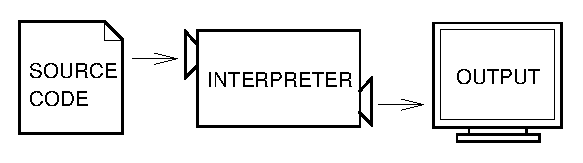
\includegraphics[height=0.77in]{figs/interpret.eps}}
\afterfig

\index{source code}
\index{object code}
\index{executable}

A compiler reads the program and translates it completely before the
program starts running.  In this context, the high-level program is
called the {\bf source code}, and the translated program is called the
{\bf object code} or the {\bf executable}.  Once a program is
compiled, you can execute it repeatedly without further translation.

\beforefig
\centerline{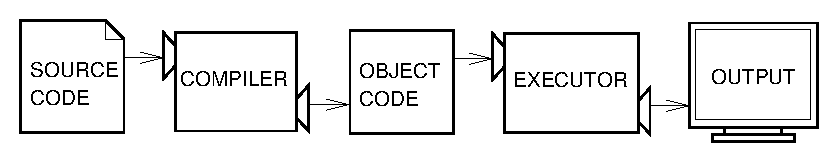
\includegraphics[height=0.77in]{figs/compile.eps}}
\afterfig

Python is considered an interpreted language because Python programs
are executed by an interpreter.  There are two ways to use the
interpreter: {\bf interactive mode} and {\bf script mode}. In
interactive mode, you type Python programs and the interpreter prints
the result:

\index{interactive mode}
\index{script mode}

\beforeverb
\begin{pyinterpreter}
>>> 1 + 1
2
\end{pyinterpreter}
\afterverb
%
The chevron, verb|>>>|, is the
{\bf prompt} the interpreter uses to indicate that it is ready.  If
you type {\tt 1 + 1}, the interpreter replies {\tt 2}.

\index{prompt}

Alternatively, you can store code in a file and use the interpreter to
execute the contents of the file, which is called a {\bf script}.  By
convention, Python scripts have names that end with {\tt .py}.
\index{script}
To execute the script, you have to tell the interpreter the name of
the file. In a Windows command shell, you would type {\tt python
	dinsdale.py}.  In other development environments, the details of
executing scripts are different.  You can find instructions for
your environment at the Python website \url{python.org}.

\index{testing!interactive mode}

Working in interactive mode is convenient for testing small pieces of
code because you can type and execute them immediately.  But for
anything more than a few lines, you should save your code
as a script so you can modify and execute it in the future.


\section{What is a program?}

A {\bf program} is a sequence of instructions that specifies how to
perform a computation.  The computation might be something
mathematical, such as solving a system of equations or finding the
roots of a polynomial, but it can also be a symbolic computation, such
as searching and replacing text in a document or (strangely enough)
compiling a program.

\index{program}

The details look different in different languages, but a few basic
instructions appear in just about every language:

\begin{description}
	
	\item[input:] Get data from the keyboard, a file, or some
	other device.
	
	\item[output:] Display data on the screen or send data to a
	file or other device.
	
	\item[math:] Perform basic mathematical operations like addition and
	multiplication.
	
	\item[conditional execution:] Check for certain conditions and
	execute the appropriate sequence of statements.
	
	\item[repetition:] Perform some action repeatedly, usually with
	some variation.
	
\end{description}

Believe it or not, that's pretty much all there is to it.  Every
program you've ever used, no matter how complicated, is made up of
instructions that look pretty much like these.  So you can think of
programming as the process of breaking a large, complex task
into smaller and smaller subtasks until the subtasks are
simple enough to be performed with one of these basic instructions.
\index{algorithm}
That may be a little vague, but we will come back to this topic
when we talk about {\bf algorithms}.

\section{What is debugging?}
\index{debugging}
\index{bug}

Programming is error-prone.  For whimsical reasons, programming errors
are called {\bf bugs} and the process of tracking them down is called
{\bf debugging}.
\index{debugging}
\index{bug}
Three kinds of errors can occur in a program: syntax errors, runtime 
errors, and semantic errors. It is useful
to distinguish between them in order to track them down more quickly.

\subsection{Syntax errors}
\index{syntax error}
\index{error!syntax}
\index{error message}

Python can only execute a program if the syntax is
correct; otherwise, the interpreter displays an error message.
{\bf Syntax} refers to the structure of a program and the rules about
that structure. \index{syntax} 
For example, parentheses have to come in matching pairs, so
{\tt (1 + 2)} is legal, but {\tt 1 + 2)} is a {\bf syntax error}.

\index{parentheses!matching}
\index{syntax}
\index{cummings, e. e.}

In English readers can tolerate most syntax errors, 
Python is not so forgiving.  If there is a single syntax error
anywhere in your program, Python will display an error message and quit,
and you will not be able to run your program. During the first few
weeks of your programming career, you will probably spend a lot of
time tracking down syntax errors.  As you gain experience, you will
make fewer errors and find them faster.

\subsection{Runtime errors}
\label{runtime}
\index{runtime error}
\index{error!runtime}
\index{exception}
\index{safe language}
\index{language!safe}

The second type of error is a runtime error, so called because the
error does not appear until after the program has started running.
These errors are also called {\bf exceptions} because they usually
indicate that something exceptional (and bad) has happened.
Runtime errors are rare in the simple programs you will see in the
first few chapters, so it might be a while before you encounter one.


\subsection{Semantic errors}
\index{semantics}
\index{semantic error}
\index{error!semantic}
\index{error message}

The third type of error is the {\bf semantic error}.  If there is a
semantic error in your program, it will run successfully in the sense
that the computer will not generate any error messages, but it will
not do the right thing.  It will do something else.  Specifically, it
will do what you told it to do.
The problem is that the program you wrote is not the program you
wanted to write.  The meaning of the program (its semantics) is wrong.
Identifying semantic errors can be tricky because it requires you to work
backward by looking at the output of the program and trying to figure
out what it is doing.

\subsection{Experimental debugging}

One of the most important skills you will acquire is debugging.
Although it can be frustrating, debugging is one of the most
intellectually rich, challenging, and interesting parts of
programming.

\index{experimental debugging}
\index{debugging!experimental}

In some ways, debugging is like detective work.  You are confronted
with clues, and you have to infer the processes and events that led
to the results you see.
Debugging is also like an experimental science.  Once you have an idea
about what is going wrong, you modify your program and try again.  If
your hypothesis was correct, then you can predict the result of the
modification, and you take a step closer to a working program.  If
your hypothesis was wrong, you have to come up with a new one.  As
Sherlock Holmes pointed out~\parencite{doyle2010sign}, ``When you have eliminated the
impossible, whatever remains, however improbable, must be the truth.''


For some people, programming and debugging are the same thing.  That
is, programming is the process of gradually debugging a program until
it does what you want.  The idea is that you should start with a
program that does {\em something} and make small modifications,
debugging them as you go, so that you always have a working program.

For example, Linux is an operating system that contains thousands of
lines of code, but it started out as a simple program Linus Torvalds
used to explore the Intel 80386 chip.  According to Larry Greenfield,
``One of Linus's earlier projects was a program that would switch
between printing AAAA and BBBB.  This later evolved to Linux.''
({\em The Linux Users' Guide} Beta Version 1).

\index{Linux}

Later chapters will make more suggestions about debugging and other
programming practices.

\section{Formal and natural languages}
\index{formal language}
\index{natural language}
\index{language!formal}
\index{language!natural}

\begin{definition}[Natural languages] are the languages people speak,
such as English, Spanish, and French.  They were not designed
by people (although people try to impose some order on them);
they evolved naturally.
\end{definition}

\begin{definition}[Formal languages] are languages that are designed by people for
specific applications.  For example, the notation that mathematicians
use is a formal language that is particularly good at denoting
relationships among numbers and symbols.  Chemists use a formal
language to represent the chemical structure of molecules.  And
most importantly:
\end{definition}

\begin{quote}
	{\bf Programming languages are formal languages that have been
		designed to express computations.}
\end{quote}

Formal languages tend to have strict rules about syntax.  For example,
$3 + 3 = 6$ is a syntactically correct mathematical statement, but 
$3 + = 6 \mbox{\pounds} 3$ is not. 
Syntax rules come in two flavors, pertaining to {\bf tokens} and
structure.  Tokens are the basic elements of the language, such as
words, numbers, operators.  One of the problems with $3 +
= 3 \mbox{\pounds} 6$ is that $\pounds$ is not a legal token in mathematics.

\index{token}
\index{structure}

The second type of syntax error pertains to the structure of a
statement; that is, the way the tokens are arranged.  The statement $3
+ = 6 - 3$ is illegal because even though $+$ and $=$ are
legal tokens, you can't have one right after the other.

When you read a sentence in English or a statement in a formal
language, you have to figure out what the structure of the sentence is
(although in a natural language you do this subconsciously).  This
process is called {\bf parsing}.

\index{parse}

For example, when you hear the sentence, ``The penny dropped,'' you
understand that ``the penny'' is the subject and ``dropped'' is the
predicate.  Once you have parsed a sentence, you can figure out what it
means, or the semantics of the sentence.  Assuming that you know
what a penny is and what it means to drop, you will understand the
general implication of this sentence.

Although formal and natural languages have many features in
common---tokens, structure, syntax, and semantics---there are some
important differences:

\index{ambiguity}
\index{redundancy}
\index{literalness}

\begin{description}
	
	\item[ambiguity:] Natural languages are full of ambiguity, which
	people deal with by using contextual clues and other information.
	Formal languages are designed to be nearly or completely unambiguous,
	which means that any statement has exactly one meaning,
	regardless of context.
	
	\item[redundancy:] In order to make up for ambiguity and reduce
	misunderstandings, natural languages employ lots of
	redundancy.  As a result, they are often verbose.  Formal languages
	are less redundant and more concise.
	
	\item[literalness:] Natural languages are full of idiom and metaphor.
	If I say, ``The penny dropped,'' there is probably no penny and
	nothing dropping\footnote{This idiom means that someone realized something
		after a period of confusion.}.  Formal languages
	mean exactly what they say.
	
\end{description}

Here are some suggestions for reading programs (and other formal
languages).  First, remember that formal languages are much more dense
than natural languages, so it takes longer to read them.  Also, the
structure is very important, so it is usually not a good idea to read
from top to bottom, left to right.  Instead, learn to parse the
program in your head, identifying the tokens and interpreting the
structure.  Finally, the details matter.  Small errors in
spelling and punctuation, which you can get away
with in natural languages, can make a big difference in a formal
language.

\section{The first program}
\label{hello}

\index{Hello, World}

Traditionally, the first program you write in a new language
is called ``Hello, World!'' because all it does is display the
words, ``Hello, World!''  In Python 3, it looks like this:

\beforeverb
\begin{pyinterpreter}
>>> print('Hello, World!')
Hello, World!
\end{pyinterpreter}
\afterverb
%

The quotation marks in the program mark the beginning and end
of the text to be displayed; they don't appear in the result.

\index{quotation mark}
\index{print statement}
\index{statement!print}

Some people judge the quality of a programming language by the
simplicity of the ``Hello, World!'' program.  By this standard, Python
does about as well as possible.


\section{Debugging}
\index{debugging}

It is a good idea to read this book in front of a computer so you can
try out the examples as you go.  You can run most of the examples in
interactive mode, but if you put the code into a script, it is easier
to try out variations.
Whenever you are experimenting with a new feature, you should try
to make mistakes.  For example, in the ``Hello, world!'' program,
what happens if you leave out one of the quotation marks?  What
if you leave out both?  What if you spell {\tt print} wrong?

\index{error message}

\begin{remark}
This kind of experiment helps you remember what you read; it also helps
with debugging, because you get to know what the error messages mean.
It is better to make mistakes now and on purpose than later
and accidentally.
\end{remark}

Programming, and especially debugging, sometimes brings out strong
emotions.  If you are struggling with a difficult bug, you might 
feel angry, despondent or embarrassed.
There is evidence that people naturally respond to computers as if
they were people\footnote{See Reeves and Nass, {\it The Media
		Equation: How People Treat Computers, Television, and New Media
		Like Real People and Places}.}.  
When they work well, we think
of them as teammates, and when they are obstinate or rude, we
respond to them the same way we respond to rude,
obstinate people.
Preparing for these reactions might help you deal with them.
One approach is to think of the computer as an employee with
certain strengths, like speed and precision, and
particular weaknesses, like lack of empathy and inability
to grasp the big picture.
Your job is to be a good manager: find ways to take advantage
of the strengths and mitigate the weaknesses.  And find ways
to use your emotions to engage with the problem,
without letting your reactions interfere with your ability
to work effectively.

Learning to debug can be frustrating, but it is a valuable skill
that is useful for many activities beyond programming.  At the
end of each chapter there is a debugging section, like this one,
with my thoughts about debugging.  I hope they help!


\section{Glossary}
	
\begin{vocabulary}[problem solving:]  
The process of formulating a problem, finding a solution, and expressing the solution.
	\index{problem solving}
\end{vocabulary}
	
\begin{vocabulary}[high-level language:]  A programming language like Python that
	is designed to be easy for humans to read and write.
	\index{high-level language}
\end{vocabulary}
	
\begin{vocabulary}[low-level language:]  A programming language that is designed
	to be easy for a computer to execute; also called ``machine language'' or
	``assembly language.''
	\index{low-level language}
\end{vocabulary}
	
\begin{vocabulary}[portability:]  A property of a program that can run on more
	than one kind of computer.
	\index{portability}
\end{vocabulary}
	
\begin{vocabulary}[interpret:]  To execute a program in a high-level language
	by translating it one line at a time.
	\index{interpret}
\end{vocabulary}
	
\begin{vocabulary}[compile:]  To translate a program written in a high-level language
	into a low-level language all at once, in preparation for later
	execution.
	\index{compile}
\end{vocabulary}
	
\begin{vocabulary}[source code:]  A program in a high-level language before
	being compiled.
	\index{source code}
\end{vocabulary}
	
\begin{vocabulary}[object code:]  The output of the compiler after it translates
	the program.
	\index{object code}
\end{vocabulary}
	
\begin{vocabulary}[executable:]  Another name for object code that is ready
	to be executed.
	\index{executable}
\end{vocabulary}
	
\begin{vocabulary}[prompt:] Characters displayed by the interpreter to indicate
	that it is ready to take input from the user.
	\index{prompt}
\end{vocabulary}
	
\begin{vocabulary}[script:] A program stored in a file (usually one that will be
	interpreted).
	\index{script}
\end{vocabulary}
	
\begin{vocabulary}[interactive mode:] A way of using the Python interpreter by
	typing commands and expressions at the prompt.
	\index{interactive mode}
\end{vocabulary}
	
\begin{vocabulary}[script mode:] A way of using the Python interpreter to read
	and execute statements in a script.
	\index{script mode}
\end{vocabulary}
	
\begin{vocabulary}[program:] A set of instructions that specifies a computation.
	\index{program}
\end{vocabulary}
	
\begin{vocabulary}[algorithm:]  A general process for solving a category of
	problems.
	\index{algorithm}
\end{vocabulary}
	
\begin{vocabulary}[bug:]  An error in a program.
	\index{bug}
\end{vocabulary}
	
\begin{vocabulary}[debugging:]  The process of finding and removing any of the
	three kinds of programming errors.
\end{vocabulary}
	
\begin{vocabulary}[syntax:]  The structure of a program.
	\index{syntax}
\end{vocabulary}
	
\begin{vocabulary}[syntax error:]  An error in a program that makes it impossible
	to parse (and therefore impossible to interpret).
	\index{syntax error}
\end{vocabulary}
	
\begin{vocabulary}[exception:]  An error that is detected while the program is running.
	\index{exception}
\end{vocabulary}
	
\begin{vocabulary}[semantics:]  The meaning of a program.
	\index{semantics}
\end{vocabulary}
	
\begin{vocabulary}[semantic error:]   An error in a program that makes it do something
	other than what the programmer intended.
	\index{semantic error}
\end{vocabulary}
	
\begin{vocabulary}[natural language:]  Any one of the languages that people speak that
	evolved naturally.
	\index{natural language}
\end{vocabulary}
	
\begin{vocabulary}[formal language:]  Any one of the languages that people have designed
	for specific purposes, such as representing mathematical ideas or
	computer programs; all programming languages are formal languages.
	\index{formal language}
\end{vocabulary}
	
\begin{vocabulary}[token:]  One of the basic elements of the syntactic structure of
	a program, analogous to a word in a natural language.
	\index{token}
\end{vocabulary}
	
\begin{vocabulary}[parse:]  To examine a program and analyze the syntactic structure.
	\index{parse}
\end{vocabulary}
	
\begin{vocabulary}[print statement:]  An instruction that causes the Python
	interpreter to display a value on the screen.
	\index{print statement}
	\index{statement!print}
\end{vocabulary}


\section{Exercises}

\begin{exercise}
	Use a web browser to go to the Python website \url{python.org}.
	This page contains information about Python and links
	to Python-related pages, and it gives you the ability to search
	the Python documentation.
	
	For example, if you enter {\tt print} in the search window, the
	first link that appears is the documentation of the {\tt print}
	statement.  At this point, not all of it will make sense to you,
	but it is good to know where it is.
	
	\index{documentation}
	\index{python.org}
\end{exercise}

\begin{exercise}
	Start the Python interpreter and type {\tt help()} to start the online
	help utility.  Or you can type \verb"help('print')" to get information
	about the {\tt print} statement.
	
	If this example doesn't work, you
	may need to install additional Python documentation or set an
	environment variable; the details depend on your operating system and
	version of Python.
	%
	\index{help utility}
\end{exercise}

\begin{exercise}
	Start the Python interpreter and use it as a calculator.
	Python's syntax for math operations is almost the same as
	standard mathematical notation.  For example, the symbols
	{\tt +}, {\tt -} and {\tt /} denote addition, subtraction
	and division, as you would expect.  The symbol for
	multiplication is {\tt *}.
	
	If you run a 10 kilometer race in 43 minutes 30 seconds, what is your
	average time per mile?  What is your average speed in miles per hour?
	(Hint: there are 1.61 kilometers in a mile).
	%
	\index{calculator}
	\index{running pace}
	
\end{exercise}

%
%\chapterimage{chapter_head_2.pdf} % Chapter heading image
\chapter{Variables, expressions and statements}

\section{Values and types}
\index{value}
\index{type}
\index{string}

A {\bf value} is one of the basic things a program works with,
like a letter or a
number.  The values we have seen so far
are {\tt 1}, {\tt 2}, and
\verb"'Hello, World!'".

These values belong to different {\bf types} also known as {\bf classes} in Python 3. For example,
{\tt 2} is an integer, and \verb"'Hello, World!'" is a {\bf string},
so-called because it contains a ``string'' of letters.
You (and the interpreter) can identify
strings because they are enclosed in quotation marks.

\index{quotation mark}

The print statement also works for integers.

\beforeverb
\begin{pyinterpreter}
>>> print(4)
4
\end{pyinterpreter}
\afterverb
%
If you are not sure what type a value has, the interpreter can tell you.

\beforeverb
\begin{pyinterpreter}
>>> type('Hello, World!')
<class 'str'>
>>> type(17)
<class 'int'>
\end{pyinterpreter}
\afterverb
%
Not surprisingly, strings belong to the type (class) {\tt str} and
integers belong to the type (class) {\tt int}.  Less obviously, numbers
with a decimal point belong to a type called {\tt float},
because these numbers are represented in a
format called {\bf floating-point}.

\index{type}
\index{string type}
\index{type!str}
\index{int type}
\index{type!int}
\index{float type}
\index{type!float}

\beforeverb
\begin{pyinterpreter}
>>> type(3.2)
<class 'float'>
\end{pyinterpreter}
\afterverb
%
What about values like \verb"'17'" and \verb"'3.2'"?
They look like numbers, but they are in quotation marks like
strings.
%
\index{quotation mark}
%
\beforeverb
\begin{pyinterpreter}
>>> type('17')
<class 'str'>
>>> type('3.2')
<class 'str'>
\end{pyinterpreter}
\afterverb
%
They are strings.

When you type a large integer, you might be tempted to use commas
between groups of three digits, as in {\tt 1,000,000}.  This is not a
legal integer in Python, but it is legal:

\beforeverb
\begin{pyinterpreter}
>>> print(1,000,000)
1 0 0
\end{pyinterpreter}
\afterverb
%
Well, that's not what we expected at all!  Python interprets {\tt
  1,000,000} as a comma-separated sequence of integers, which it
prints with spaces between.
%
\index{semantic error}
\index{error!semantic}
\index{error message}
%
This is the first example we have seen of a semantic error: the code
runs without producing an error message, but it doesn't do the
``right'' thing.


\section{Variables}
\index{variable}
\index{assignment statement}
\index{statement!assignment}

One of the most powerful features of a programming language is the
ability to manipulate {\bf variables}.  A variable is a name that
refers to a value.

An {\bf assignment statement} creates new variables and gives
them values:

\beforeverb
\begin{pyinterpreter}
>>> message = 'And now for something completely different'
>>> n = 17
>>> pi = 3.1415926535897931
\end{pyinterpreter}
\afterverb
%
This example makes three assignments.  The first assigns a string
to a new variable named {\tt message};
the second gives the integer {\tt 17} to {\tt n}; the third
assigns the (approximate) value of $\pi$ to {\tt pi}.

\index{state diagram}
\index{diagram!state}

A common way to represent variables on paper is to write the name with
an arrow pointing to the variable's value.  This kind of figure is
called a {\bf state diagram} because it shows what state each of the
variables is in (think of it as the variable's state of mind).
This diagram shows the result of the previous example:

\beforefig
\centerline{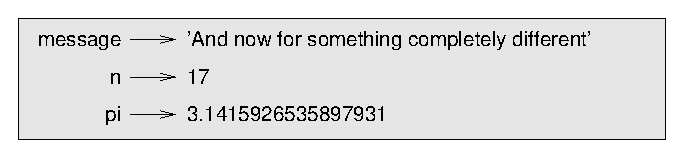
\includegraphics{figs/state2.eps}}
\afterfig

To display the value of a variable, you can use a print statement:

\beforeverb
\begin{pyinterpreter}
>>> print(n)
17
>>> print(pi)
3.14159265359
\end{pyinterpreter}
\afterverb
%
The type of a variable is the type of the value it refers to.

\beforeverb
\begin{pyinterpreter}
>>> type(message)
<class 'str'>
>>> type(n)
<class 'int'>
>>> type(pi)
<class 'float'>
\end{pyinterpreter}
\afterverb
%
\begin{remark}
If you type an integer with a leading zero, you might get
a confusing error:

\beforeverb
\begin{pyinterpreter}
>>> zipcode = 02492
                  ^
SyntaxError: invalid token
\end{pyinterpreter}
\afterverb
\end{remark}




\section{Variable names and keywords}
\index{keyword}

Programmers generally choose names for their variables that
are meaningful---they document what the variable is used for.
Variable names can be arbitrarily long.  They can contain
both letters and numbers, but they have to begin with a letter.
It is legal to use uppercase letters, but it is a good idea
to begin variable names with a lowercase letter (you'll
see why later).
The underscore character (\verb"_") can appear in a name.
It is often used in names with multiple words, such as
\verb"my_name" or \verb"airspeed_of_unladen_swallow".

\index{underscore character}

If you give a variable an illegal name, you get a syntax error:

\beforeverb
\begin{pyinterpreter}
>>> 76trombones = 'big parade'
SyntaxError: invalid syntax
>>> more@ = 1000000
SyntaxError: invalid syntax
>>> class = 'Advanced Theoretical Zymurgy'
SyntaxError: invalid syntax
\end{pyinterpreter}
\afterverb
%
{\tt 76trombones} is illegal because it does not begin with a letter.
{\tt more@} is illegal because it contains an illegal character, {\tt
@}.  But what's wrong with {\tt class}?
It turns out that {\tt class} is one of Python's {\bf keywords}.  The
interpreter uses keywords to recognize the structure of the program,
and they cannot be used as variable names.
Python 3 has 33 keywords has shown in Table~\ref{tab:python_keywords}.
\index{keyword}

\begin{table}[htb]
\begin{center}
\begin{tabular}{p{2cm} p{2cm} p{2cm} p{2cm} p{2cm}}
False & class & finally & is & return\\
None & continue & for & lambda & try\\
True & def & from & nonlocal & while\\
and & del & global & not & with\\
as & elif & if & or & yield\\
assert & else & import & pass & \\
break & except & in & raise & \\
\end{tabular}
\caption{Keywords in Python 3 programming language.}
\label{tab:python_keywords} 
\end{center}
\end{table}
%
You might want to keep this list handy.  If the interpreter complains
about one of your variable names and you don't know why, see if it
is on this list.


\section{Statements}

A statement is a unit of code that the Python interpreter can
execute.  We have seen two kinds of statements: print
and assignment.
%
\index{statement}
\index{interactive mode}
\index{script mode}
%
When you type a statement in interactive mode, the interpreter
executes it and displays the result, if there is one.
%
A script usually contains a sequence of statements.  If there
is more than one statement, the results appear one at a time
as the statements execute.

For example, the script

\beforeverb
\begin{pycode}
print(1)
x = 2
print(x)
\end{pycode}
\afterverb
%
produces the output

\beforeverb
\begin{pyoutput}
1
2
\end{pyoutput}
\afterverb
%
The assignment statement produces no output.


\section{Operators and operands}
\index{operator, arithmetic}
\index{arithmetic operator}
\index{operand}
\index{expression}

{\bf Operators} are special symbols that represent computations like
addition and multiplication.  The values the operator is applied to
are called {\bf operands}.
The operators {\tt +}, {\tt -}, {\tt *}, {\tt /} and {\tt **}
perform addition, subtraction, multiplication, division and
exponentiation, as in the following examples:

\beforeverb
\begin{pyinterpreter}
20+32   hour-1   hour*60+minute   minute/60   5**2   (5+9)*(15-7)
\end{pyinterpreter}
\afterverb
%

%When a variable name appears in the place of an operand, it
%is replaced with its value before the operation is
%performed.

Python 3, as well as other languages have an {\bf integer division} {\tt //}. The integer division operate a {\bf floor division}, that is the operator returns the whole part of the division. The result of the integer division  is an integer. If both operands are integer the value returned is a integer. Otherwise, if at least one of the operand is a float, the value returned is a float.

\beforeverb
\begin{pyinterpreter}
>>> minute = 59
>>> minute // 60
0
>>> minute = 61
>>> minute // 60
1
>>> minute // 60.0
1.0
>>> minute / 60.0
1.0166666666666666
\end{pyinterpreter}
\afterverb
%
\index{Python 3.0}
\index{floor division}
\index{floating-point division}
\index{division!floor}
\index{division!floating-point}
\index{division!integer division}

\section{Expressions}

An {\bf expression} is a combination of values, variables, and operators.
A value all by itself is considered an expression, and so is
a variable, so the following are all legal expressions
(assuming that the variable {\tt x} has been assigned a value):

\index{expression}
\index{evaluate}

\beforeverb
\begin{pycode}
17
x
x + 17
\end{pycode}
\afterverb
%
If you type an expression in interactive mode, the interpreter
{\bf evaluates} it and displays the result:

\beforeverb
\begin{pyinterpreter}
>>> 1 + 1
2
\end{pyinterpreter}
\afterverb
%
But in a script, an expression all by itself doesn't
do anything!  This is a common
source of confusion for beginners.

\begin{exercise}
Type the following statements in the Python interpreter to see
what they do:

\beforeverb
\begin{pyexo}
5
x = 5
x + 1
\end{pyexo}
\afterverb
%
Now put the same statements into a script and run it.  What
is the output?  Modify the script by transforming each
expression into a print statement and then run it again.
\end{exercise}


\section{Order of operations}
\index{order of operations}
\index{rules of precedence}
\index{PEMDAS}

When more than one operator appears in an expression, the order of
evaluation depends on the {\bf rules of precedence}.  For
mathematical operators, Python follows mathematical convention.
The acronym {\bf PEMDAS} is a useful way to
remember the rules:

\index{parentheses!overriding precedence}

\begin{itemize}

\item {\bf P}arentheses have the highest precedence and can be used 
to force an expression to evaluate in the order you want. Since
expressions in parentheses are evaluated first, {\tt 2 * (3-1)} is 4,
and {\tt (1+1)**(5-2)} is 8. You can also use parentheses to make an
expression easier to read, as in {\tt (minute * 100) / 60}, even
if it doesn't change the result.

\item {\bf E}xponentiation has the next highest precedence, so
{\tt 2**1+1} is 3, not 4, and {\tt 3*1**3} is 3, not 27.

\item {\bf M}ultiplication and {\bf D}ivision have the same precedence,
which is higher than {\bf A}ddition and {\bf S}ubtraction, which also
have the same precedence.  So {\tt 2*3-1} is 5, not 4, and
{\tt 6+4/2} is 8, not 5.

\item Operators with the same precedence are evaluated from left to 
right.  So in the expression {\tt degrees/2*pi}, the division
happens first and the result is multiplied by {\tt pi}, therefore the expression is equal to $\frac{\pi}{2}degrees$. To divide by $2 \pi$, you can use parentheses (e.g. {\tt degrees/(2*pi)}) or write {\tt degrees/2/pi}.

\end{itemize}

\begin{table}[htb]
\begin{center}
\begin{tabular}{|p{3cm}|p{7cm}|}
\hline
Operator & Description\\\hline
** & Exponentiation (raise to the power)\\
+, - & Unary plus and minus (method names for the last two are +@ and -@)\\
*, /, \%, //  & Multiply, divide, modulo and floor division\\
+, - & Addition and subtraction\\
%>>, << & Right and left bitwise shift\\
%\& & Bitwise 'AND'\\
%$\hat$, \| & Bitwise exclusive `OR' and regular `OR'\\
<=, <, >, >= & Comparison operators\\
<>, ==, != & Equality operators\\
\verb|is|, \verb|is not| & Identity operators\\
\verb|in|, \verb|not in| & Membership operators\\
\verb|not| & Logical operators\\
\verb|and| & Logical operators\\
\verb|or|  & Logical operators\\
= ,\%=, /=, //=, -=, +=, *=, **= & Assignment operators\\\hline
\end{tabular}
\caption{Operators precedence in Python from highest precedence (top) to lowest (bottom).}
\label{tab:operator_precedence}
\end{center}
\end{table}

\section{String operations}
\index{string!operation}
\index{operator!string}

In general, you cannot perform mathematical operations on strings, even
if the strings look like numbers, so the following are illegal:

\beforeverb
\begin{pyinterpreter}
'2'-'1'    'eggs'/'easy'    'third'*'a charm'
\end{pyinterpreter}
\afterverb
%
The {\tt +} operator works with strings, but it
might not do what you expect: it performs
{\bf concatenation}, which means joining the strings by
linking them end-to-end.  For example:

\index{concatenation}

\beforeverb
\begin{pycode}
first = 'throat'
second = 'warbler'
print(first + second)
\end{pycode}
\afterverb
%
The output of this program is {\tt throatwarbler}.

The {\tt *} operator also works on strings; it performs repetition.
For example, \verb"'Spam'*3" is \verb"'SpamSpamSpam'".  If one of the operands
is a string, the other has to be an integer.
This use of {\tt +} and {\tt *} makes sense by
analogy with addition and multiplication.  Just as {\tt 4*3} is
equivalent to {\tt 4+4+4}, we expect \verb"'Spam'*3" to be the same as
\verb"'Spam'+'Spam'+'Spam'", and it is.  

On the other hand, there is a significant way in which string concatenation 
is different from integer addition. Concatenation is not commutative, which
 means that \verb"'spam'+'sandwich'" is not the same as \verb"'sandwich'+'spam'",
 whereas {\tt 3+4} is the same as {\tt 4+3}.

\index{commutativity}


\section{Comments}
\index{comment}

As programs get bigger and more complicated, they get more difficult
to read.  Formal languages are dense, and it is often difficult to
look at a piece of code and figure out what it is doing, or why.
For this reason, it is a good idea to add notes to your programs to explain
in natural language what the program is doing.  These notes are called
{\bf comments}, and they start with the \verb"#" symbol:

\beforeverb
\begin{pycode}
# compute the percentage of the hour that has elapsed
percentage = (minute * 100) / 60
\end{pycode}
\afterverb
%
In this case, the comment appears on a line by itself.  You can also put
comments at the end of a line:

\beforeverb
\begin{pycode}
percentage = (minute * 100) / 60     # percentage of an hour
\end{pycode}
\afterverb
%
Everything from the {\tt \#} to the end of the line is ignored---it
has no effect on the program.

Comments are most useful when they document non-obvious features of
the code.  It is reasonable to assume that the reader can figure out
{\em what} the code does; it is much more useful to explain {\em why}.

This comment is redundant with the code and useless:

\beforeverb
\begin{pycode}
v = 5     # assign 5 to v
\end{pycode}
\afterverb
%
Such comments are not helping the readability of the code, on the contrary. It is likely that a developer reading your code will stop paying attention to your comments as most of them will be useless. As a consequence, important aspects of your code that have been described in comments will be ignored. On the other hand, the following comment contains useful information that is not in the code:

\beforeverb
\begin{pycode}
v = 5     # velocity in meters/second. 
\end{pycode}
\afterverb
%
Good variable names can reduce the need for comments, but
long names can make complex expressions hard to read, so there is
a tradeoff.

\section{Debugging}
\index{debugging}

At this point the syntax error you are most likely to make is
an illegal variable name, like {\tt class} and {\tt yield}, which
are keywords, or \verb"odd~job" and \verb"GBP£", which contain
illegal characters.

\index{syntax error}
\index{error!syntax}

If you put a space in a variable name, Python thinks it is two
operands without an operator:

\beforeverb
\begin{pyinterpreter}
>>> bad name = 5
SyntaxError: invalid syntax
\end{pyinterpreter}
\afterverb
%
For syntax errors, the error messages don't help much.
The most common messages are {\tt SyntaxError: invalid syntax} and
{\tt SyntaxError: invalid token}, neither of which is very informative.

\index{error message}
\index{use before def}
\index{exception}
\index{runtime error}
\index{error!runtime}

The runtime error you are most likely to make is a \verb|NameError| that is, trying to use a variable before you have assigned a value.  This can happen if you spell a variable name wrong:

\beforeverb
\begin{pyinterpreter}
>>> principal = 327.68
>>> interest = principle * rate
Traceback (most recent call last):
  File "<pyshell#36>", line 1, in <module>
    interest = principle * rate
NameError: name 'principle' is not defined
\end{pyinterpreter}
\afterverb
%
Variables names are case sensitive, so {\tt Principal} is not the
same as {\tt principal}.

\index{case-sensitivity, variable names}
\index{semantic error}
\index{error!semantic}

At this point the most likely cause of a semantic error is
the order of operations.  For example, to evaluate $\frac{1}{2 \pi}$,
you might be tempted to write

\beforeverb
\begin{pyinterpreter}
>>> 1.0 / 2.0 * pi
\end{pyinterpreter}
\afterverb
%
But the division happens first, so you would get $\pi / 2$, which
is not the same thing!  There is no way for Python
to know what you meant to write, so in this case you don't
get an error message; you just get the wrong answer.

\index{order of operations}


\section{Glossary}

\begin{vocabulary}[value:]  One of the basic units of data, like a number or string, 
that a program manipulates.
\index{value}
\end{vocabulary}
	
\begin{vocabulary}[type:] A category of values.  The types we have seen so far
are integers (type {\tt int}), floating-point numbers (type {\tt
float}), and strings (type {\tt str}).
\index{type}
\end{vocabulary}
	
\begin{vocabulary}[integer:] A type that represents whole numbers.
\index{integer}
\end{vocabulary}
	
\begin{vocabulary}[floating-point:] A type that represents numbers with fractional
parts.
\index{floating-point}
\end{vocabulary}
	
\begin{vocabulary}[string:] A type that represents sequences of characters.
\index{string}
\end{vocabulary}
	
\begin{vocabulary}[variable:]  A name that refers to a value.
\index{variable}
\end{vocabulary}
	
\begin{vocabulary}[statement:]  A section of code that represents a command or action.  So
far, the statements we have seen are assignments and print statements.
\index{statement}
\end{vocabulary}
	
\begin{vocabulary}[assignment:]  A statement that assigns a value to a variable.
\index{assignment}
\end{vocabulary}
	
\begin{vocabulary}[state diagram:]  A graphical representation of a set of variables and the
values they refer to.
\index{state diagram}
\end{vocabulary}
	
\begin{vocabulary}[keyword:]  A reserved word that is used by the compiler to parse a
program; you cannot use keywords like {\tt if}, {\tt  def}, and {\tt while} as
variable names.
\index{keyword}
\end{vocabulary}
	
\begin{vocabulary}[operator:]  A special symbol that represents a simple computation like
addition, multiplication, or string concatenation.
\index{operator}
\end{vocabulary}
	
\begin{vocabulary}[operand:]  One of the values on which an operator operates.
\index{operand}

\item[floor division:] The operation that divides two numbers and chops off
the fraction part.
\index{floor division}
\end{vocabulary}
	
\begin{vocabulary}[expression:]  A combination of variables, operators, and values that
represents a single result value.
\index{expression}
\end{vocabulary}
	
\begin{vocabulary}[evaluate:]  To simplify an expression by performing the operations
in order to yield a single value.
\end{vocabulary}
	
\begin{vocabulary}[rules of precedence:]  The set of rules governing the order in which
expressions involving multiple operators and operands are evaluated.
\index{rules of precedence}
\index{precedence}
\end{vocabulary}
	
\begin{vocabulary}[concatenate:]  To join two operands end-to-end.
\index{concatenation}
\end{vocabulary}
	
\begin{vocabulary}[comment:]  Information in a program that is meant for other
programmers (or anyone reading the source code) and has no effect on the
execution of the program.
\index{comment}
\end{vocabulary}
	

\section{Exercises}

\begin{exercise}
Assume that we execute the following assignment statements:

\begin{pyexo}
width = 17
height = 12.0
delimiter = '.'
\end{pyexo}

For each of the following expressions, write the value of the
expression and the type (of the value of the expression).

\begin{enumerate}

\item {\tt width/2}

\item {\tt width/2.0}

\item {\tt height/3}

\item {\tt 1 + 2 * 5}

\item {\tt delimiter * 5}

\end{enumerate}

Use the Python interpreter to check your answers.
\end{exercise}

\begin{exercise}
Practice using the Python interpreter as a calculator: 
\index{calculator}

\begin{enumerate}

\item The volume of a sphere with radius $r$ is $\frac{4}{3} \pi r^3$.
  What is the volume of a sphere with radius 5?  Hint: 392.6 is wrong!

\item Suppose the cover price of a book is \$24.95, but bookstores get a
  40\% discount.  Shipping costs \$3 for the first copy and 75 cents
  for each additional copy.  What is the total wholesale cost for
  60 copies?

\item If I leave my house at 6:52 am and run 1 mile at an easy pace
  (8:15 per mile), then 3 miles at tempo (7:12 per mile) and 1 mile at
  easy pace again, what time do I get home for breakfast?

\index{running pace}

\end{enumerate}
\end{exercise}

%
%\chapterimage{chapter_head_1.pdf} % Chapter heading image
\chapter{Functions}
\label{funcchap}

\section{Function calls}
\label{functionchap}
\index{function call}

In the context of programming, a {\bf function} is a named sequence of
statements that performs a computation.  When you define a function,
you specify the name and the sequence of statements.  Later, you can
``call'' the function by name.  
We have already seen one example of a {\bf function call}:

\beforeverb
\begin{pyinterpreter}
>>> type(32)
<type 'int'>
\end{pyinterpreter}
\afterverb
%
The name of the function is {\tt type}.  The expression in parentheses
is called the {\bf argument} of the function.  The result, for this
function, is the type of the argument.

\index{parentheses!argument in}

It is common to say that a function ``takes'' an argument and ``returns''
a result.  The result is called the {\bf return value}.

\index{argument}
\index{return value}


\section{Type conversion functions}
\index{conversion!type}
\index{type conversion}

% from Elkner:
% comment on whether these things are _really_ functions?
% use max as an example of a built-in?

% my reply:
% they are on the list of ``built-in functions'' so I am
% willing to call them functions.

Python provides built-in functions that convert values
from one type to another.  The {\tt int} function takes any value and
converts it to an integer, if it can, or complains otherwise:

\index{int function}
\index{function!int}

\beforeverb
\begin{pyinterpreter}
>>> int('32')
32
>>> int('Hello')
Traceback (most recent call last):
  File "<pyshell#40>", line 1, in <module>
    int('hello')
ValueError: invalid literal for int() with base 10: 'Hello'
\end{pyinterpreter}
\afterverb
%
{\tt int} can convert floating-point values to integers, but it
doesn't round off; it chops off the fraction part:

\beforeverb
\begin{pyinterpreter}
>>> int(3.99999)
3
>>> int(-2.3)
-2
\end{pyinterpreter}
\afterverb
%
{\tt float} converts integers and strings to floating-point
numbers:

\index{float function}
\index{function!float}

\beforeverb
\begin{pyinterpreter}
>>> float(32)
32.0
>>> float('3.14159')
3.14159
\end{pyinterpreter}
\afterverb
%
Finally, {\tt str} converts its argument to a string:

\index{str function}
\index{function!str}

\beforeverb
\begin{pyinterpreter}
>>> str(32)
'32'
>>> str(3.14159)
'3.14159'
\end{pyinterpreter}
\afterverb
%



\section{Math functions}
\index{math function}
\index{function, math}

Python has a math module that provides most of the familiar
mathematical functions.  A {\bf module} is a file that contains a
collection of related functions.

\index{module}
\index{module object}

Before we can use the module, we have to import it:

\beforeverb
\begin{pyinterpreter}
>>> import math
\end{pyinterpreter}
\afterverb
%
This statement creates a {\bf module object} named math.
%
The module object contains the functions and variables defined in the
module.  To access one of the functions, you have to specify the name
of the module and the name of the function, separated by a dot (also
known as a period).  This format is called {\bf dot notation}.

\index{dot notation}

\beforeverb
\begin{pyinterpreter}
>>> ratio = signal_power / noise_power
>>> decibels = 10 * math.log10(ratio)

>>> radians = 0.7
>>> height = math.sin(radians)
\end{pyinterpreter}
\afterverb
%
The first example computes the logarithm base 10 of the
signal-to-noise ratio.  The math module also provides a
function called {\tt log} that computes logarithms base {\tt e}.

\index{log function}
\index{function!log}
\index{sine function}
\index{radian}
\index{trigonometric function}
\index{function, trigonometric}

The second example finds the sine of {\tt radians}.  The name of the
variable is a hint that {\tt sin} and the other trigonometric
functions ({\tt cos}, {\tt tan}, etc.)  take arguments in radians. To
convert from degrees to radians, divide by 360 and multiply by $2
\pi$:

\beforeverb
\begin{pyinterpreter}
>>> degrees = 45
>>> radians = degrees / 360.0 * 2 * math.pi
>>> math.sin(radians)
0.707106781187
\end{pyinterpreter}
\afterverb
%
The expression {\tt math.pi} gets the variable {\tt pi} from the math
module.  The value of this variable is an approximation
of $\pi$, accurate to about 15 digits.

\index{pi}

%COMMENT: the following section has been removed as it does not help comprehension 
%If you know
%your trigonometry, you can check the previous result by comparing it to
%the square root of two divided by two:
%
%\index{sqrt function}
%\index{function!sqrt}
%
%\beforeverb
%\begin{pyinterpreter}
%>>> math.sqrt(2) / 2.0
%0.707106781187
%\end{pyinterpreter}
%\afterverb
%

\section{Composition}
\index{composition}

So far, we have looked at the elements of a program---variables,
expressions, and statements---in isolation, without talking about how to
combine them.

One of the most useful features of programming languages is their
ability to take small building blocks and {\bf compose} them.  For
example, the argument of a function can be any kind of expression,
including arithmetic operators:

\beforeverb
\begin{pyinterpreter}
x = math.sin(degrees / 360.0 * 2 * math.pi)
\end{pyinterpreter}
\afterverb
%
And even function calls:

\beforeverb
\begin{pyinterpreter}
x = math.exp(math.log(x+1))
\end{pyinterpreter}
\afterverb
%
Almost anywhere you can put a value, you can put an arbitrary
expression, with one exception: the left side of an assignment
statement has to be a variable name.  Any other expression on the left
side is a syntax error\footnote{We will see exceptions to this rule
later.}.

\beforeverb
\begin{pyinterpreter}
>>> hours = 2              # correct
>>> minutes = hours * 60   # correct
>>> hours * 2 = minutes    # wrong
SyntaxError: can't assign to operator
\end{pyinterpreter}
\afterverb
%
\index{SyntaxError}
\index{exception!SyntaxError}


\section{Adding new functions}

So far, we have only been using the functions that come with Python,
but it is also possible to add new functions.
A {\bf function definition} specifies the name of a new function and
the sequence of statements that execute when the function is called.

\index{function}
\index{function definition}
\index{definition!function}

Here is an example:

\beforeverb
\begin{pycode}
def print_lyrics():
    print("I'm a lumberjack, and I'm okay.")
    print("I sleep all night and I work all day.")
\end{pycode}
\afterverb
%
{\tt def} is a keyword that indicates that this is a function
definition.  The name of the function is \verb"print_lyrics".  The
rules for function names are the same as for variable names: letters,
numbers and some punctuation marks are legal, but the first character
can't be a number.  You can't use a keyword as the name of a function,
and you should ({\bf must} would be a better word) avoid having a variable
and a function with the same name.

\index{def keyword}
\index{keyword!def}
\index{argument}

The empty parentheses after the name indicate that this function
doesn't take any arguments.

\index{parentheses!empty}
\index{header}
\index{body}
\index{indentation}
\index{colon}

The first line of the function definition is called the {\bf header};
the rest is called the {\bf body}.  The header has to end with a colon
and the body has to be indented.  By convention, the indentation is
always four spaces (see Section~\ref{editor}).  The body can contain
any number of statements.

The strings in the print statements are enclosed in double
quotes.  Single quotes and double quotes do the same thing;
most people use single quotes except in cases like this where
a single quote (which is also an apostrophe) appears in the string.

%COMMENTS: paragraph removed for simplicity. Encourage the use of scripts
%\index{ellipses}
%
%If you type a function definition in interactive mode, the interpreter
%prints ellipses ({\em ...}) to let you know that the definition
%isn't complete:
%
%\beforeverb
%\begin{pyinterpreter}
%>>> def print_lyrics():
%...     print "I'm a lumberjack, and I'm okay."
%...     print "I sleep all night and I work all day."
%...
%\end{pyinterpreter}
%\afterverb
%%
%To end the function, you have to enter an empty line (this is
%not necessary in a script).

Defining a function creates a variable with the same name.

\beforeverb
\begin{pyinterpreter}
>>> print(print_lyrics)
<function print_lyrics at 0x03092C00>
>>> type(print_lyrics)
<class 'function'>
\end{pyinterpreter}
\afterverb
%
The value of \verb"print_lyrics" is a {\bf function object}, which
has type \verb"'function'".

\index{function object}
\index{object!function}

The syntax for calling the new function is the same as
for built-in functions:

\beforeverb
\begin{pyinterpreter}
>>> print_lyrics()
I'm a lumberjack, and I'm okay.
I sleep all night and I work all day.
\end{pyinterpreter}
\afterverb
%
Once you have defined a function, you can use it inside another
function.  For example, to repeat the previous refrain, we could write
a function called \verb"repeat_lyrics":

\beforeverb
\begin{pycode}
def repeat_lyrics():
    print_lyrics()
    print_lyrics()
\end{pycode}
\afterverb
%
And then call \verb"repeat_lyrics":

\beforeverb
\begin{pyinterpreter}
>>> repeat_lyrics()
I'm a lumberjack, and I'm okay.
I sleep all night and I work all day.
I'm a lumberjack, and I'm okay.
I sleep all night and I work all day.
\end{pyinterpreter}
\afterverb
%
But that's not really how the song goes.


\section{Definitions and uses}
\index{function definition}

Pulling together the code fragments from the previous section, the
whole program looks like this:

\beforeverb
\begin{pycode}
def print_lyrics():
    print "I'm a lumberjack, and I'm okay."
    print "I sleep all night and I work all day."

def repeat_lyrics():
    print_lyrics()
    print_lyrics()

repeat_lyrics()
\end{pycode}
\afterverb
%
This program contains two function definitions: \verb"print_lyrics" and
\verb"repeat_lyrics".  Function definitions get executed just like other
statements, but the effect is to create function objects.  The statements
inside the function do not get executed until the function is called, and
the function definition generates no output.

\index{use before def}

As you might expect, you have to create a function before you can
execute it.  In other words, the function definition has to be
executed before the first time it is called.

\begin{exercise}
Move the last line of this program
to the top, so the function call appears before the definitions. Run 
the program and see what error
message you get.
\end{exercise}

\begin{exercise}
Move the function call back to the bottom
and move the definition of \verb"print_lyrics" after the definition of
\verb"repeat_lyrics".  What happens when you run this program?
\end{exercise}


\section{Flow of execution}
\index{flow of execution}

In order to ensure that a function is defined before its first use,
you have to know the order in which statements are executed, which is
called the {\bf flow of execution}.
Execution always begins at the first statement of the program.
Statements are executed one at a time, in order from top to bottom.
Function definitions do not alter the flow of execution of the
program, but remember that statements inside the function are not
executed until the function is called.

A function call is like a detour in the flow of execution. Instead of
going to the next statement, the flow jumps to the body of
the function, executes all the statements there, and then comes back
to pick up where it left off.
That sounds simple enough, until you remember that one function can
call another.  While in the middle of one function, the program might
have to execute the statements in another function. But while
executing that new function, the program might have to execute yet
another function!

Fortunately, Python is good at keeping track of where it is, so each
time a function completes, the program picks up where it left off in
the function that called it.  When it gets to the end of the program,
it terminates.
What's the moral of this sordid tale?  When you read a program, you
don't always want to read from top to bottom.  Sometimes it makes
more sense if you follow the flow of execution.


\section{Parameters and arguments}
\label{parameters}
\index{parameter}
\index{function parameter}
\index{argument}
\index{function argument}

Some of the built-in functions we have seen require arguments.  For
example, when you call {\tt math.sin} you pass a number
as an argument.  Some functions take more than one argument:
{\tt math.pow} takes two, the base and the exponent.

Inside the function, the arguments are assigned to
variables called {\bf parameters}.  Here is an example of a
user-defined function that takes an argument:

\index{parentheses!parameters in}

\beforeverb
\begin{pycode}
def print_twice(word):
    print(word)
    print(word)
\end{pycode}
\afterverb
%
This function assigns the argument to a parameter
named {\tt word}.  When the function is called, it prints the value of
the parameter (whatever it is) twice.
This function works with any value that can be printed.

\beforeverb
\begin{pyinterpreter}
>>> print_twice('Spam')
Spam
Spam
>>> print_twice(17)
17
17
>>> print_twice(math.pi)
3.14159265359
3.14159265359
\end{pyinterpreter}
\afterverb
%
The same rules of composition that apply to built-in functions also
apply to user-defined functions, so we can use any kind of expression
as an argument for \verb"print_twice":

\index{composition}

\beforeverb
\begin{pyinterpreter}
>>> print_twice('Spam ' * 4)
Spam Spam Spam Spam
Spam Spam Spam Spam
>>> print_twice(math.cos(math.pi))
-1.0
-1.0
\end{pyinterpreter}
\afterverb
%
The argument is evaluated before the function is called, so
in the examples the expressions \verb"'Spam '*4" and
{\tt math.cos(math.pi)} are only evaluated once.

\index{argument}

You can also use a variable as an argument:

\beforeverb
\begin{pyinterpreter}
>>> michael = 'Eric, the half a bee.'
>>> print_twice(michael)
Eric, the half a bee.
Eric, the half a bee.
\end{pyinterpreter}
\afterverb
%
The name of the variable we pass as an argument ({\tt michael}) has
nothing to do with the name of the parameter ({\tt word}).  


\section{Variables and parameters are local}
\index{local variable}
\index{variable!local}

When you create a variable inside a function, it is {\bf local},
which means that it only
exists inside the function.  For example:

\index{parentheses!parameters in}

\beforeverb
\begin{pycode}
def cat_twice(part1, part2):
    cat = part1 + part2
    print_twice(cat)
\end{pycode}
\afterverb
%
This function takes two arguments, concatenates them, and prints
the result twice.  Here is an example that uses it:

\index{concatenation}

\beforeverb
\begin{pyinterpreter}
>>> line1 = 'Bing tiddle '
>>> line2 = 'tiddle bang.'
>>> cat_twice(line1, line2)
Bing tiddle tiddle bang.
Bing tiddle tiddle bang.
\end{pyinterpreter}
\afterverb
%
When \verb"cat_twice" terminates, the variable {\tt cat}
is destroyed.  If we try to print it, we get an exception:

\index{NameError}
\index{exception!NameError}

\beforeverb
\begin{pyinterpreter}
>>> print(cat)
NameError: name 'cat' is not defined
\end{pyinterpreter}
\afterverb
%
Parameters are also local.
For example, outside \verb"print_twice", there is no
such thing as {\tt word}.

\index{parameter}


\section{Stack diagrams}
\label{stackdiagram}
\index{stack diagram}
\index{function frame}
\index{frame}

To keep track of which variables can be used where, it is sometimes
useful to draw a {\bf stack diagram}.  Like state diagrams, stack
diagrams show the value of each variable, but they also show the
function each variable belongs to.
%
\index{stack diagram}
\index{diagram!stack}
%
Each function is represented by a {\bf frame}.  A frame is a box
with the name of a function
beside it and the parameters and variables of the function inside it.
The stack diagram for the
previous example looks like this:

\beforefig
\centerline{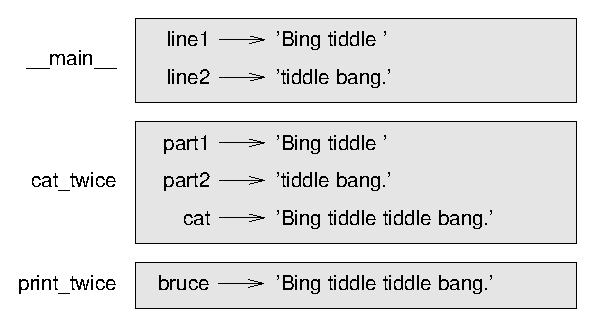
\includegraphics{figs/stack.eps}}
\afterfig

The frames are arranged in a stack that indicates which function
called which, and so on.  In this example, \verb"print_twice"
was called by \verb"cat_twice", and \verb"cat_twice" was called by 
\verb"__main__", which is a special name for the topmost frame.  When
you create a variable outside of any function, it belongs to 
\verb"__main__". Such variable is said to be {\bf global} as opposed to local.

Each parameter refers to the same value as its corresponding
argument.  So, {\tt part1} has the same value as
{\tt line1}, {\tt part2} has the same value as {\tt line2},
and {\tt word} has the same value as {\tt cat}.
If an error occurs during a function call, Python prints the
name of the function, and the name of the function that called
it, and the name of the function that called {\em that}, all the
way back to \verb"__main__".

For example, if you try to access {\tt cat} from within 
\verb"print_twice" -- for example by adding the statement {\tt print(cat)} in the definition of \verb"print_twice" -- you get a {\tt NameError}:

\beforeverb
\begin{pyinterpreter}
Traceback (innermost last):
  File "test.py", line 13, in __main__
    cat_twice(line1, line2)
  File "test.py", line 5, in cat_twice
    print_twice(cat)
  File "test.py", line 9, in print_twice
    print(cat)
NameError: name 'cat' is not defined
\end{pyinterpreter}
\afterverb
%
This list of functions is called a {\bf traceback}.  It tells you what
program file the error occurred in, and what line, and what functions
were executing at the time.  It also shows the line of code that
caused the error.
%
\index{traceback}
%
The order of the functions in the traceback is the same as the
order of the frames in the stack diagram.  The function that is
currently running is at the bottom.


\section{Void functions and non-void functions}

\index{non-void function}
\index{void function}
\index{function, non-void}
\index{function, void} 

Some of the functions we are using, such as the math functions, yield
results; for lack of a better name, we call them {\bf non-void
  functions}.  Other functions, like \verb"print_twice", perform an
action but don't return a value.  They are called {\bf void
  functions}.

When you call a non-void function, you almost always
want to do something with the result; for example, you might
assign it to a variable or use it as part of an expression:

\beforeverb
\begin{pycode}
x = math.cos(radians)
golden = (math.sqrt(5) + 1) / 2
\end{pycode}
\afterverb
%
When you call a function in interactive mode, Python displays
the result:

\beforeverb
\begin{pyinterpreter}
>>> math.sqrt(5)
2.2360679774997898
\end{pyinterpreter}
\afterverb
%
But in a script, if you call a non-void function all by itself,
the return value is lost forever!

\beforeverb
\begin{pyinterpreter}
math.sqrt(5)
\end{pyinterpreter}
\afterverb
%
This script computes the square root of 5, but since it doesn't store
or display the result, it is not very useful.
%
\index{interactive mode}
\index{script mode}
%
Void functions might display something on the screen or have some
other effect, but they don't have a return value.  If you try to
assign the result to a variable, you get a special value called
{\tt None}. Note the capital letter {\tt N} in {\tt None}.

\index{None special value}
\index{special value!None}

\beforeverb
\begin{pyinterpreter}
>>> result = print_twice('Bing')
Bing
Bing
>>> print(result)
None
\end{pyinterpreter}
\afterverb
%
The value {\tt None} is not the same as the string \verb"'None'". 
It is a special value that has its own type:

\beforeverb
\begin{pyinterpreter}
>>> print type(None)
<type 'NoneType'>
\end{pyinterpreter}
\afterverb
%
The functions we have written so far are all void.  We will start
writing non-void functions in a few chapters.


\section{Why functions?}
\index{function, reasons for}

It may not be clear why it is worth the trouble to divide
a program into functions.  There are several reasons:

\begin{itemize}

\item Creating a new function gives you an opportunity to name a group
of statements, which makes your program easier to read and debug.

\item Functions can make a program smaller by eliminating repetitive
code.  Later, if you make a change, you only have
to make it in one place. This make your code easier to maintain.

\item Dividing a long program into functions allows you to debug the
parts one at a time and then assemble them into a working whole.

\item Well-designed functions are often useful for many programs.
Once you write and debug one, you can reuse it. The aim is to write
 code once and use it many times.

\end{itemize}


\section{Debugging}
\label{editor}
\index{debugging}

If you are using a text editor to write your scripts, you might
run into problems with spaces and tabs.  The best way to avoid
these problems is to use spaces exclusively (no tabs).  Most text
editors that know about Python do this by default, but some
don't.
%
\index{whitespace}
%
Tabs and spaces are usually invisible, which makes them
hard to debug, so try to find an editor that manages indentation
for you.
%
Also, don't forget to save your program before you run it.  Some
development environments do this automatically, but some don't.
In that case the program you are looking at in the text editor
is not the same as the program you are running.
%
Debugging can take a long time if you keep running the same,
incorrect, program over and over!
%
Make sure that the code you are looking at is the code you are running.
If you're not sure, put something like \verb"print('hello')" at the
beginning of the program and run it again.  If you don't see
\verb"hello", you're not running the right program!




\section{Glossary}

	
\begin{vocabulary}[function:] A named sequence of statements that performs some
useful operation.  Functions may or may not take arguments and may or
may not produce a result.
\index{function}
\end{vocabulary}
	
\begin{vocabulary}[function definition:]  A statement that creates a new function,
specifying its name, parameters, and the statements it executes.
\index{function definition}
\end{vocabulary}
	
\begin{vocabulary}[function object:]  A value created by a function definition.
The name of the function is a variable that refers to a function
object.
\index{function definition}
\end{vocabulary}
	
\begin{vocabulary}[header:] The first line of a function definition.
\index{header}
\end{vocabulary}
	
\begin{vocabulary}[body:] The sequence of statements inside a function definition.
\index{body}
\end{vocabulary}
	
\begin{vocabulary}[parameter:] A name used inside a function to refer to the value
passed as an argument.
\index{parameter}
\end{vocabulary}
	
\begin{vocabulary}[function call:] A statement that executes a function. It
consists of the function name followed by an argument list.
\index{function call}
\end{vocabulary}
	
\begin{vocabulary}[argument:]  A value provided to a function when the function is called.
This value is assigned to the corresponding parameter in the function.
\index{argument}
\end{vocabulary}
	
\begin{vocabulary}[local variable:]  A variable defined inside a function.  A local
variable can only be used inside its function.
\index{local variable}
\end{vocabulary}
	
\begin{vocabulary}[return value:]  The result of a function.  If a function call
is used as an expression, the return value is the value of
the expression.
\index{return value}
\end{vocabulary}
	
\begin{vocabulary}[non-void function:] A function that returns a value.
\index{non-void function}
\end{vocabulary}
	
\begin{vocabulary}[void function:] A function that doesn't return a value.
\index{void function}
\end{vocabulary}
	
\begin{vocabulary}[module:] A file that contains a
collection of related functions and other definitions.
\index{module}
\end{vocabulary}
	
\begin{vocabulary}[import statement:] A statement that reads a module file and creates
a module object.
\index{import statement}
\index{statement!import}
\end{vocabulary}
	
\begin{vocabulary}[module object:] A value created by an {\tt import} statement
that provides access to the values defined in a module.
\index{module}
\end{vocabulary}
	
\begin{vocabulary}[dot notation:]  The syntax for calling a function in another
module by specifying the module name followed by a dot (period) and
the function name.
\index{dot notation}
\end{vocabulary}
	
\begin{vocabulary}[composition:] Using an expression as part of a larger expression,
or a statement as part of a larger statement.
\index{composition}
\end{vocabulary}
	
\begin{vocabulary}[flow of execution:]  The order in which statements are executed during
a program run.
\index{flow of execution}
\end{vocabulary}
	
\begin{vocabulary}[stack diagram:]  A graphical representation of a stack of functions,
their variables, and the values they refer to.
\index{stack diagram}
\end{vocabulary}
	
\begin{vocabulary}[frame:]  A box in a stack diagram that represents a function call.
It contains the local variables and parameters of the function.
\index{function frame}
\index{frame}
\end{vocabulary}
	
\begin{vocabulary}[traceback:]  A list of the functions that are executing,
printed when an exception occurs.
\index{traceback}
\end{vocabulary}


\section{Exercises}

\begin{exercise}

\index{len function}
\index{function!len}

Python provides a built-in function called {\tt len} that
returns the length of a string, so the value of \verb"len('allen')" is 5.

Write a function named \verb"right_justify" that takes a string
named {\tt s} as a parameter and prints the string with enough
leading spaces so that the last letter of the string is in column 70
of the display.

\beforeverb
\begin{pyexo}
>>> right_justify('allen')
                                                       allen
\end{pyexo}
\afterverb

\end{exercise}


\begin{exercise}
\index{function object}
\index{object!function}

A function object is a value you can assign to a variable
or pass as an argument.  For example, \verb"do_twice" is a function
that takes a function object as an argument and calls it twice:

\beforeverb
\begin{pyexo}
def do_twice(f):
    f()
    f()
\end{pyexo}
\afterverb

Here's an example that uses \verb"do_twice" to call a function
named \verb"print_spam" twice.

\beforeverb
\begin{pyexo}
def print_spam():
    print('spam')

do_twice(print_spam)
\end{pyexo}
\afterverb

\begin{enumerate}

\item Type this example into a script and test it.

\item Modify \verb"do_twice" so that it takes two arguments, a
function object and a value, and calls the function twice,
passing the value as an argument.

\item Write a more general version of \verb"print_spam", called
\verb"print_twice", that takes a string as a parameter and prints
it twice.

\item Use the modified version of \verb"do_twice" to call
\verb"print_twice" twice, passing \verb"'spam'" as an argument.

\item Define a new function called 
\verb"do_four" that takes a function object and a value
and calls the function four times, passing the value
as a parameter.  There should be only
two statements in the body of this function, not four.

\end{enumerate}

{\color{red} You can see my solution at \url{thinkpython.com/code/do_four.py}.}

\end{exercise}



\begin{exercise}
This exercise\footnote{Based on an exercise in Oualline, {\em
    Practical C Programming, Third Edition}, O'Reilly (1997)} can be
done using only the statements and other features we have learned so
far.  

\index{grid}

\begin{enumerate}

\item Write a function that draws a grid like the
  following:

\beforeverb
\begin{pyexo}
+ - + - +
|   |   |
+ - + - +
|   |   |
+ - + - +
\end{pyexo}
\afterverb
%
Hint: to print more than one value on a line, you can print
a comma-separated sequence:

\beforeverb
\begin{pyexo}
print('+', '-')
\end{pyexo}
\afterverb
%
In order to build a string spanning several lines, we can use the string character \verb|'\n'| which represents the newline character. The newline character can be embedded in a string, or can be concatenated using the {\tt +} operator as shown in the following examples.

\beforeverb
\begin{pyexo}
>>> print('line 1 \nline 2')
line 1 
line 2
>>> print('line 1' + '\n' + 'line 2')
line 1
line 2
\end{pyexo}
\afterverb
%
A {\tt print} statement all by itself ends the current line and
goes to the next line.

\item Use the previous function to draw a similar grid
with four rows and four columns.

\end{enumerate}

{\color{red} You can see my solution at \url{thinkpython.com/code/grid.py}.}

\end{exercise}




%
%\chapterimage{chapter_head_1.pdf}
\chapter{Conditionals}

\section{Modulus operator}

\index{modulus operator}
\index{operator!modulus}

The {\bf modulus operator} works on integers and yields the remainder
when the first operand is divided by the second.  In Python, the
modulus operator is a percent sign (\verb"%").  The syntax is the same
as for other operators:

\beforeverb
\begin{pycode}
>>> quotient = 7 // 3
>>> print(quotient)
2
>>> remainder = 7 % 3
>>> print(remainder)
1
\end{pycode}
\afterverb
%
So 7 divided by 3 is 2 with 1 left over.

The modulus operator turns out to be surprisingly useful.  For
example, you can check whether one number is divisible by another---if
{\tt x \% y} is zero, then {\tt x} is divisible by {\tt y}.
%
\index{divisibility}
%
Also, you can extract the right-most digit
or digits from a number.  For example, {\tt x \% 10} yields the
right-most digit of {\tt x} (in base 10).  Similarly {\tt x \% 100}
yields the last two digits.


\section{Boolean expressions}
\index{boolean expression}
\index{expression!boolean}
\index{logical operator}
\index{operator!logical}

A {\bf boolean expression} is an expression that is either true
or false.  The following examples use the 
operator {\tt ==}, which compares two operands and produces
{\tt True} if they are equal and {\tt False} otherwise:

\beforeverb
\begin{pycode}
>>> 5 == 5
True
>>> 5 == 6
False
\end{pycode}
\afterverb
%
{\tt True} and {\tt False} are special
values that belong to the type {\tt bool}; they are not strings:

\index{True special value}
\index{False special value}
\index{special value!True}
\index{special value!False}
\index{bool type}
\index{type!bool}

\beforeverb
\begin{pycode}
>>> type(True)
<type 'bool'>
>>> type(False)
<type 'bool'>
\end{pycode}
\afterverb
%
The {\tt ==} operator is one of the {\bf relational operators}; the
others are:

\beforeverb
\begin{pycode}
x != y               # x is not equal to y
x > y                # x is greater than y
x < y                # x is less than y
x >= y               # x is greater than or equal to y
x <= y               # x is less than or equal to y
\end{pycode}
\afterverb
%
Although these operations are probably familiar to you, the Python
symbols are different from the mathematical symbols.  A common error
is to use a single equal sign ({\tt =}) instead of a double equal sign
({\tt ==}).  Remember that {\tt =} is an assignment operator and
{\tt ==} is a relational operator.   There is no such thing as
{\tt =<} or {\tt =>}.

\index{relational operator}
\index{operator!relational}


\section {Logical operators}
\index{logical operator}
\index{operator!logical}

There are three {\bf logical operators}: {\tt and}, {\tt
or}, and {\tt not}.  The semantics (meaning) of these operators is
similar to their meaning in English. If you are not familiar with the logical operators, their {\bf truth table} are given in Table~\ref{tab:truth_table}. The tables read as follow, the operands value are given in the first row and first column. The operator is given in the first cell (top-left) of the table. Looking at the {\tt and} operator, the result of the expression {\tt True and True} is {\tt True}, whereas the result of the expression {\tt True and False} is {\tt False}.

\begin{table}[htb]
\begin{center}
\begin{minipage}[t]{.3\textwidth}
\begin{tabular}{|c|cc|}
\hline
and   & True  & False \\\hline
True  & True  & False \\
False & False & False \\\hline
\end{tabular}
\end{minipage}
%
\begin{minipage}[t]{.3\textwidth}
\begin{tabular}{|c|cc|}
\hline
or    & True  & False \\\hline
True  & True  & True  \\
False & True  & False \\\hline
\end{tabular}
\end{minipage}
%
\begin{minipage}[t]{.3\textwidth}
\begin{tabular}{|c|cc|}
\hline
not  & True  & False\\\hline
     & False & True \\\hline
\end{tabular}
\end{minipage}
%
\caption{Truth table for the three logical operators {\tt and}, {\tt or}, and {\tt not}.}
\label{tab:truth_table}
\end{center}
\end{table}

%
\index{and operator}
\index{or operator}
\index{not operator}
\index{operator!and}
\index{operator!or}
\index{operator!not}
\index{operator!truth table}

%
 For example, {\tt x > 0 and x < 10} is true only if {\tt x} is greater than 0
{\em and} less than 10. Another example, {\tt n\%2 == 0 or n\%3 == 0} is true if {\em either} of the conditions
is true, that is, if the number is divisible by 2 {\em or} 3.
%
Finally, the {\tt not} operator negates a Boolean
expression, so {\tt not (x > y)} is true if {\tt x > y} is false,
that is, if {\tt x} is less than or equal to {\tt y}.

\begin{remark}
Strictly speaking, the operands of the logical operators should be
Boolean expressions, but Python is not very strict.
Any nonzero number is interpreted as ``true'', wheres as 0 is interpreted as ``false''.

\beforeverb
\begin{pycode}
>>> 17 and True
True
\end{pycode}
\afterverb
%
This flexibility can be useful, but there are some subtleties to
it that might be confusing.  You might want to (shall I say MUST) avoid it, even if
you know what you are doing. Another developer maintaining your code may not be familiar with the subtleties.

\end{remark}


\section{Conditional execution}
\label{conditional execution}

\index{conditional statement}
\index{statement!conditional}
\index{if statement}
\index{statement!if}
\index{conditional execution}

In order to write useful programs, we almost always need the ability
to check conditions and change the behavior of the program
accordingly.  {\bf Conditional statements} give us this ability.  The
simplest form is the {\tt if} statement:

\beforeverb
\begin{pycode}
if x > 0:
    print('x is positive')
\end{pycode}
\afterverb
%
The Boolean expression after the {\tt if} statement is
called the {\bf condition}.  If it is true, then the indented
statement gets executed.  If not, nothing happens.

\index{condition}
\index{compound statement}
\index{statement!compound}

{\tt if} statements have the same structure as function definitions:
a header followed by an indented body.  Statements like this are
called {\bf compound statements}.
%
There is no limit on the number of statements that can appear in
the body, but there has to be at least one.
Occasionally, it is useful to have a body with no statements (usually
as a place keeper for code you haven't written yet).  In that
case, you can use the {\tt pass} statement, which does nothing.

\index{pass statement}
\index{statement!pass}

\beforeverb
\begin{pycode}
if x < 0:
    pass          # need to handle negative values!
\end{pycode}
\afterverb
%

\section{Alternative execution}
\label{alternative execution}

\index{alternative execution}
\index{else keyword}
\index{keyword!else}

A second form of the {\tt if} statement is {\bf alternative execution} (aka {\tt if-else} statement),
in which there are two possibilities and the condition determines
which one gets executed.  The syntax looks like this:

\beforeverb
\begin{pycode}
if x%2 == 0:
    print('x is even')
else:
    print('x is odd')
\end{pycode}
\afterverb
%
If the remainder when {\tt x} is divided by 2 is 0, then we
know that {\tt x} is even, and the program displays a message to that
effect.  If the condition is false, the second set of statements is
executed.  Since the condition must be true or false, exactly one of
the alternatives will be executed.  The alternatives are called
{\bf branches}, because they are branches in the flow of execution.

\index{branch}



\section{Chained conditionals}
\index{chained conditional}
\index{conditional!chained}

Sometimes there are more than two possibilities and we need more than
two branches.  One way to express a computation like that is a {\bf
chained conditional} (aka {\tt if-elif-else} statement):

\beforeverb
\begin{pycode}
if x < y:
    print('x is less than y')
elif x > y:
    print('x is greater than y')
else:
    print('x and y are equal')
\end{pycode}
\afterverb
%
{\tt elif} is an abbreviation of ``else if.''  Again, exactly one
branch will be executed.  There is no limit on the number of {\tt
elif} statements.  If there is an {\tt else} clause, it has to be
at the end, but there doesn't have to be one.

\index{elif keyword}
\index{keyword!elif}


\beforeverb
\begin{pycode}
if choice == 'a':
    draw_a()
elif choice == 'b':
    draw_b()
elif choice == 'c':
    draw_c()
\end{pycode}
\afterverb
%
Each condition is checked in order.  If the first is false,
the next is checked, and so on.  If one of them is
true, the corresponding branch executes, and the statement
ends.  Even if more than one condition is true, only the
first true branch executes.  


\section{Nested conditionals}
\index{nested conditional}
\index{conditional!nested}

One conditional can also be nested within another.  We could have
written the trichotomy example like this:

\beforeverb
\begin{pycode}
if x == y:
    print('x and y are equal')
else:
    if x < y:
        print('x is less than y')
    else:
        print('x is greater than y')
\end{pycode}
\afterverb
%
The outer conditional contains two branches.  The
first branch contains a simple statement.  The second branch
contains another {\tt if} statement, which has two branches of its
own.  Those two branches are both simple statements,
although they could have been conditional statements as well.
%
Although the indentation of the statements makes the structure
apparent, {\bf nested conditionals} become difficult to read very
quickly. In general, it is a good idea to avoid them when you can.

Logical operators often provide a way to simplify nested conditional
statements.  For example, we can rewrite the following code using a
single conditional:

\beforeverb
\begin{pycode}
if 0 < x:
    if x < 10:
        print('x is a positive single-digit number.')
\end{pycode}
\afterverb
%
The {\tt print} statement is executed only if we make it past both
conditionals, so we can get the same effect with the {\tt and} operator:

\beforeverb
\begin{pycode}
if 0 < x and x < 10:
    print('x is a positive single-digit number.')
\end{pycode}
\afterverb		



%
%\chapterimage{chapter_head_1.pdf}
\chapter{Iteration}
\index{iteration}


\section{Multiple assignment}

\index{assignment}
\index{statement!assignment}
\index{multiple assignment}

As you may have discovered, it is legal to
make more than one assignment to the same variable.  A
new assignment makes an existing variable refer to a new
value (and stop referring to the old value).

\beforeverb
\begin{pycode}
bruce = 5
print(bruce)
bruce = 7
print(bruce)
\end{pycode}
\afterverb
%
The output of this program is:
\beforeverb
\begin{pycode}
5
7
\end{pycode}
\afterverb
%
because the first time {\tt bruce} is printed, its value is 5, and the second time, its
value is 7.  Here is what {\bf multiple assignment} looks like in a state diagram:

\index{state diagram}
\index{diagram!state}

\beforefig
\centerline{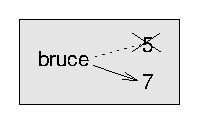
\includegraphics{figs/assign2.eps}}
\afterfig

With multiple assignment it is especially important to distinguish
between an assignment operation and a statement of equality.  Because
Python uses the equal sign ({\tt =}) for assignment, it is tempting to
interpret a statement like {\tt a = b} as a statement of equality. It
is not!

\index{equality and assignment}

First, equality is a symmetric relation and assignment is not.  For
example, in mathematics, if $a = 7$ then $7 = a$.  But in Python, the
statement {\tt a = 7} is legal and {\tt 7 = a} is not.
%
Furthermore, in mathematics, a statement of equality is either true or
false, for all time.  If $a = b$ now, then $a$ will always equal $b$.
In Python, an assignment statement can make two variables equal, but
they don't have to stay that way:

\beforeverb
\begin{pycode}
a = 5
b = a    # a and b are now equal
a = 3    # a and b are no longer equal
\end{pycode}
\afterverb
%
The third line changes the value of {\tt a} but does not change the
value of {\tt b}, so they are no longer equal. 
%
Although multiple assignment is frequently helpful, you should use it
with caution.  If the values of variables change frequently, it can
make the code difficult to read and debug.


\section{Updating variables}
\label{update}

\index{update}
\index{variable!updating}

One of the most common forms of multiple assignment is an {\bf update},
where the new value of the variable depends on the old.

\beforeverb
\begin{pycode}
x = x+1
\end{pycode}
\afterverb
%
This means ``get the current value of {\tt x}, add one, and then
update {\tt x} with the new value.''
%
If you try to update a variable that doesn't exist, you get an
error, because Python evaluates the right side before it assigns
a value to {\tt x}:

\beforeverb
\begin{pycode}
>>> y = y+1
Traceback (most recent call last):
  File "<pyshell#49>", line 1, in <module>
    y = y+1
NameError: name 'y' is not defined
\end{pycode}
\afterverb
%
Before you can update a variable, you have to {\bf initialize}
it, usually with a simple assignment:

\index{initialization (before update)}

\beforeverb
\begin{pycode}
>>> y = 0
>>> y = y+1
\end{pycode}
\afterverb
%
Updating a variable by adding 1 is called an {\bf increment};
subtracting 1 is called a {\bf decrement}.

\index{increment}
\index{decrement}




\section{The {\tt while} statement}

\index{statement!while}
\index{while loop}
\index{loop!while}
\index{iteration}

Computers are often used to automate repetitive tasks.  Repeating
identical or similar tasks without making errors is something that
computers do well and people do poorly.

{\color{red} We have seen two programs, {\tt countdown} and \verb"print_n", that
use recursion to perform repetition, which is also called {\bf
iteration}.}
Because iteration is so common, Python provides several
language features to make it easier.  {\color{red} One is the {\tt for} statement
we saw in Section~\ref{repetition}.  We'll get back to that later.}

Another is the {\tt while} statement.  Here is a version of {\tt
countdown} that uses a {\tt while} statement:

\beforeverb
\begin{pycode}
def countdown(n):
    while n > 0:
        print(n)
        n = n-1
    print('Blastoff!')
\end{pycode}
\afterverb
%
You can almost read the {\tt while} statement as if it were English.
It means, ``While {\tt n} is greater than 0,
display the value of {\tt n} and then reduce the value of
{\tt n} by 1.  When you get to 0, display the word {\tt Blastoff!}''

\index{flow of execution}

More formally, here is the flow of execution for a {\tt while} statement:

\begin{enumerate}

\item Evaluate the condition, yielding {\tt True} or {\tt False}.

\item If the condition is false, exit the {\tt while} statement
and continue execution at the next statement.

\item If the condition is true, execute the
body and then go back to step 1.

\end{enumerate}

This type of flow is called a {\bf loop} because the third step
loops back around to the top.  

\index{condition}
\index{loop}
\index{body}

The body of the loop should change the value of one or more variables
so that eventually the condition becomes false and the loop
terminates.  Otherwise the loop will repeat forever, which is called
an {\bf infinite loop}.  An endless source of amusement for computer
scientists is the observation that the directions on shampoo,
``Lather, rinse, repeat,'' are an infinite loop.

\index{infinite loop}
\index{loop!infinite}

In the case of {\tt countdown}, we can prove that the loop
terminates because we know that the value of {\tt n} is finite, and we
can see that the value of {\tt n} gets smaller each time through the
loop, so eventually we have to get to 0.  In other
cases, it is not so easy to tell:

\beforeverb
\begin{pycode}
def sequence(n):
    while n != 1:
        print(n)
        if n % 2 == 0:        # n is even
            n = n / 2
        else:               # n is odd
            n = n * 3 + 1
\end{pycode}
\afterverb
%
The condition for this loop is {\tt n != 1}, so the loop will continue
until {\tt n} is {\tt 1}, which makes the condition false.
%
Each time through the loop, the program outputs the value of {\tt n}
and then checks whether it is even or odd.  If it is even, {\tt n} is 
divided by 2.  If it is odd, the value of {\tt n} is replaced with
{\tt n*3+1}. For example, if the argument passed
to {\tt sequence} is 3, the resulting sequence is 3, 10, 5, 16, 8, 4, 2, 1.

Since {\tt n} sometimes increases and sometimes decreases, there is no
obvious proof that {\tt n} will ever reach 1, or that the program
terminates.  For some particular values of {\tt n}, we can prove
termination.  For example, if the starting value is a power of two,
then the value of {\tt n} will be even each time through the loop
until it reaches 1. The previous example ends with such a sequence,
starting with 16.

\index{Collatz conjecture}

The hard question is whether we can prove that this program terminates
for {\em all positive values} of {\tt n}.  So far\footnote{See
  \url{wikipedia.org/wiki/Collatz_conjecture}.}, no one has
been able to prove it {\em or} disprove it!

\begin{exercise}
\color{red}
Rewrite the function \verb"print_n" from
Section~\ref{recursion} using iteration instead of recursion.
\end{exercise}


\section{{\tt break}}
\index{break statement}
\index{statement!break}

Sometimes you don't know it's time to end a loop until you get half
way through the body.  In that case you can use the {\tt break}
statement to jump out of the loop.

For example, suppose you want to take input from the user until they
type {\tt done}.  You could write:

\beforeverb
\begin{pycode}
while True:
    line = input('> ')
    if line == 'done':
        break
    print(line)

print('Done!')
\end{pycode}
\afterverb
%
The loop condition is {\tt True}, which is always true, so the
loop runs until it hits the break statement.

Each time through, it prompts the user with an angle bracket.
If the user types {\tt done}, the {\tt break} statement exits
the loop.  Otherwise the program echoes whatever the user types
and goes back to the top of the loop.  Here's a sample run:

\beforeverb
\begin{pycode}
> not done
not done
> done
Done!
\end{pycode}
\afterverb
%
This way of writing {\tt while} loops is common because you
can check the condition anywhere in the loop (not just at the
top) and you can express the stop condition affirmatively
(``stop when this happens'') rather than negatively (``keep going
until that happens.'').


\section{Square roots}

\index{square root}

Loops are often used in programs that compute
numerical results by starting with an approximate answer and
iteratively improving it.
%
\index{Newton's method}
%
For example, one way of computing square roots is Newton's method.
Suppose that you want to know the square root of $a$.  If you start
with almost any estimate, $x$, you can compute a better
estimate with the following formula:

\[ y = \frac{x + a/x}{2} \]
%
For example, if $a$ is 4 and $x$ is 3:

\beforeverb
\begin{pycode}
>>> a = 4.0
>>> x = 3.0
>>> y = (x + a/x) / 2
>>> print(y)
2.16666666667
\end{pycode}
\afterverb
%
Which is closer to the correct answer ($\sqrt{4} = 2$).  If we
repeat the process with the new estimate, it gets even closer:

\beforeverb
\begin{pycode}
>>> x = y
>>> y = (x + a/x) / 2
>>> print(y)
2.00641025641
\end{pycode}
\afterverb
%
After a few more updates, the estimate is almost exact:

\index{update}

\beforeverb
\begin{pycode}
>>> x = y
>>> y = (x + a/x) / 2
>>> print(y)
2.00001024003
>>> x = y
>>> y = (x + a/x) / 2
>>> print(y)
2.00000000003
\end{pycode}
\afterverb
%
In general we don't know ahead of time how many steps it takes
to get to the right answer, but we know when we get there
because the estimate
stops changing:

\beforeverb
\begin{pycode}
>>> x = y
>>> y = (x + a/x) / 2
>>> print(y)
2.0
>>> x = y
>>> y = (x + a/x) / 2
>>> print(y)
2.0
\end{pycode}
\afterverb
%
When {\tt y == x}, we can stop.  Here is a loop that starts
with an initial estimate, {\tt x}, and improves it until it
stops changing:

\beforeverb
\begin{pycode}
while True:
    print(x)
    y = (x + a/x) / 2
    if y == x:
        break
    x = y
\end{pycode}
\afterverb
%
For most values of {\tt a} this works fine, but in general it is
dangerous to test {\tt float} equality.
Floating-point values are only approximately right:
most rational numbers, like $1/3$, and irrational numbers, like
$\sqrt{2}$, can't be represented exactly with a {\tt float}.
%
\index{floating-point}
\index{epsilon}
%
Rather than checking whether {\tt x} and {\tt y} are exactly equal, it
is safer to use the built-in function {\tt abs} to compute the
absolute value, or magnitude, of the difference between them:

\beforeverb
\begin{pycode}
    if abs(y-x) < epsilon:
        break
\end{pycode}
\afterverb
%
Where \verb"epsilon" has a value like {\tt 0.0000001} that
determines how close is close enough.
%
\begin{exercise}
\label{square_root}
\index{encapsulation}
%
{\color{red} Encapsulate} this loop in a function called \verb"square_root"
that takes {\tt a} as a parameter, chooses a reasonable
value of {\tt x}, and returns an estimate of the square root
of {\tt a}.
\end{exercise}


\section{Algorithms}
\index{algorithm}

Newton's method is an example of an {\bf algorithm}: it is a
mechanical process for solving a category of problems (in this
case, computing square roots).
%
It is not easy to define an algorithm.  It might help to start
with something that is not an algorithm.  When you learned
to multiply single-digit numbers, you probably memorized the
multiplication table.  In effect, you memorized 100 specific solutions.
That kind of knowledge is not algorithmic.
%
But if you were ``lazy,'' you probably cheated by learning a few
tricks.  For example, to find the product of $n$ and 9, you can
write $n-1$ as the first digit and $10-n$ as the second
digit.  This trick is a general solution for multiplying any
single-digit number by 9.  That's an algorithm!

\index{addition with carrying}
\index{carrying, addition with}
\index{subtraction!with borrowing}
\index{borrowing, subtraction with}

Similarly, the techniques you learned for addition with carrying,
subtraction with borrowing, and long division are all algorithms.  One
of the characteristics of algorithms is that they do not require any
intelligence to carry out.  They are mechanical processes in which
each step follows from the last according to a simple set of rules.

On the other hand, the process of designing algorithms is interesting,
intellectually challenging, and a central part of what we call
programming.
%
Some of the things that people do naturally, without difficulty or
conscious thought, are the hardest to express algorithmically.
Understanding natural language is a good example.  We all do it, but
so far no one has been able to explain {\em how} we do it, at least
not in the form of an algorithm.


\section{Debugging}

As you start writing bigger programs, you might find yourself
spending more time debugging.  More code means more chances to
make an error and more place for bugs to hide.
%
\index{debugging!by bisection}
\index{bisection, debugging by}

One way to cut your debugging time is ``debugging by bisection.''
For example, if there are 100 lines in your program and you
check them one at a time, it would take 100 steps.
%
Instead, try to break the problem in half.  Look at the middle
of the program, or near it, for an intermediate value you
can check.  Add a {\tt print} statement (or something else
that has a verifiable effect) and run the program.
%
If the mid-point check is incorrect, there must be a problem in the
first half of the program.  If it is correct, the problem is
in the second half.
%
Every time you perform a check like this, you halve the number of
lines you have to search.  After six steps (which is fewer than 100),
you would be down to one or two lines of code, at least in theory.

In practice it is not always clear what
the ``middle of the program'' is and not always possible to
check it.  It doesn't make sense to count lines and find the
exact midpoint.  Instead, think about places
in the program where there might be errors and places where it
is easy to put a check.  Then choose a spot where you
think the chances are about the same that the bug is before
or after the check.




\section{Glossary}

\begin{vocabulary}[multiple assignment:] Making more than one assignment to the same
variable during the execution of a program.
\index{multiple assignment}
\index{assignment!multiple}
\end{vocabulary}
	
\begin{vocabulary}[update:] An assignment where the new value of the variable
depends on the old.
\index{update}
\end{vocabulary}
	
\begin{vocabulary}[initialization:] An assignment that gives an initial value to
a variable that will be updated.
\index{initialization!variable}
\end{vocabulary}
	
\begin{vocabulary}[increment:] An update that increases the value of a variable
(often by one).
\index{increment}
\end{vocabulary}
	
\begin{vocabulary}[decrement:] An update that decreases the value of a variable.
\index{decrement}
\end{vocabulary}
	
\begin{vocabulary}[iteration:] Repeated execution of a set of statements using
either a recursive function call or a loop.
\index{iteration}
\end{vocabulary}
	
\begin{vocabulary}[infinite loop:] A loop in which the terminating condition is
never satisfied.
\index{infinite loop}
\end{vocabulary}


\section{Exercises}

\begin{exercise}

\index{algorithm!square root}

To test the square root algorithm in this chapter, you could compare
it with {\tt math.sqrt}.  Write a function named \verb"test_square_root"
that prints a table like this:

\beforeverb
\begin{verbatim}
1.0 1.0           1.0           0.0
2.0 1.41421356237 1.41421356237 2.22044604925e-16
3.0 1.73205080757 1.73205080757 0.0
4.0 2.0           2.0           0.0
5.0 2.2360679775  2.2360679775  0.0
6.0 2.44948974278 2.44948974278 0.0
7.0 2.64575131106 2.64575131106 0.0
8.0 2.82842712475 2.82842712475 4.4408920985e-16
9.0 3.0           3.0           0.0

\end{verbatim}
\afterverb
%
The first column is a number, $a$; the second column is
the square root of $a$ computed with the function from
Exercise~\ref{square_root}; the third column is the square root computed
by {\tt math.sqrt}; the fourth column is the absolute value
of the difference between the two estimates.
\end{exercise}


\begin{exercise}

\index{eval function}
\index{function!eval}

The built-in function {\tt eval} takes a string and evaluates
it using the Python interpreter.  For example:

\beforeverb
\begin{pycode}
>>> eval('1 + 2 * 3')
7
>>> import math
>>> eval('math.sqrt(5)')
2.2360679774997898
>>> eval('type(math.pi)')
<type 'float'>
\end{pycode}
\afterverb
%
Write a function called \verb"eval_loop" that iteratively
prompts the user, takes the resulting input and evaluates
it using {\tt eval}, and prints the result.

It should continue until the user enters \verb"'done'", and then
return the value of the last expression it evaluated.

\end{exercise}


\begin{exercise}

\index{Ramanujan, Srinivasa}

The brilliant mathematician Srinivasa Ramanujan found an
infinite series\footnote{See \url{wikipedia.org/wiki/Pi}.}
that can be used to generate a numerical
approximation of $\pi$:

\index{pi}

\[\frac{1}{\pi} = \frac{2\sqrt{2}}{9801} 
\sum^\infty_{k=0} \frac{(4k)!(1103+26390k)}{(k!)^4 396^{4k}} \]

Write a function called \verb"estimate_pi" that uses this formula
to compute and return an estimate of $\pi$.  It should use a {\tt while}
loop to compute terms of the summation until the last term is
smaller than {\tt 1e-15} (which is Python notation for $10^{-15}$).
You can check the result by comparing it to {\tt math.pi}.

You can see my solution at \url{thinkpython.com/code/pi.py}.
\end{exercise}


%\part{Part II}

%\chapterimage{chapter_head_1.pdf}
\chapter{Strings}
\label{strings}


\section{A string is a sequence}
\index{sequence}
\index{character}
\index{bracket operator}
\index{operator!bracket}

A string is a {\bf sequence} of characters.  
You can access the characters one at a time with the
bracket operator:

\beforeverb
\begin{pyinterpreter}
>>> fruit = 'banana'
>>> letter = fruit[1]
\end{pyinterpreter}
\afterverb
%
The second statement selects character number 1 from {\tt
fruit} and assigns it to {\tt letter}.  
%
\index{index}
%
The expression in brackets is called an {\bf index}.  
The index indicates which character in the sequence you
want (hence the name).
%
But you might not get what you expect:

\beforeverb
\begin{pyinterpreter}
>>> print(letter)
a
\end{pyinterpreter}
\afterverb
%
For most people, the first letter of \verb"'banana'" is {\tt b}, not
{\tt a}.  But for computer scientists, the index is an offset from the
beginning of the string, and the offset of the first letter is zero.

\beforeverb
\begin{pyinterpreter}
>>> letter = fruit[0]
>>> print(letter)
b
\end{pyinterpreter}
\afterverb
%
So {\tt b} is the 0th letter (``zero-eth'') of \verb"'banana'", {\tt a}
is the 1th letter (``one-eth''), and {\tt n} is the 2th (``two-eth'')
letter.

\index{index!starting at zero}
\index{zero, index starting at}

You can use any expression, including variables and operators, as an
index, but the value of the index has to be an integer.  Otherwise you
get:

\index{index}
\index{exception!TypeError}
\index{TypeError}

\beforeverb
\begin{pyinterpreter}
>>> letter = fruit[1.5]
TypeError: string indices must be integers
\end{pyinterpreter}
\afterverb
%

\section{Function {\tt len}}

\index{len function}
\index{function!len}

{\tt len} is a built-in function that returns the number of characters
in a string:

\beforeverb
\begin{pyinterpreter}
>>> fruit = 'banana'
>>> len(fruit)
6
\end{pyinterpreter}
\afterverb
%
To get the last letter of a string, you might be tempted to try something
like this:

\index{exception!IndexError}
\index{IndexError}

\beforeverb
\begin{pyinterpreter}
>>> length = len(fruit)
>>> last = fruit[length]
IndexError: string index out of range
\end{pyinterpreter}
\afterverb
%
The reason for the {\tt IndexError} is that there is no letter in {\tt
'banana'} with the index 6.  Since we started counting at zero, the
six letters are numbered 0 to 5.  To get the last character, you have
to subtract 1 from {\tt length}:

\beforeverb
\begin{pyinterpreter}
>>> last = fruit[length-1]
>>> print(last)
a
\end{pyinterpreter}
\afterverb
%
Alternatively, you can use negative indices, which count backward from
the end of the string.  The expression {\tt fruit[-1]} yields the last
letter, {\tt fruit[-2]} yields the second to last, and so on.

\index{index!negative}
\index{negative index}


\section{Traversal with a {\tt for} loop}
\label{for}

\index{traversal}
\index{loop!traversal}
\index{for loop}
\index{loop!for}
\index{statement!for}
\index{traversal}

A lot of computations involve processing a string one character at a
time.  Often they start at the beginning, select each character in
turn, do something to it, and continue until the end.  This pattern of
processing is called a {\bf traversal}.  One way to write a traversal
is with a {\tt while} loop:

\beforeverb
\begin{pycode}
index = 0
while index < len(fruit):
    letter = fruit[index]
    print(letter)
    index = index + 1
\end{pycode}
\afterverb
%
This loop traverses the string and displays each letter on a line by
itself.  The loop condition is {\pyinline/index < len(fruit)/}, so
when {\tt index} is equal to the length of the string, the
condition is false, and the body of the loop is not executed.  The
last character accessed is the one with the index {\tt len(fruit)-1},
which is the last character in the string.

\begin{exercise}
Write a function that takes a string as an argument
and displays the letters backward, one per line.
\end{exercise}

Another way to write a traversal is with a {\tt for} loop:

\beforeverb
\begin{pycode}
for char in fruit:
    print(char)
\end{pycode}
\afterverb
%
Each time through the loop, the next character in the string is assigned
to the variable {\tt char}.  The loop continues until no characters are
left.

\index{concatenation}
\index{abecedarian}
\index{McCloskey, Robert}

The following example shows how to use concatenation (string addition)
and a {\tt for} loop to generate an abecedarian series (that is, in
alphabetical order).  In Robert McCloskey's book {\em Make
Way for Ducklings}, the names of the ducklings are Jack, Kack, Lack,
Mack, Nack, Ouack, Pack, and Quack.  This loop outputs these names in
order:

\beforeverb
\begin{pycode}
prefixes = 'JKLMNOPQ'
suffix = 'ack'

for letter in prefixes:
    print(letter + suffix)
\end{pycode}
\afterverb
%
The output is:

\beforeverb
\begin{pyoutput}
Jack
Kack
Lack
Mack
Nack
Oack
Pack
Qack
\end{pyoutput}
\afterverb
%
Of course, that's not quite right because ``Ouack'' and
``Quack'' are misspelled.

\begin{exercise}
Modify the program to fix this error.
\end{exercise}



\section{String slices}
\label{slice}

\index{slice operator}
\index{operator!slice}
\index{index!slice}
\index{string!slice}
\index{slice!string}

A segment of a string is called a {\bf slice}.  Selecting a slice is
similar to selecting a character:

\beforeverb
\begin{pyinterpreter}
>>> s = 'Monty Python'
>>> print(s[0:5])
Monty
>>> print(s[6:12])
Python
\end{pyinterpreter}
\afterverb
%
The operator {\pyinline/[n:m]/} returns the part of the string from the 
``n-eth'' character to the ``m-eth'' character, including the first but
excluding the last.  This behavior is counter intuitive, but it might
help to imagine the indices pointing {\em between} the
characters, as in the following diagram:

\beforefig
\centerline{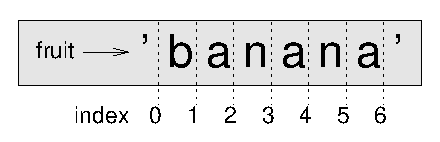
\includegraphics{figs/banana.eps}}
\afterfig

If you omit the first index (before the colon), the slice starts at
the beginning of the string.  If you omit the second index, the slice
goes to the end of the string:

\beforeverb
\begin{pyinterpreter}
>>> fruit = 'banana'
>>> fruit[:2]
'bana'
>>> fruit[2:]
'nana'
\end{pyinterpreter}
\afterverb
%
If the first index is greater than or equal to the second the result
is an {\bf empty string}, represented by two quotation marks:

\index{quotation mark}

\beforeverb
\begin{pyinterpreter}
>>> fruit = 'banana'
>>> fruit[3:3]
''
\end{pyinterpreter}
\afterverb
%
An empty string contains no characters and has length 0, but other
than that, it is the same as any other string.

\begin{exercise}
Given that {\tt fruit} is a string, what does
{\tt fruit[:]} mean?

\index{copy!slice}
\index{slice!copy}


\end{exercise}


\section{Strings are immutable}
\index{mutability}
\index{immutability}
\index{string!immutable}

It is tempting to use the {\tt [ ]} operator on the left side of an
assignment, with the intention of changing a character in a string.
For example:

\index{TypeError}
\index{exception!TypeError}

\beforeverb
\begin{pyinterpreter}
>>> greeting = 'Hello, world!'
>>> greeting[0] = 'J'
TypeError: object does not support item assignment
\end{pyinterpreter}
\afterverb
%
The ``object'' in this case is the string and the ``item'' is
the character you tried to assign.  For now, an {\bf object} is
the same thing as a value, but we will refine that definition
later.  An {\bf item} is one of the values in a sequence.
%
\index{object}
\index{item assignment}
\index{assignment!item}
\index{immutability}
%
The reason for the error is that
strings are {\bf immutable}, which means you can't change an
existing string.  The best you can do is create a new string
that is a variation on the original:

\beforeverb
\begin{pyinterpreter}
>>> greeting = 'Hello, world!'
>>> new_greeting = 'J' + greeting[1:]
>>> print(new_greeting)
Jello, world!
\end{pyinterpreter}
\afterverb
%
This example concatenates a new first letter onto
a slice of {\tt greeting}.  It has no effect on
the original string.

\index{concatenation}


\section{Searching}
\label{find}

What does the following function do?

\index{find function}
\index{function!find}

\beforeverb
\begin{pycode}
def find(word, letter):
    index = 0
    while index < len(word):
        if word[index] == letter:
            return index
        index = index + 1
    return -1
\end{pycode}
\afterverb
%
In a sense, {\tt find} is the opposite of the {\tt [ ]} operator.
Instead of taking an index and extracting the corresponding character,
it takes a character and finds the index where that character
appears.  If the character is not found, the function returns {\tt
-1}.
%
This is the first example we have seen of a {\tt return} statement
inside a loop.  If {\tt word[index] == letter}, the function breaks
out of the loop and returns immediately.
%
If the character doesn't appear in the string, the program
exits the loop normally and  returns {\tt -1}.
%
This pattern of computation---traversing a sequence and returning
when we find what we are looking for---is called a {\bf search}.

\index{traversal}
\index{search pattern}
\index{pattern!search}

\begin{exercise}
Modify {\tt find} so that it has a
third parameter, the index in {\tt word} where it should start
looking.
\end{exercise}


\section{Looping and counting}
\label{counter}

\index{counter}
\index{counting and looping}
\index{looping and counting}
\index{looping!with strings}

The following program counts the number of times the letter {\tt a}
appears in a string:

\beforeverb
\begin{pycode}
word = 'banana'
count = 0
for letter in word:
    if letter == 'a':
        count = count + 1
print(count)
\end{pycode}
\afterverb
%
This program demonstrates another pattern of computation called a {\bf
counter}.  The variable {\tt count} is initialized to 0 and then
incremented each time an {\tt a} is found.
When the loop exits, {\tt count}
contains the result---the total number of {\tt a}'s.

\begin{exercise}
\index{encapsulation}

Encapsulate this code in a function named {\tt
count}, and generalize it so that it accepts the string and the
letter as arguments.
\end{exercise}

\begin{exercise}
Rewrite this function so that instead of
traversing the string, it uses the three-parameter version of {\tt
find} from the previous section.
\end{exercise}


\section{{\tt string} methods}

A {\bf method} is similar to a function---it takes arguments and
may return a value---but the syntax is different.  For example, the
method {\tt upper} takes a string and returns a new string with
all uppercase letters:
%
\index{method}
\index{string!method}
%
Instead of the function syntax {\tt upper(word)}, it uses
the method syntax {\tt word.upper()}.

\index{dot notation}

\beforeverb
\begin{pyinterpreter}
>>> word = 'banana'
>>> new_word = word.upper()
>>> print(new_word)
BANANA
\end{pyinterpreter}
\afterverb
%
This form of dot notation specifies the name of the method, {\tt
upper}, and the name of the string to apply the method to, {\tt
word}.  The empty parentheses indicate that this method takes no
argument.

\index{parentheses!empty}

A method call is called an {\bf invocation}; in this case, we would
say that we are invoking {\tt upper} on the {\tt word}.
%
\index{invocation}
%
As it turns out, there is a string method named {\tt find} that
is remarkably similar to the function we wrote:

\beforeverb
\begin{pyinterpreter}
>>> word = 'banana'
>>> index = word.find('a')
>>> print(index)
1
\end{pyinterpreter}
\afterverb
%
In this example, we invoke {\tt find} on {\tt word} and pass
the letter we are looking for as a parameter.
%
Actually, the {\tt find} method is more general than our function;
it can find substrings, not just characters:

\beforeverb
\begin{pyinterpreter}
>>> word.find('na')
2
\end{pyinterpreter}
\afterverb
%
It can take as a second argument the index where it should start:

\index{optional argument}
\index{argument!optional}

\beforeverb
\begin{pyinterpreter}
>>> word.find('na', 3)
4
\end{pyinterpreter}
\afterverb
%
And as a third argument the index where it should stop:

\beforeverb
\begin{pyinterpreter}
>>> name = 'bob'
>>> name.find('b', 1, 2)
-1
\end{pyinterpreter}
\afterverb
%
This search fails because {\tt b} does not
appear in the index range from {\tt 1} to {\tt 2} (not including {\tt
2}).


\begin{exercise}
\index{count method}
\index{method!count}

There is a string method called {\tt count} that is similar
to the function in the previous exercise.  Read the documentation
of this method
and write an invocation that counts the number of {\tt a}
in \verb"'banana'".
\end{exercise}


\section{The {\tt in} operator}
\label{inboth}

\index{in operator}
\index{operator!in}
\index{boolean operator}
\index{operator!boolean}

The word {\tt in} is a boolean operator that takes two strings and
returns {\tt True} if the first appears as a substring in the second:

\beforeverb
\begin{pyinterpreter}
>>> 'ana' in 'banana'
True
>>> 'rama' in 'banana'
False
\end{pyinterpreter}
\afterverb
%
For example, the following function prints all the
letters from {\tt word1} that also appear in {\tt word2}:

\beforeverb
\begin{pycode}
def in_both(word1, word2):
    for letter in word1:
        if letter in word2:
            print(letter)
\end{pycode}
\afterverb
%
With well-chosen variable names,
Python sometimes reads like English.  You could read
this loop, ``for (each) letter in (the first) word, if (the) letter 
(appears) in (the second) word, print (the) letter.''

Here's what you get if you compare apples and oranges:

\beforeverb
\begin{pyinterpreter}
>>> in_both('apples', 'oranges')
a
e
s
\end{pyinterpreter}
\afterverb
%

\section{String comparison}

\index{string!comparison}
\index{comparison!string}

The relational operators work on strings.  To see if two strings are equal:

\beforeverb
\begin{pycode}
if word == 'banana':
    print ('All right, bananas.')
\end{pycode}
\afterverb
%
Other relational operations are useful for putting words in alphabetical
order:

\beforeverb
\begin{pycode}
if word < 'banana':
    print('Your word,' + word + ', comes before banana.')
elif word > 'banana':
    print('Your word,' + word + ', comes after banana.')
else:
    print('All right, bananas.')
\end{pycode}
\afterverb
%
%Python does not handle uppercase and lowercase letters the same way
%that people do.  All the uppercase letters come before all the
%lowercase letters, so:
%
%\beforeverb
%\begin{pycode}
%Your word, Pineapple, comes before banana.
%\end{pycode}
%\afterverb
%%
%A common way to address this problem is to convert strings to a
%standard format, such as all lowercase, before performing the
%comparison.  Keep that in mind in case you have to defend yourself
%against a man armed with a Pineapple.


\section{Debugging}
\index{debugging}

\index{traversal}

When you use indices to traverse the values in a sequence,
it is tricky to get the beginning and end of the traversal
right.  Here is a function that is supposed to compare two
words and return {\tt True} if one of the words is the reverse
of the other, but it contains two errors:

\beforeverb
\begin{pycode}
def is_reverse(word1, word2):
    if len(word1) != len(word2):
        return False
    
    i = 0
    j = len(word2)

    while j > 0:
        if word1[i] != word2[j]:
            return False
        i = i+1
        j = j-1

    return True
\end{pycode}
\afterverb
%
The first {\tt if} statement checks whether the words are the
same length.  If not, we can return {\tt False} immediately
and then, for the rest of the function, we can assume that the words
are the same length.  This is an example of the guardian pattern
in Section~\ref{guardian}.
%
\index{guardian pattern}
\index{pattern!guardian}
\index{index}
%
{\tt i} and {\tt j} are indices: {\tt i} traverses {\tt word1}
forward while {\tt j} traverses {\tt word2} backward.  If we find
two letters that don't match, we can return {\tt False} immediately.
If we get through the whole loop and all the letters match, we
return {\tt True}.

If we test this function with the words ``pots'' and ``stop'', we
expect the return value {\tt True}, but we get an IndexError:

\index{IndexError}
\index{exception!IndexError}

\beforeverb
\begin{pyinterpreter}
>>> is_reverse('pots', 'stop')
...
  File "reverse.py", line 15, in is_reverse
    if word1[i] != word2[j]:
IndexError: string index out of range
\end{pyinterpreter}
\afterverb
%
For debugging this kind of error, my first move is to
print the values of the indices immediately before the line
where the error appears.

\beforeverb
\begin{pycode}
    while j > 0:
        print(i, j)        # print here
        
        if word1[i] != word2[j]:
            return False
        i = i+1
        j = j-1
\end{pycode}
\afterverb
%
Now when I run the program again, I get more information:

\beforeverb
\begin{pyinterpreter}
>>> is_reverse('pots', 'stop')
0 4
...
IndexError: string index out of range
\end{pyinterpreter}
\afterverb
%
The first time through the loop, the value of {\tt j} is 4,
which is out of range for the string \verb"'pots'".
The index of the last character is 3, so the
initial value for {\tt j} should be {\tt len(word2)-1}.

\index{semantic error}
\index{error!semantic}

If I fix that error and run the program again, I get:

\beforeverb
\begin{pyinterpreter}
>>> is_reverse('pots', 'stop')
0 3
1 2
2 1
True
\end{pyinterpreter}
\afterverb
%
This time we get the right answer, but it looks like the loop only ran
three times, which is suspicious.  To get a better idea of what is
happening, it is useful to draw a state diagram.  During the first
iteration, the frame for \verb"is_reverse" looks like this:

\index{state diagram}
\index{diagram!state}

\beforefig
\centerline{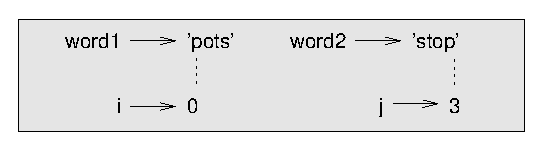
\includegraphics{figs/state4.eps}}
\afterfig

I took a little license by arranging the variables in the frame
and adding dotted lines to show that the values of {\tt i} and
{\tt j} indicate characters in {\tt word1} and {\tt word2}.

\begin{exercise}
\label{is_reverse}
Starting with this diagram, execute the program on paper, changing the
values of {\tt i} and {\tt j} during each iteration.  Find and fix the
second error in this function.
\end{exercise}



\section{Glossary}
	
\begin{vocabulary}[object:] Something a variable can refer to.  For now,
you can use ``object'' and ``value'' interchangeably.
\index{object}
\end{vocabulary}
	
\begin{vocabulary}[sequence:] An ordered set; that is, a set of
values where each value is identified by an integer index.
\index{sequence}
\end{vocabulary}
	
\begin{vocabulary}[item:] One of the values in a sequence.
\index{item}
\end{vocabulary}
	
\begin{vocabulary}[index:] An integer value used to select an item in
a sequence, such as a character in a string.
\index{index}
\end{vocabulary}
	
\begin{vocabulary}[slice:] A part of a string specified by a range of indices.
\index{slice}
\end{vocabulary}
	
\begin{vocabulary}[empty string:] A string with no characters and length 0, represented
by two quotation marks.
\index{empty string}
\end{vocabulary}
	
\begin{vocabulary}[immutable:] The property of a sequence whose items cannot
be assigned.
\index{immutability}
\end{vocabulary}
	
\begin{vocabulary}[traverse:] To iterate through the items in a sequence,
performing a similar operation on each.
\index{traversal}
\end{vocabulary}
	
\begin{vocabulary}[search:] A pattern of traversal that stops
when it finds what it is looking for.
\index{search pattern}
\index{pattern!search}
\end{vocabulary}
	
\begin{vocabulary}[counter:] A variable used to count something, usually initialized
to zero and then incremented.
\index{counter}
\end{vocabulary}
	
\begin{vocabulary}[method:] A function that is associated with an object and called
using dot notation.
\index{method}
\end{vocabulary}
	
\begin{vocabulary}[invocation:] A statement that calls a method.
\index{invocation}
\end{vocabulary}
	


\section{Exercises}

\begin{exercise}

\index{step size}
\index{slice operator}
\index{operator!slice}

A string slice can take a third index that specifies the ``step
size;'' that is, the number of spaces between successive characters.
A step size of 2 means every other character; 3 means every third,
etc.

\beforeverb
\begin{pyexo}
>>> fruit = 'banana'
>>> fruit[0:5:2]
'bnn'
\end{pyexo}
\afterverb

A step size of -1 goes through the word backwards, so
the slice \verb"[::-1]" generates a reversed string.
%
\index{palindrome}
%
Use this idiom to write a one-line version of \verb"is_palindrome"
from Exercise~\ref{palindrome}.
\end{exercise}


\begin{exercise}
\index{string method}
\index{method!string}

Read the documentation of the string methods at
\url{docs.python.org/lib/string-methods.html}.  You
might want to experiment with some of them to make sure
you understand how they work.  {\tt strip} and
{\tt replace} are particularly useful.
%
The documentation uses a syntax that might be confusing.
For example, in \verb"find(sub[, start[, end]])", the brackets
indicate optional arguments.  So {\tt sub} is required, but
{\tt start} is optional, and if you include {\tt start},
then {\tt end} is optional.
\end{exercise}

\begin{exercise}
The following functions are all {\em intended} to check whether a
string contains any lowercase letters, but at least some of them are
wrong.  For each function, describe what the function actually does
(assuming that the parameter is a string).

\begin{pyexo}
def any_lowercase1(s):
    for c in s:
        if c.islower():
            return True
        else:
            return False
\end{pyexo}

\begin{pyexo}
def any_lowercase2(s):
    for c in s:
        if 'c'.islower():
            return 'True'
        else:
            return 'False'
\end{pyexo}

\begin{pyexo}
def any_lowercase3(s):
    for c in s:
        flag = c.islower()
    return flag
\end{pyexo}

\begin{pyexo}
def any_lowercase4(s):
    flag = False
    for c in s:
        flag = flag or c.islower()
    return flag
\end{pyexo}

\begin{pyexo}
def any_lowercase5(s):
    for c in s:
        if not c.islower():
            return False
    return True
\end{pyexo}

\end{exercise}


\begin{exercise}
\index{letter rotation}
\index{rotation, letter}

\label{exrotate}
ROT13 is a weak form of encryption that involves ``rotating'' each
letter in a word by 13 places\footnote{See
  \url{wikipedia.org/wiki/ROT13}.}.  To rotate a letter means
to shift it through the alphabet, wrapping around to the beginning if
necessary, so 'A' shifted by 3 is 'D' and 'Z' shifted by 1 is 'A'.

Write a function called \verb"rotate_word"
that takes a string and an integer as parameters, and that returns
a new string that contains the letters from the original string
``rotated'' by the given amount.  

For example, ``cheer'' rotated by 7 is ``jolly'' and ``melon'' rotated
by -10 is ``cubed''.  
%
%%For example ``sleep''
%%rotated by 9 is ``bunny'' and ``latex'' rotated by 7 is ``shale''.
%
You might want to use the built-in functions {\tt ord}, which converts
a character to a numeric code, and {\tt chr}, which converts numeric
codes to characters.
%
%Potentially offensive jokes on the Internet are sometimes encoded
%in ROT13.  If you are not easily offended, find and decode some
%of them.
\end{exercise}


%\chapterimage{chapter_head_1.pdf}
\chapter{Lists}

\index{list}
\index{type!list}


\section{A list is a sequence}

Like a string, a {\bf list} is a sequence of values.  In a string, the
values are characters; in a list, they can be any type.  The values in
a list are called {\bf elements} or sometimes {\bf items}.

\index{element}
\index{sequence}
\index{item}

There are several ways to create a new list; the simplest is to
enclose the elements in square brackets (\verb"[" and \verb"]"):

\beforeverb
\begin{pyoutput}
[10, 20, 30, 40]
['crunchy frog', 'ram bladder', 'lark vomit']
\end{pyoutput}
\afterverb
%
The first example is a list of four integers.  The second is a list of
three strings.  The elements of a list don't have to be the same type.
The following list contains a string, a float, an integer, and another list:

\beforeverb
\begin{pyoutput}
['spam', 2.0, 5, [10, 20]]
\end{pyoutput}
\afterverb
%
A list within another list is {\bf nested}.
%
\index{nested list}
\index{list!nested}
%
A list that contains no elements is
called an empty list; you can create one with empty
brackets, \verb"[]".
%
\index{empty list}
\index{list!empty}
%
As you might expect, you can assign list values to variables:

\beforeverb
\begin{pycode}
>>> cheeses = ['Cheddar', 'Edam', 'Gouda']
>>> numbers = [17, 123]
>>> empty = []
>>> print(cheeses, numbers, empty)
['Cheddar', 'Edam', 'Gouda'] [17, 123] []
\end{pycode}
\afterverb
%

\index{assignment}

% From Jeff: write sum for a nested list?


\section{Lists are mutable}

\index{list!element}
\index{access}
\index{index}
\index{bracket operator}
\index{operator!bracket}

The syntax for accessing the elements of a list is the same as for
accessing the characters of a string---the bracket operator.  The
expression inside the brackets specifies the index.  Remember that the
indices start at 0:

\beforeverb
\begin{pycode}
>>> print(cheeses[0])
Cheddar
\end{pycode}
\afterverb
%
Unlike strings, lists are mutable.  When the bracket operator appears
on the left side of an assignment, it identifies the element of the
list that will be assigned.

\index{mutability}

\beforeverb
\begin{pycode}
>>> numbers = [17, 123]
>>> numbers[1] = 5
>>> print(numbers)
[17, 5]
\end{pycode}
\afterverb
%
The one-eth element of {\tt numbers}, which
used to be 123, is now 5.

\index{index!starting at zero}
\index{zero, index starting at}

You can think of a list as a relationship between indices and
elements.  This relationship is called a {\bf mapping}; each index
``maps to'' one of the elements.  Here is a state diagram showing {\tt
cheeses}, {\tt numbers} and {\tt empty}:

\index{state diagram}
\index{diagram!state}
\index{mapping}

\beforefig
\centerline{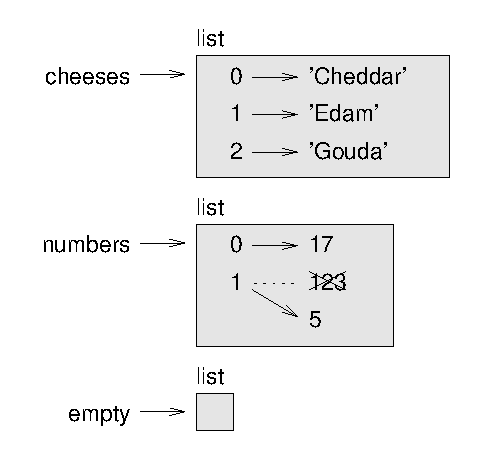
\includegraphics{figs/list_state.eps}}
\afterfig

Lists are represented by boxes with the word ``list'' outside
and the elements of the list inside.  {\tt cheeses} refers to
a list with three elements indexed 0, 1 and 2.
{\tt numbers} contains two elements; the diagram shows that the
value of the second element has been reassigned from 123 to 5.
{\tt empty} refers to a list with no elements.
%
\index{item assignment}
\index{assignment!item}
%
List indices work the same way as string indices:

\begin{itemize}

\item Any integer expression can be used as an index.

\item If you try to read or write an element that does not exist, you
get an {\tt IndexError}.

\index{exception!IndexError}
\index{IndexError}

\item If an index has a negative value, it counts backward from the
end of the list.

\end{itemize}

\index{list!index}


\index{list!membership}
\index{membership!list}
\index{in operator}
\index{operator!in}

The {\tt in} operator also works on lists.

\beforeverb
\begin{pycode}
>>> cheeses = ['Cheddar', 'Edam', 'Gouda']
>>> 'Edam' in cheeses
True
>>> 'Brie' in cheeses
False
\end{pycode}
\afterverb


\section{Traversing a list}
\index{list!traversal}
\index{traversal!list}
\index{for loop}
\index{loop!for}
\index{statement!for}

The most common way to traverse the elements of a list is
with a {\tt for} loop.  The syntax is the same as for strings:

\beforeverb
\begin{pycode}
for cheese in cheeses:
    print(cheese)
\end{pycode}
\afterverb
%
This works well if you only need to read the elements of the
list.  But if you want to write or update the elements, you
need the indices.  A common way to do that is to combine
the functions {\tt range} and {\tt len}:

\index{looping!with indices}
\index{index!looping with}

\beforeverb
\begin{pycode}
for i in range(len(numbers)):
    numbers[i] = numbers[i] * 2
\end{pycode}
\afterverb
%
This loop traverses the list and updates each element.  {\tt len}
returns the number of elements in the list.  {\tt range} returns
a list of indices from 0 to $n-1$, where $n$ is the length of
the list.  Each time through the loop {\tt i} gets the index
of the next element.  The assignment statement in the body uses
{\tt i} to read the old value of the element and to assign the
new value.

\index{item update}
\index{update!item}

A {\tt for} loop over an empty list never executes the body:

\beforeverb
\begin{pycode}
for x in []:
    print('This never happens.')
\end{pycode}
\afterverb
%
Although a list can contain another list, the nested
list still counts as a single element.  The length of this list is
four:

\index{nested list}
\index{list!nested}

\beforeverb
\begin{pyoutput}
['spam', 1, ['Brie', 'Roquefort', 'Pol le Veq'], [1, 2, 3]]
\end{pyoutput}
\afterverb



\section{List operations}
\index{list!operation}

The {\tt +} operator concatenates lists:

\index{concatenation!list}
\index{list!concatenation}

\beforeverb
\begin{pycode}
>>> a = [1, 2, 3]
>>> b = [4, 5, 6]
>>> c = a + b
>>> print(c)
[1, 2, 3, 4, 5, 6]
\end{pycode}
\afterverb
%
Similarly, the {\tt *} operator repeats a list a given number of times:

\index{repetition!list}
\index{list!repetition}

\beforeverb
\begin{pycode}
>>> [0] * 4
[0, 0, 0, 0]
>>> [1, 2, 3] * 3
[1, 2, 3, 1, 2, 3, 1, 2, 3]
\end{pycode}
\afterverb
%
The first example repeats {\tt [0]} four times.  The second example
repeats the list {\tt [1, 2, 3]} three times.


\section{List slices}

\index{slice operator}
\index{operator!slice}
\index{index!slice}
\index{list!slice}
\index{slice!list}

The slice operator also works on lists:

\beforeverb
\begin{pycode}
>>> t = ['a', 'b', 'c', 'd', 'e', 'f']
>>> t[1:3]
['b', 'c']
>>> t[:4]
['a', 'b', 'c', 'd']
>>> t[3:]
['d', 'e', 'f']
\end{pycode}
\afterverb
%
If you omit the first index, the slice starts at the beginning.
If you omit the second, the slice goes to the end.  So if you
omit both, the slice is a copy of the whole list.

\index{list!copy}
\index{slice!copy}
\index{copy!slice}

\beforeverb
\begin{pycode}
>>> t[:]
['a', 'b', 'c', 'd', 'e', 'f']
\end{pycode}
\afterverb
%
Since lists are mutable, it is often useful to make a copy
before performing operations that fold, spindle or mutilate
lists.

\index{mutability}

A slice operator on the left side of an assignment
can update multiple elements:

\index{slice!update}
\index{update!slice}

\beforeverb
\begin{pycode}
>>> t = ['a', 'b', 'c', 'd', 'e', 'f']
>>> t[1:3] = ['x', 'y']
>>> print(t)
['a', 'x', 'y', 'd', 'e', 'f']
\end{pycode}
\afterverb
%

% You can add elements to a list by squeezing them into an empty
% slice:

% \beforeverb
% \begin{pycode}
% >>> t = ['a', 'd', 'e', 'f']
% >>> t[1:1] = ['b', 'c']
% >>> print t
% ['a', 'b', 'c', 'd', 'e', 'f']
% \end{pycode}
% \afterverb
%
% And you can remove elements from a list by assigning the empty list to
% them:

% \beforeverb
% \begin{pycode}
% >>> t = ['a', 'b', 'c', 'd', 'e', 'f']
% >>> t[1:3] = []
% >>> print t
% ['a', 'd', 'e', 'f']
% \end{pycode}
% \afterverb
%
% But both of those operations can be expressed more clearly
% with list methods.


\section{List methods}

\index{list!method}
\index{method, list}

Python provides methods that operate on lists.  For example,
{\tt append} adds a new element to the end of a list:

\index{append method}
\index{method!append}

\beforeverb
\begin{pycode}
>>> t = ['a', 'b', 'c']
>>> t.append('d')
>>> print(t)
['a', 'b', 'c', 'd']
\end{pycode}
\afterverb
%
{\tt extend} takes a list as an argument and appends all of
the elements:

\index{extend method}
\index{method!extend}

\beforeverb
\begin{pycode}
>>> t1 = ['a', 'b', 'c']
>>> t2 = ['d', 'e']
>>> t1.extend(t2)
>>> print(t1)
['a', 'b', 'c', 'd', 'e']
\end{pycode}
\afterverb
%
This example leaves {\tt t2} unmodified.

{\tt sort} arranges the elements of the list from low to high:

\index{sort method}
\index{method!sort}

\beforeverb
\begin{pycode}
>>> t = ['d', 'c', 'e', 'b', 'a']
>>> t.sort()
>>> print(t)
['a', 'b', 'c', 'd', 'e']
\end{pycode}
\afterverb
%
List methods are all void; they modify the list and return {\tt None}.
If you accidentally write {\tt t = t.sort()}, you will be disappointed
with the result.

\index{void method}
\index{method!void}
\index{None special value}
\index{special value!None}


\section{Map, filter and reduce}

To add up all the numbers in a list, you can use a loop like this:

% see add.py

\beforeverb
\begin{pycode}
def add_all(a_list):
    total = 0
    for val in a_list:
        total += val
    return total
\end{pycode}
\afterverb
%
{\tt total} is initialized to 0.  Each time through the loop,
{\tt x} gets one element from the list.  The {\tt +=} operator
provides a short way to update a variable.  This 
{\bf augmented assignment statement}:

\index{update operator}
\index{operator!update}

\index{assignment!augmented}
\index{augmented assignment}

\beforeverb
\begin{pycode}
    total += val
\end{pycode}
\afterverb
%
is equivalent to:

\beforeverb
\begin{pycode}
    total = total + val
\end{pycode}
\afterverb
%
As the loop executes, {\tt total} accumulates the sum of the
elements; a variable used this way is sometimes called an
{\bf accumulator}.
%
\index{accumulator!sum}
%
Adding up the elements of a list is such a common operation
that Python provides it as a built-in function, {\tt sum}:

\beforeverb
\begin{pycode}
>>> t = [1, 2, 3]
>>> sum(t)
6
\end{pycode}
\afterverb
%
An operation like this that combines a sequence of elements into
a single value is sometimes called {\bf reduce}.

\index{reduce pattern}
\index{pattern!reduce}
\index{traversal}

Sometimes you want to traverse one list while building
another.  For example, the following function takes a list of strings
and returns a new list that contains capitalized strings:

\beforeverb
\begin{pycode}
def capitalize_all(word):
    result = []
    for letter in word:
        result.append(letter.capitalize())
    return result
\end{pycode}
\afterverb
%
{\tt result} is initialized with an empty list; each time through
the loop, we append the next element.  So {\tt result} is another
kind of accumulator.
%
\index{accumulator!list}
%
An operation like \verb"capitalize_all" is sometimes called a {\bf
map} because it ``maps'' a function (in this case the method {\tt
capitalize}) onto each of the elements in a sequence.

\index{map pattern}
\index{pattern!map}
\index{filter pattern}
\index{pattern!filter}

Another common operation is to select some of the elements from
a list and return a sublist.  For example, the following
function takes a list of strings and returns a list that contains
only the uppercase strings:

\beforeverb
\begin{pycode}
def only_upper(word):
    result = []
    for letter in word:
        if letter.isupper():
            result.append(letter)
    return result
\end{pycode}
\afterverb
%
{\tt isupper} is a string method that returns {\tt True} if
the string contains only upper case letters.
%
An operation like \verb"only_upper" is called a {\bf filter} because
it selects some of the elements and filters out the others.

Most common list operations can be expressed as a combination
of map, filter and reduce.  Because these operations are
so common, Python provides language features to support them,
including the built-in function {\tt map} and an operator
called a ``list comprehension.''

\index{list!comprehension}

\begin{exercise}
\label{cumulative}
\index{cumulative sum}

Write a function that takes a list of numbers and returns the
cumulative sum; that is, a new list where the $i$th element
is the sum of the first $i+1$ elements from the original list.
For example, the cumulative sum of {\tt [1, 2, 3]} is
{\tt [1, 3, 6]}. 
\end{exercise}


\section{Deleting elements}

\index{element deletion}
\index{deletion, element of list}

There are several ways to delete elements from a list.  If you
know the index of the element you want, you can use
{\tt pop}:

\index{pop method}
\index{method!pop}

\beforeverb
\begin{pycode}
>>> t = ['a', 'b', 'c']
>>> x = t.pop(1)
>>> print(t)
['a', 'c']
>>> print(x)
b
\end{pycode}
\afterverb
%
{\tt pop} modifies the list and returns the element that was removed.
If you don't provide an index, it deletes and returns the
last element.

If you don't need the removed value, you can use the {\tt del}
operator:

\index{del operator}
\index{operator!del}

\beforeverb
\begin{pycode}
>>> t = ['a', 'b', 'c']
>>> del t[1]
>>> print(t)
['a', 'c']
\end{pycode}
\afterverb
%

If you know the element you want to remove (but not the index), you
can use {\tt remove}:

\index{remove method}
\index{method!remove}

\beforeverb
\begin{pycode}
>>> t = ['a', 'b', 'c']
>>> t.remove('b')
>>> print(t)
['a', 'c']
\end{pycode}
\afterverb
%
The return value from {\tt remove} is {\tt None}.

\index{None special value}
\index{special value!None}

To remove more than one element, you can use {\tt del} with
a slice index:

\beforeverb
\begin{pycode}
>>> t = ['a', 'b', 'c', 'd', 'e', 'f']
>>> del t[1:5]
>>> print(t)
['a', 'f']
\end{pycode}
\afterverb
%
As usual, the slice selects all the elements up to, but not
including, the second index.


\section{Lists and strings}

\index{list}
\index{string}
\index{sequence}

A string is a sequence of characters and a list is a sequence
of values, but a list of characters is not the same as a
string.  To convert from a string to a list of characters,
you can use {\tt list}:

\index{list!function}
\index{function!list}

\beforeverb
\begin{pycode}
>>> s = 'spam'
>>> t = list(s)
>>> print(t)
['s', 'p', 'a', 'm']
\end{pycode}
\afterverb
%
Because {\tt list} is the name of a built-in function, you should
avoid using it as a variable name.  I also avoid {\tt l} because
it looks too much like {\tt 1}.  So that's why I use {\tt t}.

The {\tt list} function breaks a string into individual letters.  If
you want to break a string into words, you can use the {\tt split}
method:

\index{split method}
\index{method!split}

\beforeverb
\begin{pycode}
>>> s = 'pining for the fjords'
>>> t = s.split()
>>> print(t)
['pining', 'for', 'the', 'fjords']
\end{pycode}
\afterverb
%
An optional argument called a {\bf delimiter} specifies which
characters to use as word boundaries.
The following example
uses a hyphen as a delimiter:

\index{optional argument}
\index{argument!optional}
\index{delimiter}

\beforeverb
\begin{pycode}
>>> s = 'spam-spam-spam'
>>> delimiter = '-'
>>> s.split(delimiter)
['spam', 'spam', 'spam']
\end{pycode}
\afterverb
%
{\tt join} is the inverse of {\tt split}.  It
takes a list of strings and
concatenates the elements.  {\tt join} is a string method,
so you have to invoke it on the delimiter and pass the
list as a parameter:

\index{join method}
\index{method!join}
\index{concatenation}

\beforeverb
\begin{pycode}
>>> t = ['pining', 'for', 'the', 'fjords']
>>> delimiter = '-'
>>> delimiter.join(t)
'pining-for-the-fjords'
\end{pycode}
\afterverb
%
In this case the delimiter is a space character, so
{\tt join} puts a '-' between words.  To concatenate
strings without delimiters, you can use the empty string,
\verb"''", as a delimiter. 

\index{empty string}
\index{string!empty}


\section{Objects and values}

\index{object}
\index{value}

If we execute these assignment statements:

\beforeverb
\begin{pycode}
a = 'banana'
b = 'banana'
\end{pycode}
\afterverb
%
We know that {\tt a} and {\tt b} both refer to a
string, but we don't
know whether they refer to the {\em same} string.
There are two possible states:

\index{aliasing}

\beforefig
\centerline{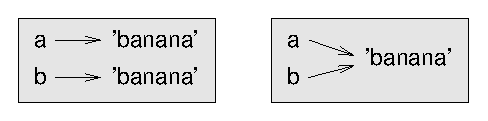
\includegraphics{figs/list1.eps}}
\afterfig

In one case, {\tt a} and {\tt b} refer to two different objects that
have the same value.  In the second case, they refer to the same
object.

\index{is operator}
\index{operator!is}

To check whether two variables refer to the same object, you can
use the {\tt is} operator.

\beforeverb
\begin{pycode}
>>> a = 'banana'
>>> b = 'banana'
>>> a is b
True
\end{pycode}
\afterverb
%
In this example, Python only created one string object,
and both {\tt a} and {\tt b} refer to it.

But when you create two lists, you get two objects:

\beforeverb
\begin{pycode}
>>> a = [1, 2, 3]
>>> b = [1, 2, 3]
>>> a is b
False
\end{pycode}
\afterverb
%
So the state diagram looks like this:

\index{state diagram}
\index{diagram!state}

\beforefig
\centerline{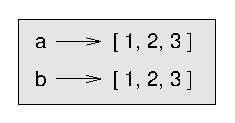
\includegraphics{figs/list2.eps}}
\afterfig

In this case we would say that the two lists are {\bf equivalent},
because they have the same elements, but not {\bf identical}, because
they are not the same object.  If two objects are identical, they are
also equivalent, but if they are equivalent, they are not necessarily
identical.

\index{equivalence}
\index{identity}

Until now, we have been using ``object'' and ``value''
interchangeably, but it is more precise to say that an object has a
value.  If you execute {\tt [1,2,3]}, you get a list
object whose value is a sequence of integers.  If another
list has the same elements, we say it has the same value, but
it is not the same object.

\index{object}
\index{value}


\section{Aliasing}

\index{aliasing}
\index{reference!aliasing}

If {\tt a} refers to an object and you assign {\tt b = a},
then both variables refer to the same object:

\beforeverb
\begin{pycode}
>>> a = [1, 2, 3]
>>> b = a
>>> b is a
True
\end{pycode}
\afterverb
%
The state diagram looks like this:

\index{state diagram}
\index{diagram!state}

\beforefig
\centerline{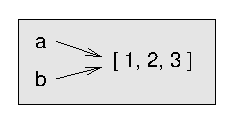
\includegraphics{figs/list3.eps}}
\afterfig

The association of a variable with an object is called a {\bf
reference}.  In this example, there are two references to the same
object.
%
\index{reference}
%
An object with more than one reference has more
than one name, so we say that the object is {\bf aliased}.

\index{mutability}

If the aliased object is mutable, 
changes made with one alias affect
the other:

\beforeverb
\begin{pycode*}{firstnumber = last}
>>> b[0] = 17
>>> print(a)
[17, 2, 3]
\end{pycode*}
\afterverb
%
Although this behavior can be useful, it is error-prone.  In general,
it is safer to avoid aliasing when you are working with mutable
objects.

\index{immutability}

For immutable objects like strings, aliasing is not as much of a
problem.  In this example:

\beforeverb
\begin{pycode}
a = 'banana'
b = 'banana'
\end{pycode}
\afterverb
%
It almost never makes a difference whether {\tt a} and {\tt b} refer
to the same string or not.


\section{List arguments}

\index{list!as argument}
\index{argument}
\index{argument!list}
\index{reference}
\index{parameter}

When you pass a list to a function, the function gets a reference
to the list.
If the function modifies a list parameter, the caller sees the change.
For example, \verb"delete_head" removes the first element from a list:

\beforeverb
\begin{pycode}
def delete_head(lst):
    del lst[0]
\end{pycode}
\afterverb
%
Here's how it is used:

\beforeverb
\begin{pycode}
>>> letters = ['a', 'b', 'c']
>>> delete_head(letters)
>>> print (letters)
['b', 'c']
\end{pycode}
\afterverb
%
The parameter {\tt lst} and the variable {\tt letters} are
aliases for the same object.  The stack diagram looks like
this:

\index{stack diagram}
\index{diagram!stack}

\beforefig
\centerline{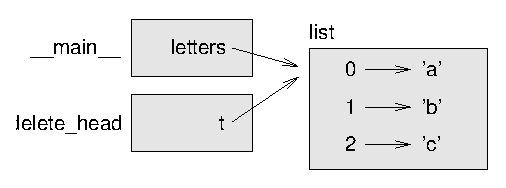
\includegraphics{figs/stack5.eps}}
\afterfig

Since the list is shared by two frames, I drew
it between them.

It is important to distinguish between operations that
modify lists and operations that create new lists.  For
example, the {\tt append} method modifies a list, but the
{\tt +} operator creates a new list:

\index{append method}
\index{method!append}
\index{list!concatenation}
\index{concatenation!list}

\beforeverb
\begin{pycode}
>>> t1 = [1, 2]
>>> t2 = t1.append(3)
>>> print(t1)
[1, 2, 3]
>>> print(t2)
None

>>> t1 = [1, 2]
>>> t3 = t1 + [3]
>>> print (t3)
[1, 2, 3]
>>> t2 is t3
False
\end{pycode}
\afterverb

This difference is important when you write functions that
are supposed to modify lists.  For example, this function
{\em does not} delete the head of a list:

\beforeverb
\begin{pycode}
def bad_delete_head(t):
    t = t[1:]              # WRONG!
\end{pycode}
\afterverb

The slice operator creates a new list and the assignment
makes {\tt t} refer to it, but none of that has any effect
on the list that was passed as an argument.{\color{red} MUST EXPAND ON THIS}

\index{slice operator}
\index{operator!slice}

An alternative is to write a function that creates and
returns a new list.  For
example, {\tt tail} returns all but the first
element of a list:

\beforeverb
\begin{pycode}
def tail(t):
    return t[1:]
\end{pycode}
\afterverb
%
This function leaves the original list unmodified.
Here's how it is used:

\beforeverb
\begin{pycode}
>>> letters = ['a', 'b', 'c']
>>> rest = tail(letters)
>>> print(rest)
['b', 'c']
\end{pycode}
\afterverb


\begin{exercise}

Write a function called {\tt chop} that takes a list and modifies
it, removing the first and last elements, and returns {\tt None}.

Then write a function called {\tt middle} that takes a list and
returns a new list that contains all but the first and last
elements.

\end{exercise}


\section{Debugging}
\index{debugging}

Careless use of lists (and other mutable objects)
can lead to long hours of debugging.  Here are some common
pitfalls and ways to avoid them:

\begin{enumerate}

\item Don't forget that most list methods modify the argument and
  return {\tt None}.  This is the opposite of the string methods,
  which return a new string and leave the original alone.

If you are used to writing string code like this:

\beforeverb
\begin{pycode}
word = word.strip()
\end{pycode}
\afterverb

It is tempting to write list code like this:

\beforeverb
\begin{pycode}
t = t.sort()           # WRONG!
\end{pycode}
\afterverb

\index{sort method}
\index{method!sort}

Because {\tt sort} returns {\tt None}, the
next operation you perform with {\tt t} is likely to fail.

Before using list methods and operators, you should read the
documentation carefully and then test them in interactive mode.  The
methods and operators that lists share with other sequences (like
strings) are documented at
\url{docs.python.org/lib/typesseq.html}.  The
methods and operators that only apply to mutable sequences
are documented at \url{docs.python.org/lib/typesseq-mutable.html}.


\item Pick an idiom and stick with it.

Part of the problem with lists is that there are too many
ways to do things.  For example, to remove an element from
a list, you can use {\tt pop}, {\tt remove}, {\tt del},
or even a slice assignment.
%
To add an element, you can use the {\tt append} method or
the {\tt +} operator.  Assuming that {\tt t} is a list and
{\tt x} is a list element, these are right: 

\beforeverb
\begin{pycode}
t.append(x)
t = t + [x]
\end{pycode}
\afterverb

And these are wrong:

\beforeverb
\begin{pycode}
t.append([x])          # WRONG!
t = t.append(x)        # WRONG!
t + [x]                # WRONG!
t = t + x              # WRONG!
\end{pycode}
\afterverb

Try out each of these examples in interactive mode to make sure
you understand what they do.  Notice that only the last
one causes a runtime error; the other three are legal, but they
do the wrong thing.


\item Make copies to avoid aliasing.

\index{aliasing!copying to avoid}
\index{copy!to avoid aliasing}

If you want to use a method like {\tt sort} that modifies
the argument, but you need to keep the original list as
well, you can make a copy.

\beforeverb
\begin{pycode}
orig = t[:]
t.sort()
\end{pycode}
\afterverb

In this example you could also use the built-in function {\tt sorted},
which returns a new, sorted list and leaves the original alone.
But in that case you should avoid using {\tt sorted} as a variable
name!

\end{enumerate}



\section{Glossary}
	
\begin{vocabulary}[list:] A sequence of values.
\index{list}
\end{vocabulary}
	
\begin{vocabulary}[element:] One of the values in a list (or other sequence),
also called items.
\index{element}
\end{vocabulary}
	
\begin{vocabulary}[index:] An integer value that indicates an element in a list.
\index{index}
\end{vocabulary}
	
\begin{vocabulary}[nested list:] A list that is an element of another list.
\index{nested list}
\end{vocabulary}
	
\begin{vocabulary}[list traversal:] The sequential accessing of each element in a list.
\index{list!traversal}
\end{vocabulary}
	
\begin{vocabulary}[mapping:] A relationship in which each element of one set
corresponds to an element of another set.  For example, a list is
a mapping from indices to elements.
\index{mapping}
\end{vocabulary}
	
\begin{vocabulary}[accumulator:] A variable used in a loop to add up or
accumulate a result.
\index{accumulator}
\end{vocabulary}
	
\begin{vocabulary}[augmented assignment:] A statement that updates the value
of a variable using an operator like \verb"+=".
\index{assignment!augmented}
\index{augmented assignment}
\index{traversal}
\end{vocabulary}
	
\begin{vocabulary}[reduce:] A processing pattern that traverses a sequence 
and accumulates the elements into a single result.
\index{reduce pattern}
\index{pattern!reduce}
\end{vocabulary}
	
\begin{vocabulary}[map:] A processing pattern that traverses a sequence and
performs an operation on each element.
\index{map pattern}
\index{pattern!map}
\end{vocabulary}
	
\begin{vocabulary}[filter:] A processing pattern that traverses a list and
selects the elements that satisfy some criterion.
\index{filter pattern}
\index{pattern!filter}
\end{vocabulary}
	
\begin{vocabulary}[object:] Something a variable can refer to.  An object
has a type and a value.
\index{object}
\end{vocabulary}
	
\begin{vocabulary}[equivalent:] Having the same value.
\index{equivalent}
\end{vocabulary}
	
\begin{vocabulary}[identical:] Being the same object (which implies equivalence).
\index{identical}
\end{vocabulary}
	
\begin{vocabulary}[reference:] The association between a variable and its value.
\index{reference}
\end{vocabulary}
	
\begin{vocabulary}[aliasing:] A circumstance where two or more variables refer to the same
object.
\index{aliasing}
\end{vocabulary}
	
\begin{vocabulary}[delimiter:] A character or string used to indicate where a
string should be split.
\index{delimiter}
\end{vocabulary}
	


\section{Exercises}

\begin{exercise}
Write a function called \verb"is_sorted" that takes a list as a
parameter and returns {\tt True} if the list is sorted in ascending
order and {\tt False} otherwise.  You can assume (as a precondition)
that the elements of the list can be compared with the relational
operators {\tt <}, {\tt >}, etc.

\index{precondition}

For example, \verb"is_sorted([1,2,2])" should return {\tt True}
and \verb"is_sorted(['b','a'])" should return {\tt False}.
\end{exercise}


\begin{exercise}
\label{anagram}

\index{anagram}

Two words are anagrams if you can rearrange the letters from one
to spell the other.  Write a function called \verb"is_anagram"
that takes two strings and returns {\tt True} if they are anagrams.
\end{exercise}


\begin{exercise}
\label{duplicate}

The (so-called) Birthday Paradox:

\begin{enumerate}

\index{birthday paradox}
\index{duplicate}

\item Write a function called \verb"has_duplicates" that takes
a list and returns {\tt True} if there is any element that
appears more than once.  It should not modify the original
list.

\item If there are 23 students in your class, what are the chances
that two of you have the same birthday?  You can estimate this
probability by generating random samples of 23 birthdays
and checking for matches.  Hint: you can generate random birthdays
with the {\tt randint} function in the {\tt random} module.

\index{random module}
\index{module!random}
\index{randint function}
\index{function!randint}

\end{enumerate}

You can read about this problem at
\url{wikipedia.org/wiki/Birthday_paradox}, and you can see my solution
at \url{thinkpython.com/code/birthday.py}.

\end{exercise}


\begin{exercise}

\index{duplicate}
\index{uniqueness}

Write a function called \verb"remove_duplicates" that takes
a list and returns a new list with only the unique elements from
the original.  Hint: they don't have to be in the same order.
\end{exercise}


\begin{exercise}
\index{append method}
\index{method append}
\index{list!concatenation}
\index{concatenation!list}

Write a function that reads the file {\tt words.txt} and builds
a list with one element per word.  Write two versions of
this function, one using the {\tt append} method and the
other using the idiom {\tt t = t + [x]}.  Which one takes
longer to run?  Why?

You can see my solution at \url{thinkpython.com/code/wordlist.py}.
\end{exercise}


\begin{exercise}
\label{wordlist1}
\label{bisection}

\index{membership!bisection search}
\index{bisection search}
\index{search, bisection}

\index{membership!binary search}
\index{binary search}
\index{search, binary}

To check whether a word is in the word list, you could use
the {\tt in} operator, but it would be slow because it searches
through the words in order.

Because the words are in alphabetical order, we can speed things up
with a bisection search (also known as binary search), which is
similar to what you do when you look a word up in the dictionary.  You
start in the middle and check to see whether the word you are looking
for comes before the word in the middle of the list.  If so, then you
search the first half of the list the same way.  Otherwise you search
the second half.

Either way, you cut the remaining search space in half.  If the
word list has 113,809 words, it will take about 17 steps to
find the word or conclude that it's not there.

Write a function called {\tt bisect} that takes a sorted list
and a target value and returns the index of the value
in the list, if it's there, or {\tt None} if it's not.

\index{bisect module}
\index{module!bisect}

Or you could read the documentation of the {\tt bisect} module
and use that!
\end{exercise}

\begin{exercise}
\index{reverse word pair}

Two words are a ``reverse pair'' if each is the reverse of the
other.  Write a program that finds all the reverse pairs in the
word list. 
\end{exercise}

\begin{exercise}
\index{interlocking words}

Two words ``interlock'' if taking alternating letters from each forms
a new word\footnote{This exercise is inspired by an example at
  \url{puzzlers.org}.}.  For example, ``shoe'' and ``cold''
interlock to form ``schooled.''

\begin{enumerate}

\item Write a program that finds all pairs of words that interlock.
  Hint: don't enumerate all pairs!

\item Can you find any words that are three-way interlocked; that is,
  every third letter forms a word, starting from the first, second or
  third?

\end{enumerate}
\end{exercise}




%\chapterimage{chapter_head_1.pdf}
\chapter{Dictionaries}
\index{dictionary}

\index{type!dict}
\index{key}
\index{key-value pair}
\index{index}

A {\bf dictionary} is like a list, but more general.  In a list,
the indices have to be integers; in a dictionary they can
be (almost) any type.

You can think of a dictionary as a mapping between a set of indices
(which are called {\bf keys}) and a set of values.  Each key maps to a
value.  The association of a key and a value is called a {\bf
  key-value pair} or sometimes an {\bf item}.

As an example, we'll build a dictionary that maps from English
to French words, so the keys and the values are all strings.

The function {\tt dict} creates a new dictionary with no items.
Because {\tt dict} is the name of a built-in function, you
should avoid using it as a variable name.

\index{dict function}
\index{function!dict}

\beforeverb
\begin{pyinterpreter}
>>> eng2fr = dict()
>>> print(eng2fr)
{}
\end{pyinterpreter}
\afterverb

The curly-brackets, \verb"{}", represent an empty dictionary.
To add items to the dictionary, you can use square brackets:

\index{curly bracket}
\index{bracket!curly}

\beforeverb
\begin{pyinterpreter}
>>> eng2fr['one'] = 'un'
\end{pyinterpreter}
\afterverb
%
This line creates an item that maps from the key
\verb"'one'" to the value \verb"'un'".  If we print the
dictionary again, we see a key-value pair with a colon
between the key and value:

\beforeverb
\begin{pyinterpreter}
>>> print(eng2fr)
{'one': 'un'}
\end{pyinterpreter}
\afterverb
%
This output format is also an input format.  For example,
you can create a new dictionary with three items:

\beforeverb
\begin{pyinterpreter}
>>> eng2fr = {'one': 'un', 'two': 'deux', 'three': 'trois'}
\end{pyinterpreter}
\afterverb
%
But if you print {\tt eng2fr}, you might be surprised:

\beforeverb
\begin{pyinterpreter}
>>> print(eng2fr)
{'one': 'un', 'three': 'trois', 'two': 'deux'}
\end{pyinterpreter}
\afterverb
%
The order of the key-value pairs is not the same.  In fact, if
you type the same example on your computer, you might get a
different result.  In general, the order of items in
a dictionary is unpredictable.
But that's not a problem because
the elements of a dictionary are never indexed with integer indices.
Instead, you use the keys to look up the corresponding values:

\beforeverb
\begin{pyinterpreter}
>>> print(eng2fr['two'])
'deux'
\end{pyinterpreter}
\afterverb
%
The key \verb"'two'" always maps to the value \verb"'deux'" so the order
of the items doesn't matter.
If the key isn't in the dictionary, you get an exception:

\index{exception!KeyError}
\index{KeyError}

\beforeverb
\begin{pyinterpreter}
>>> print(eng2fr['four'])
Traceback (most recent call last):
  File "<pyshell#19>", line 1, in <module>
    print(eng2fr['four'])
KeyError: 'four'
\end{pyinterpreter}
\afterverb
%
The {\tt len} function works on dictionaries; it returns the
number of key-value pairs:

\index{len function}
\index{function!len}

\beforeverb
\begin{pyinterpreter}
>>> len(eng2fr)
3
\end{pyinterpreter}
\afterverb
%
The {\tt in} operator works on dictionaries; it tells you whether
something appears as a {\em key} in the dictionary (appearing
as a value is not good enough).

\index{membership!dictionary}
\index{in operator}
\index{operator!in}

\beforeverb
\begin{pyinterpreter}
>>> 'one' in eng2fr
True
>>> 'un' in eng2fr
False
\end{pyinterpreter}
\afterverb
%
To see whether something appears as a value in a dictionary, you
can use the method {\tt values}, which returns the values as
a list, and then use the {\tt in} operator:

\index{values method}
\index{method!values}

\beforeverb
\begin{pyinterpreter}
>>> vals = eng2fr.values()
>>> 'un' in vals
True
\end{pyinterpreter}
\afterverb
%
The {\tt in} operator uses different algorithms for lists and
dictionaries.  For lists, it uses a search algorithm, as in {\color{red}
Section~\ref{find}}.  As the list gets longer, the search time gets
longer in direct proportion.  For dictionaries, Python uses an
algorithm called a {\bf hashtable} that has a remarkable property: the
{\tt in} operator takes about the same amount of time no matter how
many items there are in a dictionary.  I won't explain how that's
possible, but you can read more about it at
\url{wikipedia.org/wiki/Hash_table}.

\index{hashtable}

\begin{exercise}
\label{wordlist2}

\index{set membership}
\index{membership!set}

Write a function that reads the words in {\tt words.txt} and
stores them as keys in a dictionary.  It doesn't matter what the
values are.  Then you can use the {\tt in} operator
as a fast way to check whether a string is in
the dictionary.

If you did {\color{red} Exercise~\ref{wordlist1}}, you can compare the speed
of this implementation with the list {\tt in} operator and the
bisection search.

\end{exercise}


\section{Dictionary as a set of counters}
\label{histogram}

\index{counter}

Suppose you are given a string and you want to count how many
times each letter appears.  There are several ways you could do it:

\begin{enumerate}

\item You could create 26 variables, one for each letter of the
alphabet.  Then you could traverse the string and, for each
character, increment the corresponding counter, probably using
a chained conditional.

\item You could create a list with 26 elements.  Then you could
convert each character to a number (using the built-in function
{\tt ord}), use the number as an index into the list, and increment
the appropriate counter.

\item You could create a dictionary with characters as keys
and counters as the corresponding values.  The first time you
see a character, you would add an item to the dictionary.  After
that you would increment the value of an existing item.

\end{enumerate}

Each of these options performs the same computation, but each
of them implements that computation in a different way.
%
\index{implementation}
%
An {\bf implementation} is a way of performing a computation;
some implementations are better than others.  For example,
an advantage of the dictionary implementation is that we don't
have to know ahead of time which letters appear in the string
and we only have to make room for the letters that do appear.
%
Here is what the code might look like:

\beforeverb
\begin{pycode}
def histogram(text):
    hist = dict()
    for character in text:
        if character not in hist:
            hist[character] = 1
        else:
            hist[character] += 1
    return hist
\end{pycode}
\afterverb
%
The name of the function is {\bf histogram}, which is a statistical
term for a set of counters (or frequencies).

\index{histogram}
\index{frequency}
\index{traversal}

The first line of the
function creates an empty dictionary named {\tt hist}.  The {\tt for} loop traverses
the string {\tt text}.  Each time through the loop, if the character {\tt character} is
not in the dictionary, we create a new item with key {\tt character} and the
initial value 1 (since we have seen this letter once).  If {\tt character} is
already in the dictionary we increment {\tt hist[character]}.
%
\index{histogram}
%
Here's how it works:

\beforeverb
\begin{pyinterpreter}
>>> h = histogram('brontosaurus')
>>> print(h)
{'a': 1, 'b': 1, 'o': 2, 'n': 1, 's': 2, 'r': 2, 'u': 2, 't': 1}
\end{pyinterpreter}
\afterverb
%
The histogram indicates that the letters \verb"'a'" and \verb"'b'"
appear once; \verb"'o'" appears twice, and so on.

\begin{exercise}

\index{get method}
\index{method!get}

Dictionaries have a method called {\tt get} that takes a key
and a default value.  If the key appears in the dictionary,
{\tt get} returns the corresponding value; otherwise it returns
the default value.  For example:

\beforeverb
\begin{pyexo}
>>> h = histogram('brontosaurus')
>>> print(h)
{'a': 1, 'b': 1, 'o': 2, 'n': 1, 's': 2, 'r': 2, 'u': 2, 't': 1}
>>> h.get('a', 0)
1
>>> h.get('z', 0)
0
\end{pyexo}
\afterverb
%
Use {\tt get} to write {\tt histogram} more concisely.  You
should be able to eliminate the {\tt if} statement.
\end{exercise}


\section{Looping and dictionaries}

\index{dictionary!looping with}
\index{looping!with dictionaries}
\index{traversal}

If you use a dictionary in a {\tt for} statement, it traverses
the keys of the dictionary.  For example, \verb"print_histogram"
prints each key and the corresponding value:

\beforeverb
\begin{pycode}
def print_histogram(hist):
    for character in hist:
        print(character, hist[character])
\end{pycode}
\afterverb
%
Here's what the output looks like:

\beforeverb
\begin{pyinterpreter}
>>> h = histogram('parrot')
>>> print_histogram(h)
a 1
p 1
r 2
t 1
o 1
\end{pyinterpreter}
\afterverb
%
Again, the keys are in no particular order.

\begin{exercise}

\index{keys method}
\index{method!keys}

Dictionaries have a method called {\tt keys} that returns
the keys of the dictionary, in no particular order, as a list.
%
Modify \verb"print_histogram" to print the keys and their values
in alphabetical order.
\end{exercise}



\section{Reverse lookup}

\index{dictionary!lookup}
\index{dictionary!reverse lookup}
\index{lookup, dictionary}
\index{reverse lookup, dictionary}

Given a dictionary {\tt d} and a key {\tt k}, it is easy to
find the corresponding value {\tt v = d[k]}.  This operation
is called a {\bf lookup}.

But what if you have {\tt v} and you want to find {\tt k}?
You have two problems: first, there might be more than one
key that maps to the value {\tt v}.  Depending on the application,
you might be able to pick one, or you might have to make
a list that contains all of them.  Second, there is no
simple syntax to do a {\bf reverse lookup}; you have to search.
%
Here is a function that takes a value and returns the first
key that maps to that value:

\beforeverb
\begin{pycode}
def reverse_lookup(dico, value):
    for key in dico:
        if dico[key] == value:
            return key
    raise ValueError('No such value in dictionary!')
\end{pycode}
\afterverb
%
This function is yet another example of the search pattern, but it
uses a feature we haven't seen before, {\tt raise}.  The {\tt raise}
statement causes an exception; in this case it causes a {\tt
  ValueError}, which generally indicates that there is something wrong
with the value of a parameter.
%
\index{search}
\index{pattern!search}
\index{raise statement}
\index{statement!raise}
\index{exception!ValueError}
\index{ValueError}
%
If we get to the end of the loop, that means {\tt value}
doesn't appear in the dictionary as a value, so we raise an
exception.
%
Here is an example of a successful reverse lookup:

\beforeverb
\begin{pyinterpreter}
>>> h = histogram('brontosaurus')
>>> k = reverse_lookup(h, 1)
>>> print(k)
b
\end{pyinterpreter}
\afterverb
%
And an unsuccessful one:

\beforeverb
\begin{pyinterpreter}
>>> h = histogram('brontosaurus')
>>> k = reverse_lookup(h, 3)
Traceback (most recent call last):
  File "<pyshell#9>", line 1, in <module>
    k = reverse_lookup(h, 3)
  File "D:/Python/dictionaries.py", line 20, in reverse_lookup
    raise ValueError('No such value in dictionary!')
ValueError: No such value in dictionary!
\end{pyinterpreter}
\afterverb
%
The result when you raise an exception is the same as when
Python raises one: it prints a traceback and an error message.
%
\index{traceback}
\index{optional argument}
\index{argument!optional}
%
%The {\tt raise} statement takes a detailed error message as an
%optional argument.  For example:
%
%\beforeverb
%\begin{pycode}
%>>> raise ValueError('value does not appear in the dictionary')
%Traceback (most recent call last):
  %File "<stdin>", line 1, in ?
%ValueError: value does not appear in the dictionary
%\end{pycode}
%\afterverb

A reverse lookup is much slower than a forward lookup; if you
have to do it often, or if the dictionary gets big, the performance
of your program will suffer.

\begin{exercise}
Modify \verb"reverse_lookup" so that it builds and returns a list
of {\em all} keys that map to a value {\tt v}, or an empty list if there
are none.
\end{exercise}


\section{Dictionaries and lists}

Lists can appear as values in a dictionary.  For example, if you
were given a dictionary that maps from letters to frequencies, you
might want to invert it; that is, create a dictionary that maps
from frequencies to letters.  Since there might be several letters
with the same frequency, each value in the inverted dictionary
should be a list of letters.

\index{invert dictionary}
\index{dictionary!invert}

Here is a function that inverts a dictionary:

\beforeverb
\begin{pycode}
def invert_dict(dico):
    inverted = dict()
    for key in dico:
        value = dico[key]
        if value not in inverted:
            inverted[value] = [key]
        else:
            inverted[value].append(key)
    return inverted
\end{pycode}
\afterverb
%
Each time through the loop, {\tt key} gets a key from {\tt dico} and 
{\tt value} gets the corresponding value.  If {\tt value} is not in {\tt inverted},
that means we haven't seen it before, so we create a new item and
initialize it with a {\bf singleton} (a list that contains a
single element).  Otherwise we have seen this value before, so we
append the corresponding key to the list.

\index{singleton}

Here is an example:

\beforeverb
\begin{pyinterpreter}
>>> h = histogram('parrot')
>>> print(h)
{'p': 1, 'a': 1, 'r': 2, 'o': 1, 't': 1}
>>> inv = invert_dict(h)
>>> print(inv)
{1: ['p', 'a', 'o', 't'], 2: ['r']}
\end{pyinterpreter}
\afterverb
%
%And here is a diagram showing {\tt h} and {\tt inv}:
%
%\index{state diagram}
%\index{diagram!state}
%%
%\beforefig
%\centerline{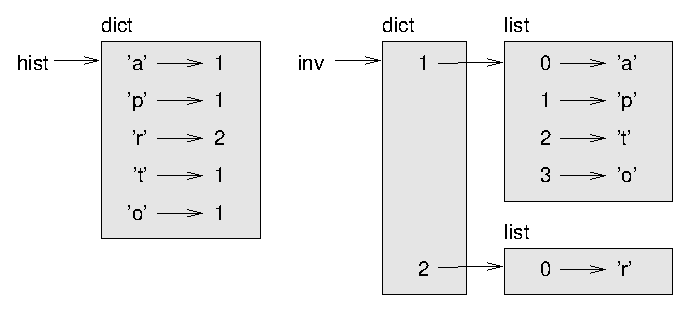
\includegraphics{figs/dict1.eps}}
%\afterfig
%%
%A dictionary is represented as a box with the type {\tt dict} above it
%and the key-value pairs inside.  If the values are integers, floats or
%strings, I usually draw them inside the box, but I usually draw lists
%outside the box, just to keep the diagram simple.

Lists can be values in a dictionary, as this example shows, but they
cannot be keys.  Here's what happens if you try:
%
\index{TypeError}
\index{exception!TypeError}
%

\beforeverb
\begin{pyinterpreter}
>>> lst = [1,2,3]
>>> dico = dict()
>>> dico[lst] = 'oops'
Traceback (most recent call last):
  File "<pyshell#17>", line 1, in <module>
    dico[lst] = 'oops'
TypeError: unhashable type: 'list'
\end{pyinterpreter}
\afterverb
%
I mentioned earlier that a dictionary is implemented using
a hashtable and that means that the keys have to be {\bf hashable}.
%
\index{hash function}
\index{hashable}
%
A {\bf hash} is a function that takes a value (of any kind)
and returns an integer.  Dictionaries use these integers,
called hash values, to store and look up key-value pairs.
%
\index{immutability}
%
This system works fine if the keys are immutable.  But if the
keys are mutable, like lists, bad things happen.  For example,
when you create a key-value pair, Python hashes the key and 
stores it in the corresponding location.  If you modify the
key and then hash it again, it would go to a different location.
In that case you might have two entries for the same key,
or you might not be able to find a key.  Either way, the
dictionary wouldn't work correctly.
%
That's why the keys have to be hashable, and why mutable types like
lists aren't.  {\color{red} The simplest way to get around this limitation is to
use tuples, which we will see in the next chapter.}
%
Since dictionaries are mutable, they can't be used as keys,
but they {\em can} be used as values.

\begin{exercise}
Read the documentation of the dictionary method {\tt setdefault}
and use it to write a more concise version of \verb"invert_dict".

\index{setdefault method}
\index{method!setdefault}

\end{exercise}


\section{Debugging}
\index{debugging}

As you work with bigger datasets it can become unwieldy to
debug by printing and checking data by hand.  Here are some
suggestions for debugging large datasets:

\begin{description}

\item[Scale down the input:] If possible, reduce the size of the
dataset.  For example if the program reads a text file, start with
just the first 10 lines, or with the smallest example you can find.
You can either edit the files themselves, or (better) modify the
program so it reads only the first {\tt n} lines.
%
If there is an error, you can reduce {\tt n} to the smallest
value that manifests the error, and then increase it gradually
as you find and correct errors.

\item[Check summaries and types:] Instead of printing and checking the
entire dataset, consider printing summaries of the data: for example,
the number of items in a dictionary or the total of a list of numbers.
%
A common cause of runtime errors is a value that is not the right
type.  For debugging this kind of error, it is often enough to print
the type of a value.

\item[Write self-checks:]  Sometimes you can write code to check
for errors automatically.  For example, if you are computing the
average of a list of numbers, you could check that the result is
not greater than the largest element in the list or less than
the smallest.  This is called a ``sanity check'' because it detects
results that are ``insane.''
%
\index{sanity check}
\index{consistency check}
%
Another kind of check compares the results of two different
computations to see if they are consistent.  This is called a
``consistency check.''

\item[Pretty print the output:] {\color{red} Formatting debugging output
can make it easier to spot an error.  We saw an example in
Section~\ref{factdebug}.  The {\tt pprint} module provides
a {\tt pprint} function that displays built-in types in
a more human-readable format.}

\index{pretty print}
\index{pprint module}
\index{module!pprint}

\end{description}

Again, time you spend building scaffolding can reduce
the time you spend debugging.

\index{scaffolding}

\section{Glossary}
	
\begin{vocabulary}[dictionary:] A mapping from a set of keys to their
corresponding values.
\index{dictionary}
\end{vocabulary}
	
\begin{vocabulary}[key-value pair:] The representation of the mapping from
a key to a value.
\index{key-value pair}
\end{vocabulary}
	
\begin{vocabulary}[item:] Another name for a key-value pair.
\index{item!dictionary}
\end{vocabulary}
	
\begin{vocabulary}[key:] An object that appears in a dictionary as the
first part of a key-value pair.
\index{key}
\end{vocabulary}
	
\begin{vocabulary}[value:] An object that appears in a dictionary as the
second part of a key-value pair.  This is more specific than
our previous use of the word ``value.''
\index{value}
\end{vocabulary}
	
\begin{vocabulary}[implementation:] A way of performing a computation.
\index{implementation}
\end{vocabulary}
	
\begin{vocabulary}[hashtable:] The algorithm used to implement Python
dictionaries.
\index{hashtable}
\end{vocabulary}
	
\begin{vocabulary}[hash function:] A function used by a hashtable to compute the
location for a key.{\color{red} may want to expend}
\index{hash function}
\end{vocabulary}
	
\begin{vocabulary}[hashable:] A type that has a hash function.  Immutable
types like integers,
floats and strings are hashable; mutable types like lists and
dictionaries are not.
\index{hashable}
\end{vocabulary}
	
\begin{vocabulary}[lookup:] A dictionary operation that takes a key and finds
the corresponding value.
\index{lookup}
\end{vocabulary}
	
\begin{vocabulary}[reverse lookup:] A dictionary operation that takes a value and finds
one or more keys that map to it.
\index{reverse lookup, dictionary}
\end{vocabulary}
	
\begin{vocabulary}[singleton:] A list (or other sequence) with a single element.
\index{singleton}
\end{vocabulary}
	
\begin{vocabulary}[call graph:] A diagram that shows every frame created during
the execution of a program, with an arrow from each caller to
each callee. {\color{red}may want to remove}
\index{call graph}
\index{diagram!call graph}
\end{vocabulary}
	
\begin{vocabulary}[histogram:] A set of counters. {\color{red}find a better definition.}
\index{histogram}
\end{vocabulary}
	
\begin{vocabulary}[memo:] A computed value stored to avoid unnecessary future 
computation.
\index{memo}
\end{vocabulary}
	
\begin{vocabulary}[global variable:]  A variable defined outside a function.  Global
variables can be accessed from any function.
\index{global variable}
\end{vocabulary}
	
\begin{vocabulary}[flag:] A boolean variable used to indicate whether a condition
is true.
\index{flag}
\end{vocabulary}
	
\begin{vocabulary}[declaration:] A statement like {\tt global} that tells the
interpreter something about a variable.
\index{declaration}
\end{vocabulary}
	

\section{Exercises}

\begin{exercise}
\index{duplicate}

If you did {\color{red} Exercise~\ref{duplicate}}, you already have
a function named \verb"has_duplicates" that takes a list
as a parameter and returns {\tt True} if there is any object
that appears more than once in the list.

Use a dictionary to write a faster, simpler version of
\verb"has_duplicates".
\end{exercise}


\begin{exercise}
\label{exrotatepairs}

\index{letter rotation}
\index{rotation!letters}

Two words are ``rotate pairs'' if you can rotate one of them
and get the other {\color{red} (see \verb"rotate_word" in Exercise~\ref{exrotate})}.

Write a program that reads a wordlist and finds all the rotate
pairs.
\end{exercise}


\begin{exercise}
\index{Car Talk}
\index{Puzzler}

Here's another Puzzler from {\em Car
Talk}\footnote{\url{www.cartalk.com/content/puzzler/transcripts/200717}.}:

\begin{quote}
This was sent in by a fellow named Dan O'Leary. He came upon a common
one-syllable, five-letter word recently that has the following unique
property. When you remove the first letter, the remaining letters form
a homophone of the original word, that is a word that sounds exactly
the same. Replace the first letter, that is, put it back and remove
the second letter and the result is yet another homophone of the
original word. And the question is, what's the word?

Now I'm going to give you an example that doesn't work. Let's look at
the five-letter word, `wrack'. W-R-A-C-K, you know like to `wrack with
pain'. If I remove the first letter, I am left with a four-letter
word, R-A-C-K. As in, `Holy cow, did you see the rack on that buck!
It must have been a nine-pointer!' It's a perfect homophone. If you
put the `w' back, and remove the `r', instead, you're left with the
word, `wack', which is a real word, it's just not a homophone of the
other two words.

But there is, however, at least one word that Dan and we know of,
which will yield two homophones if you remove either of the first two
letters to make two, new four-letter words. The question is, what's
the word?
\end{quote}

\index{homophone}
\index{reducible word}
\index{word, reducible}

You can use the dictionary from {\color{red} Exercise~\ref{wordlist2}} to check
whether a string is in the word list.

To check whether two words are homophones, you can use the CMU
Pronouncing Dictionary.  You can download it from
\url{www.speech.cs.cmu.edu/cgi-bin/cmudict} or from
\url{thinkpython.com/code/c06d} and you can also download
\url{thinkpython.com/code/pronounce.py}, which provides a function
named \verb"read_dictionary" that reads the pronouncing dictionary and
returns a Python dictionary that maps from each word to a string that
describes its primary pronunciation.

Write a program that lists all the words that solve the Puzzler.
You can see my solution at \url{thinkpython.com/code/homophone.py}.

\end{exercise}



%\chapterimage{chapter_head_1.pdf}
\chapter{Tuples}
\label{tuplechap}

\section{Tuples are immutable}

\index{tuple}
\index{type!tuple}
\index{sequence}

A tuple is a sequence of values.  The values can be any type, and
they are indexed by integers, so in that respect tuples are a lot
like lists.  The important difference is that tuples are immutable.
%
\index{mutability}
\index{immutability}
%
Syntactically, a tuple is a comma-separated list of values:

\beforeverb
\begin{pycode}
>>> t = 'a', 'b', 'c', 'd', 'e'
\end{pycode}
\afterverb
%
Although it is not necessary, it is common to enclose tuples in
parentheses:

\index{parentheses!tuples in}

\beforeverb
\begin{pycode}
>>> t = ('a', 'b', 'c', 'd', 'e')
\end{pycode}
\afterverb
%
To create a tuple with a single element, you have to include a final
comma:

\index{singleton}
\index{tuple!singleton}

\beforeverb
\begin{pycode}
>>> t1 = ('a',)
>>> type(t1)
<type 'tuple'>
\end{pycode}
\afterverb
%
A value in parentheses is not a tuple:

\beforeverb
\begin{pycode}
>>> t2 = ('a')
>>> type(t2)
<type 'str'>
\end{pycode}
\afterverb
%
Another way to create a tuple is the built-in function {\tt tuple}.
With no argument, it creates an empty tuple:

\index{tuple function}
\index{function!tuple}

\beforeverb
\begin{pycode}
>>> t = tuple()
>>> print(t)
()
\end{pycode}
\afterverb
%
If the argument is a sequence (string, list or tuple), the result
is a tuple with the elements of the sequence:

\beforeverb
\begin{pycode}
>>> t = tuple('lupins')
>>> print(t)
('l', 'u', 'p', 'i', 'n', 's')
\end{pycode}
\afterverb
%
Because {\tt tuple} is the name of a built-in function, you should
avoid using it as a variable name.
Most list operators also work on tuples.  The bracket operator
indexes an element:

\index{bracket operator}
\index{operator!bracket}

\beforeverb
\begin{pycode}
>>> t = ('a', 'b', 'c', 'd', 'e')
>>> print(t[0])
'a'
\end{pycode}
\afterverb
%
And the slice operator selects a range of elements.

\index{slice operator}
\index{operator!slice}
\index{tuple!slice}
\index{slice!tuple}

\beforeverb
\begin{pycode*}{firstnumber = last}
>>> print(t[1:3])
('b', 'c')
\end{pycode*}
\afterverb
%
But if you try to modify one of the elements of the tuple, you get
an error:

\index{exception!TypeError}
\index{TypeError}
\index{item assignment}
\index{assignment!item}

\beforeverb
\begin{pycode*}{firstnumber = last}
>>> t[0] = 'A'
TypeError: object doesn't support item assignment
\end{pycode*}
\afterverb
%
You can't modify the elements of a tuple, but you can replace
one tuple with another:

\beforeverb
\begin{pycode*}{firstnumber = last}
>>> t = ('A',) + t[1:]
>>> print(t)
('A', 'b', 'c', 'd', 'e')
\end{pycode*}
\afterverb
%

\section{Tuple assignment}
\label{tuple assignment}

\index{tuple!assignment}
\index{assignment!tuple}
\index{swap pattern}
\index{pattern!swap}

It is often useful to swap the values of two variables.
With conventional assignments, you have to use a temporary
variable.  For example, to swap {\tt a} and {\tt b}:

\beforeverb
\begin{pycode}
>>> temp = a
>>> a = b
>>> b = temp
\end{pycode}
\afterverb
%
This solution is cumbersome; {\bf tuple assignment} is more elegant:

\beforeverb
\begin{pycode}
>>> a, b = b, a
\end{pycode}
\afterverb
%
The left side is a tuple of variables; the right side is a tuple of
expressions.  Each value is assigned to its respective variable.  
All the expressions on the right side are evaluated before any
of the assignments.
%
The number of variables on the left and the number of
values on the right have to be the same:

\index{exception!ValueError}
\index{ValueError}

\beforeverb
\begin{pycode}
>>> a, b = 1, 2, 3
ValueError: too many values to unpack
\end{pycode}
\afterverb
%
More generally, the right side can be any kind of sequence
(string, list or tuple).  For example, to split an email address
into a user name and a domain, you could write:

\index{split method}
\index{method!split}
\index{email address}

\beforeverb
\begin{pycode}
>>> addr = 'monty@python.org'
>>> uname, domain = addr.split('@')
\end{pycode}
\afterverb
%
The return value from {\tt split} is a list with two elements;
the first element is assigned to {\tt uname}, the second to
{\tt domain}.

\beforeverb
\begin{pycode*}{firstnumber = last}
>>> print(uname)
monty
>>> print(domain)
python.org
\end{pycode*}
\afterverb
%

\section{Tuples as return values}

\index{tuple}
\index{value!tuple}
\index{return value!tuple}
\index{function, tuple as return value}

Strictly speaking, a function can only return one value, but
if the value is a tuple, the effect is the same as returning
multiple values.  For example, if you want to divide two integers
and compute the quotient and remainder, it is inefficient to
compute {\tt x/y} and then {\tt x\%y}.  It is better to compute
them both at the same time.
%
\index{divmod}
%
The built-in function {\tt divmod} takes two arguments and
returns a tuple of two values, the quotient and remainder.
You can store the result as a tuple:

\beforeverb
\begin{pycode}
>>> t = divmod(7, 3)
>>> print(t)
(2, 1)
\end{pycode}
\afterverb
%
Or use tuple assignment to store the elements separately:

\index{tuple assignment}
\index{assignment!tuple}

\beforeverb
\begin{pycode}
>>> quot, rem = divmod(7, 3)
>>> print(quot)
2
>>> print(rem)
1
\end{pycode}
\afterverb
%
Here is an example of a function that returns a tuple:

\beforeverb
\begin{pycode}
def min_max(t):
    return min(t), max(t)
\end{pycode}
\afterverb
%
{\tt max} and {\tt min} are built-in functions that find
the largest and smallest elements of a sequence.  \verb"min_max"
computes both and returns a tuple of two values.

\index{max function}
\index{function!max}
\index{min function}
\index{function!min}


\section{Variable-length argument tuples}

\index{variable-length argument tuple}
\index{argument!variable-length tuple}
\index{gather}
\index{parameter!gather}
\index{argument!gather}

Functions can take a variable number of arguments.  A parameter
name that begins with {\tt *} {\bf gathers} arguments into
a tuple.  For example, {\tt printall}
takes any number of arguments and prints them:

\beforeverb
\begin{pycode}
def printall(*args):
    print(args)
\end{pycode}
\afterverb
%
The gather parameter can have any name you like, but {\tt args} is
conventional.  Here's how the function works:

\beforeverb
\begin{pycode}
>>> printall(1, 2.0, '3')
(1, 2.0, '3')
\end{pycode}
\afterverb
%
The complement of gather is {\bf scatter}.  If you have a
sequence of values and you want to pass it to a function
as multiple arguments, you can use the {\tt *} operator.
For example, {\tt divmod} takes exactly two arguments; it
doesn't work with a tuple:

% removing this because we haven't seen optional parameters yet
%You can combine the gather operator with required and positional
%arguments:

%\beforeverb
%\begin{pycode}
%def pointless(required, optional=0, *args):
%    print required, optional, args
%\end{pycode}
%\afterverb
%
%Run this function with 1, 2, 3 and 4 or more arguments and
%make sure you understand what it does.

\index{scatter}
\index{argument scatter}

\index{TypeError}
\index{exception!TypeError}

\beforeverb
\begin{pycode}
>>> t = (7, 3)
>>> divmod(t)
TypeError: divmod expected 2 arguments, got 1
\end{pycode}
\afterverb
%
But if you scatter the tuple, it works:

\beforeverb
\begin{pycode}
>>> divmod(*t)
(2, 1)
\end{pycode}
\afterverb
%
\begin{exercise}
Many of the built-in functions use
variable-length argument tuples.  For example, {\tt max}
and {\tt min} can take any number of arguments:

\index{max function}
\index{function!max}
\index{min function}
\index{function!min}

\beforeverb
\begin{pyexo}
>>> max(1,2,3)
3
\end{pyexo}
\afterverb
%
But {\tt sum} does not.

\index{sum function}
\index{function!sum}

\beforeverb
\begin{pyexo}
>>> sum(1,2,3)
TypeError: sum expected at most 2 arguments, got 3
\end{pyexo}
\afterverb
%
Write a function called {\tt sumall} that takes any number
of arguments and returns their sum.

\end{exercise}

\section{Lists and tuples}
\begin{color}{red}

\index{zip function}
\index{function!zip}

{\tt zip} is a built-in function that takes two or more sequences and
``zips'' them into a list\footnote{In Python 3.0, {\tt zip} returns an
  iterator of tuples, but for most purposes, an iterator behaves like
  a list.} of tuples where each tuple contains one element from each
sequence.

\index{Python 3.0}

This example zips a string and a list:

\beforeverb
\begin{pycode}
>>> s = 'abc'
>>> t = [0, 1, 2]
>>> zip(s, t)
[('a', 0), ('b', 1), ('c', 2)]
\end{pycode}
\afterverb
%
The result is a list of tuples where each tuple contains
a character from the string and the corresponding element from
the list.

\index{list!of tuples}

If the sequences are not the same length, the result has the
length of the shorter one.

\beforeverb
\begin{pycode}
>>> zip('Anne', 'Elk')
[('A', 'E'), ('n', 'l'), ('n', 'k')]
\end{pycode}
\afterverb

\end{color}
%
You can use tuple assignment in a {\tt for} loop to traverse a list of
tuples:

\index{traversal}
\index{tuple assignment}
\index{assignment!tuple}

\beforeverb
\begin{pycode}
t = [('a', 0), ('b', 1), ('c', 2)]
for letter, number in t:
    print(number, letter)
\end{pycode}
\afterverb
%
Each time through the loop, Python selects the next tuple in
the list and assigns the elements to {\tt letter} and 
{\tt number}.  The output of this loop is:

\index{loop}

\beforeverb
\begin{pyoutput}
0 a
1 b
2 c
\end{pyoutput}
\afterverb
%
If you combine {\tt zip}, {\tt for} and tuple assignment, you get a
useful idiom for traversing two (or more) sequences at the same
time.  For example, \verb"has_match" takes two sequences, {\tt t1} and
{\tt t2}, and returns {\tt True} if there is an index {\tt i}
such that {\tt t1[i] == t2[i]}:

\index{for loop}

\beforeverb
\begin{pycode}
def has_match(t1, t2):
    for x, y in zip(t1, t2):
        if x == y:
            return True
    return False
\end{pycode}
\afterverb
%
If you need to traverse the elements of a sequence and their
indices, you can use the built-in function {\tt enumerate}:

\index{traversal}
\index{enumerate function}
\index{function!enumerate}

\beforeverb
\begin{pycode}
for index, element in enumerate('abc'):
    print(index, element)
\end{pycode}
\afterverb
%
The output of this loop is:

\beforeverb
\begin{pyoutput}
0 a
1 b
2 c
\end{pyoutput}
\afterverb
%
Again.


\section{Dictionaries and tuples}

\index{dictionary}
\index{items method}
\index{method!items}
\index{key-value pair}

Dictionaries have a method called {\tt items} that returns a list of
tuples, where each tuple is a key-value pair\footnote{This behavior is
  slightly different in Python 3.0.}.

\beforeverb
\begin{pycode}
>>> d = {'a':0, 'b':1, 'c':2}
>>> t = d.items()
>>> print(t)
[('a', 0), ('c', 2), ('b', 1)]
\end{pycode}
\afterverb
%
As you should expect from a dictionary, the items are in no
particular order.

\index{dictionary!initialize}

Conversely, you can use a list of tuples to initialize
a new dictionary:

\beforeverb
\begin{pycode}
>>> t = [('a', 0), ('c', 2), ('b', 1)]
>>> d = dict(t)
>>> print(d)
{'a': 0, 'c': 2, 'b': 1}
\end{pycode}
\afterverb

Combining {\tt dict} with {\tt zip} yields a concise way
to create a dictionary:

\index{zip function!use with dict}

\beforeverb
\begin{pycode}
>>> d = dict(zip('abc', range(3)))
>>> print(d)
{'a': 0, 'c': 2, 'b': 1}
\end{pycode}
\afterverb
%
The dictionary method {\tt update} also takes a list of tuples
and adds them, as key-value pairs, to an existing dictionary.

\index{update method}
\index{method!update}

\index{traverse!dictionary}
\index{dictionary!traversal}

Combining {\tt items}, tuple assignment and {\tt for}, you
get the idiom for traversing the keys and values of a dictionary:

\beforeverb
\begin{pycode}
for key, val in d.items():
    print(val, key)
\end{pycode}
\afterverb
%
The output of this loop is:

\beforeverb
\begin{pyoutput}
0 a
2 c
1 b
\end{pyoutput}
\afterverb
%
Again.

\index{tuple!as key in dictionary}
\index{hashable}

It is common to use tuples as keys in dictionaries (primarily because
you can't use lists).  For example, a telephone directory might map
from last-name, first-name pairs to telephone numbers.  Assuming
that we have defined {\tt last}, {\tt first} and {\tt number}, we
could write:

\beforeverb
\begin{pycode}
directory[(last,first)] = number
\end{pycode}
\afterverb
%
The expression in brackets is a tuple.  We could use tuple
assignment to traverse this dictionary.

\index{tuple!in brackets}

\beforeverb
\begin{pycode}
for last, first in directory:
    print(first, last, directory[(last,first)])
\end{pycode}
\afterverb
%
This loop traverses the keys in {\tt directory}, which are tuples.  It
assigns the elements of each tuple to {\tt last} and {\tt first}, then
prints the name and corresponding telephone number.

There are two ways to represent tuples in a state diagram.  The more
detailed version shows the indices and elements just as they appear in
a list.  For example, the tuple \verb"('Cleese', 'John')" would appear:

\index{state diagram}
\index{diagram!state}

\beforefig
\centerline{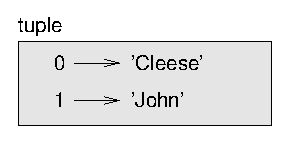
\includegraphics{figs/tuple1.eps}}
\afterfig

But in a larger diagram you might want to leave out the
details.  For example, a diagram of the telephone directory might
appear:

\beforefig
\centerline{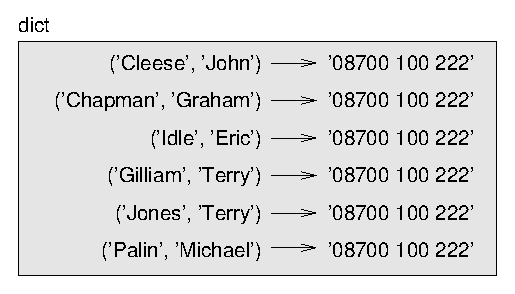
\includegraphics{figs/dict2.eps}}
\afterfig

Here the tuples are shown using Python syntax as a graphical
shorthand.
%
The telephone number in the diagram is the complaints line for the
BBC, so please don't call it.



\section{Comparing tuples}

\index{comparison!tuple}
\index{tuple!comparison}
\index{sort method}
\index{method!sort}

The relational operators work with tuples and other sequences;
Python starts by comparing the first element from each
sequence.  If they are equal, it goes on to the next elements,
and so on, until it finds elements that differ.  Subsequent
elements are not considered (even if they are really big).

\beforeverb
\begin{pycode}
>>> (0, 1, 2) < (0, 3, 4)
True
>>> (0, 1, 2000000) < (0, 3, 4)
True
\end{pycode}
\afterverb
%
The {\tt sort} function works the same way.  It sorts 
primarily by first element, but in the case of a tie, it sorts
by second element, and so on.  
%
This feature lends itself to a pattern called {\bf DSU} for 

\begin{description}

\item[Decorate] a sequence by building a list of tuples
with one or more sort keys preceding the elements from the sequence,

\item[Sort] the list of tuples, and

\item[Undecorate] by extracting the sorted elements of the sequence.

\end{description}

\label{DSU}
\index{DSU pattern}
\index{pattern!DSU}
\index{decorate-sort-undecorate pattern}
\index{pattern!decorate-sort-undecorate}

For example, suppose you have a list of words and you want to
sort them from longest to shortest:

\beforeverb
\begin{pycode}
def sort_by_length(words):
    t = []
    for word in words:
       t.append((len(word), word))

    t.sort(reverse=True)

    res = []
    for length, word in t:
        res.append(word)
    return res
\end{pycode}
\afterverb
%
The first loop builds a list of tuples, where each
tuple is a word preceded by its length.
%
{\tt sort} compares the first element, length, first, and
only considers the second element to break ties.  The keyword argument
{\tt reverse=True} tells {\tt sort} to go in decreasing order.
%
\index{keyword argument}
\index{argument!keyword}
\index{traversal}
%
The second loop traverses the list of tuples and builds a list of
words in descending order of length.

\begin{exercise}
In this example, ties are broken by comparing words, so words
with the same length appear in reverse alphabetical order.  For other
applications you might want to break ties at random.  Modify
this example so that words with the same length appear in
random order.  Hint: see the {\tt random} function in the
{\tt random} module.

\index{random module}
\index{module!random}
\index{random function}
\index{function!random}

\end{exercise}


\section{Sequences of sequences}
\index{sequence}

I have focused on lists of tuples, but almost all of the examples in
this chapter also work with lists of lists, tuples of tuples, and
tuples of lists.  To avoid enumerating the possible combinations, it
is sometimes easier to talk about sequences of sequences.
%
In many contexts, the different kinds of sequences (strings, lists and
tuples) can be used interchangeably.  So how and why do you choose one
over the others?

\index{string}
\index{list}
\index{tuple}
\index{mutability}
\index{immutability}

To start with the obvious, strings are more limited than other
sequences because the elements have to be characters.  They are
also immutable.  If you need the ability to change the characters
in a string (as opposed to creating a new string), you might
want to use a list of characters instead.

Lists are more common than tuples, mostly because they are mutable.
But there are a few cases where you might prefer tuples:

\begin{enumerate}

\item In some contexts, like a {\tt return} statement, it is
syntactically simpler to create a tuple than a list.  In other
contexts, you might prefer a list.

\item If you want to use a sequence as a dictionary key, you
have to use an immutable type like a tuple or string.

\item If you are passing a sequence as an argument to a function,
using tuples reduces the potential for unexpected behavior
due to aliasing.

\end{enumerate}

Because tuples are immutable, they don't provide methods
like {\tt sort} and {\tt reverse}, which modify existing lists.
But Python provides the built-in functions {\tt sorted}
and {\tt reversed}, which take any sequence as a parameter
and return a new list with the same elements in a different
order.

\index{sorted function}
\index{function!sorted}
\index{reversed function}
\index{function!reversed}


\section{Glossary}
	
\begin{vocabulary}[tuple:] An immutable sequence of elements.
\index{tuple}
\end{vocabulary}
	
\begin{vocabulary}[tuple assignment:] An assignment with a sequence on the
right side and a tuple of variables on the left.  The right
side is evaluated and then its elements are assigned to the
variables on the left.
\index{tuple assignment}
\index{assignment!tuple}
\end{vocabulary}
	
\begin{vocabulary}[gather:] The operation of assembling a variable-length
argument tuple.
\index{gather}
\end{vocabulary}
	
\begin{vocabulary}[scatter:] The operation of treating a sequence as a list of
arguments.
\index{scatter}
\end{vocabulary}
	
\begin{vocabulary}[DSU:] Abbreviation of ``decorate-sort-undecorate,'' a
pattern that involves building a list of tuples, sorting, and
extracting part of the result.
\index{DSU pattern}
\end{vocabulary}
	
\begin{vocabulary}[data structure:] A collection of related values, often
organized in lists, dictionaries, tuples, etc.
\index{data structure}
\end{vocabulary}
	
\begin{vocabulary}[shape (of a data structure):] A summary of the type,
size and composition of a data structure.
\index{shape}
\end{vocabulary}
	


\section{Exercises}

\begin{exercise}
Write a function called \verb"most_frequent" that takes a string and
prints the letters in decreasing order of frequency.  Find text
samples from several different languages and see how letter frequency
varies between languages.  Compare your results with the tables at
\url{wikipedia.org/wiki/Letter_frequencies}.

\index{letter frequency}
\index{frequency!letter}

\end{exercise}


\begin{exercise}
\label{anagrams}

\index{anagram set}
\index{set!anagram}

More anagrams!

\begin{enumerate}

\item Write a program
that reads a word list from a file (see Section~\ref{wordlist}) and
prints all the sets of words that are anagrams.

Here is an example of what the output might look like:

\beforeverb
\begin{pyexo}
['deltas', 'desalt', 'lasted', 'salted', 'slated', 'staled']
['retainers', 'ternaries']
['generating', 'greatening']
['resmelts', 'smelters', 'termless']
\end{pyexo}
\afterverb
%
Hint: you might want to build a dictionary that maps from a
set of letters to a list of words that can be spelled with those
letters.  The question is, how can you represent the set of
letters in a way that can be used as a key?

\item Modify the previous program so that it prints the largest set
of anagrams first, followed by the second largest set, and so on.

\index{Scrabble}
\index{bingo}

\item In Scrabble a ``bingo'' is when you play all seven tiles in
your rack, along with a letter on the board, to form an eight-letter
word.  What set of 8 letters forms the most possible bingos?
Hint: there are seven.

% (7, ['angriest', 'astringe', 'ganister', 'gantries', 'granites',
% 'ingrates', 'rangiest'])

\index{metathesis}

\item Two words form a ``metathesis pair'' if you can transform one
  into the other by swapping two letters\footnote{This exercise is
    inspired by an example at \url{puzzlers.org}.}; for example,
  ``converse'' and ``conserve.''  Write a program that finds all of
  the metathesis pairs in the dictionary.  Hint: don't test all pairs
  of words, and don't test all possible swaps.

You can download a solution from \url{thinkpython.com/code/anagram_sets.py}.

\end{enumerate}
\end{exercise}



\begin{exercise}

\index{Car Talk}
\index{Puzzler}

Here's another Car Talk Puzzler\footnote{
\url{www.cartalk.com/content/puzzler/transcripts/200651}.}:

\begin{quote}
What is the longest English word, that remains a valid English word,
as you remove its letters one at a time?

Now, letters can be removed from either end, or the middle, but you
can't rearrange any of the letters. Every time you drop a letter, you
wind up with another English word. If you do that, you're eventually
going to wind up with one letter and that too is going to be an
English word---one that's found in the dictionary. I want to know
what's the longest word and how many letters does it
have?

I'm going to give you a little modest example: Sprite. Ok? You start
off with sprite, you take a letter off, one from the interior of the
word, take the r away, and we're left with the word spite, then we
take the e off the end, we're left with spit, we take the s off, we're
left with pit, it, and I.
\end{quote}

\index{reducible word}
\index{word, reducible}

Write a program to find all words that can be reduced in this way,
and then find the longest one.

This exercise is a little more challenging than most, so here are
some suggestions:

\begin{enumerate}

\item You might want to write a function that takes a word and
  computes a list of all the words that can be formed by removing one
  letter.  These are the ``children'' of the word.

\index{recursive definition}
\index{definition!recursive}

\item Recursively, a word is reducible if any of its children
are reducible.  As a base case, you can consider the empty
string reducible.

\item The wordlist I provided, {\tt words.txt}, doesn't
contain single letter words.  So you might want to add
``I'', ``a'', and the empty string.

\item To improve the performance of your program, you might want
to memorize the words that are known to be reducible.

\end{enumerate}

You can see my solution at \url{thinkpython.com/code/reducible.py}.

\end{exercise}




%\begin{ex}
%\url{wikipedia.org/wiki/Word_Ladder}
%\end{ex}





%\chapterimage{chapter_head_1.pdf} % Chapter heading image
\chapter{Files}

\index{file}
\index{type!file}


\section{Persistence}

\index{persistence}

Most of the programs we have seen so far are transient in the
sense that they run for a short time and produce some output,
but when they end, their data disappears.  If you run the program
again, it starts with a clean slate.

Other programs are {\bf persistent}: they run for a long time
(or all the time); they keep at least some of their data
in permanent storage (a hard drive, for example); and
if they shut down and restart, they pick up where they left off.
%
Examples of persistent programs are operating systems, which
run pretty much whenever a computer is on, and web servers,
which run all the time, waiting for requests to come in on
the network.
%
One of the simplest ways for programs to maintain their data
is by reading and writing text files. A text file is a sequence
of characters stored on a permanent medium like a hard drive, 
flash memory, or CD-ROM. 


\section{Reading from a file}
\label{wordlist}

In this chapter we will be using a list of English words.
There are lots of word lists available on the Web, but the one most
suitable for our purpose is one of the word lists collected and
contributed to the public domain by Grady Ward as part of the Moby
lexicon project\footnote{\url{wikipedia.org/wiki/Moby_Project}.}.  It
is a list of 113,809 official crosswords; that is, words that are
considered valid in crossword puzzles and other word games.  In the
Moby collection, the filename is {\tt 113809of.fic}; I include a copy
of this file, with the simpler name {\tt words.txt}, along with
Swampy.

\index{Swampy}
\index{crosswords}

This file is in plain text, so you can open it with a text
editor, but you can also read it from Python.  The built-in
function {\tt open} takes the name of the file as a parameter
and returns a {\bf file object} you can use to read the file.

\index{open function}
\index{function!open}
\index{plain text}
\index{text!plain}
\index{object!file}
\index{file object}

\beforeverb
\begin{pyinterpreter}
>>> fin = open('words.txt')
>>> print(fin)
<open file 'words.txt', mode 'r' at 0xb7f4b380>
\end{pyinterpreter}
\afterverb
%
{\tt fin} is a common name for a file object used for
input.  Mode \verb"'r'" indicates that this file is open for
reading (as opposed to \verb"'w'" for writing).

\index{readline method}
\index{method!readline}

The file object provides several methods for reading, including
{\tt readline}, which reads characters from the file
until it gets to a newline and returns the result as a
string:

\beforeverb
\begin{pyinterpreter}
>>> fin.readline()
'aa\r\n'
\end{pyinterpreter}
\afterverb
%
The first word in this particular list is ``aa,'' which is a kind of
lava.  The sequence \verb"\r\n" represents two whitespace characters,
a carriage return and a newline, that separate this word from the
next.

The file object keeps track of where it is in the file, so
if you call {\tt readline} again, you get the next word:

\beforeverb
\begin{pyinterpreter}
>>> fin.readline()
'aah\r\n'
\end{pyinterpreter}
\afterverb
%
The next word is ``aah,'' which is, believe it or not, a perfectly legitimate
word. If the whitespace is bothering you,
we can get rid of it with the string method {\tt strip}:

\index{strip method}
\index{method!strip}

\beforeverb
\begin{pyinterpreter}
>>> line = fin.readline()
>>> word = line.strip()
>>> print(word)
aahed
\end{pyinterpreter}
\afterverb
%
You can also use a file object as part of a {\tt for} loop.
This program reads {\tt words.txt} and prints each word, one
per line:

\index{open function}
\index{function!open}

\beforeverb
\begin{pycode}
fin = open('words.txt')
for line in fin:
    word = line.strip()
    print(word)
\end{pycode}
\afterverb
%

\section{Writing to a file}

\index{file!writing}

\index{open function}
\index{function!open}

To write a file, you have to open it with mode
\verb"'w'" as a second parameter:

\beforeverb
\begin{pyinterpreter}
>>> fout = open('output.txt', 'w')
>>> print(fout)
<open file 'output.txt', mode 'w' at 0xb7eb2410>
\end{pyinterpreter}
\afterverb
%
If the file already exists, opening it in write mode clears out
the old data and starts fresh, so be careful!
If the file doesn't exist, a new one is created.

The {\tt write} method puts data into the file.

\beforeverb
\begin{pyinterpreter}
>>> line1 = "This here's the wattle,\n"
>>> fout.write(line1)
\end{pyinterpreter}
\afterverb
%
Again, the file object keeps track of where it is, so if
you call {\tt write} again, it adds the new data to the end.

\beforeverb
\begin{pyinterpreter}
>>> line2 = "the emblem of our land.\n"
>>> fout.write(line2)
\end{pyinterpreter}
\afterverb
%
When you are done writing, you have to close the file.

\beforeverb
\begin{pyinterpreter}
>>> fout.close()
\end{pyinterpreter}
\afterverb
%

\index{close method}
\index{method!close}


\section{Format operator}

\index{format operator}
\index{operator!format}

The argument of {\tt write} has to be a string, so if we want
to put other values in a file, we have to convert them to
strings.  The easiest way to do that is with {\tt str}:

\beforeverb
\begin{pyinterpreter}
>>> x = 52
>>> f.write(str(x))
\end{pyinterpreter}
\afterverb
%
An alternative is to use the {\bf format operator}, {\tt \%}.  When
applied to integers, {\tt \%} is the modulus operator.  But
when the first operand is a string, {\tt \%} is the format operator.

\index{format string}

The first operand is the {\bf format string}, which contains
one or more {\bf format sequences}, which
specify how
the second operand is formatted.  The result is a string.

\index{format sequence}

For example, the format sequence \verb"'%d'" means that
the second operand should be formatted as an
integer ({\tt d} stands for ``decimal''):

\beforeverb
\begin{pyinterpreter}
>>> camels = 42
>>> '%d' % camels
'42'
\end{pyinterpreter}
\afterverb
%
The result is the string \verb"'42'", which is not to be confused
with the integer value {\tt 42}.

A format sequence can appear anywhere in the string,
so you can embed a value in a sentence:

\beforeverb
\begin{pyinterpreter}
>>> camels = 42
>>> 'I have spotted %d camels.' % camels
'I have spotted 42 camels.'
\end{pyinterpreter}
\afterverb
%
If there is more than one format sequence in the string,
the second argument has to be a tuple.  Each format sequence is
matched with an element of the tuple, in order.

The following example uses \verb"'%d'" to format an integer,
\verb"'%g'" to format
a floating-point number (don't ask why), and \verb"'%s'" to format
a string:

\beforeverb
\begin{pyinterpreter}
>>> 'In %d years I have spotted %g %s.' % (3, 0.1, 'camels')
'In 3 years I have spotted 0.1 camels.'
\end{pyinterpreter}
\afterverb
%
The number of elements in the tuple has to match the number
of format sequences in the string.  Also, the types of the
elements have to match the format sequences:

\index{exception!TypeError}
\index{TypeError}

\beforeverb
\begin{pyinterpreter}
>>> '%d %d %d' % (1, 2)
TypeError: not enough arguments for format string
>>> '%d' % 'dollars'
TypeError: illegal argument type for built-in operation
\end{pyinterpreter}
\afterverb
%
In the first example, there aren't enough elements; in the
second, the element is the wrong type.

The format operator is powerful, but it can be difficult to use.  You
can read more about it at
\url{docs.python.org/lib/typesseq-strings.html}.

% You can specify the number of digits as part of the format sequence.
% For example, the sequence \verb"'%8.2f'"
% formats a floating-point number to be 8 characters long, with
% 2 digits after the decimal point:

% \beforeverb
% \begin{pyinterpreter}
% >>> '%8.2f' % 3.14159
% '    3.14'
% \end{pyinterpreter}
% \afterverb
% %
% The result takes up eight spaces with two
% digits after the decimal point.  


\section{Filenames and paths}
\label{paths}

\index{filename}
\index{path}
\index{directory}
\index{folder}

Files are organized into {\bf directories} (also called ``folders'').
Every running program has a ``current directory,'' which is the
default directory for most operations.  
For example, when you open a file for reading, Python looks for it in the
current directory.

\index{os module}
\index{module!os}

The {\tt os} module provides functions for working with files and
directories (``os'' stands for ``operating system'').  {\tt os.getcwd}
returns the name of the current directory:

\index{getcwd function}
\index{function!getcwd}

\beforeverb
\begin{pyinterpreter}
>>> import os
>>> cwd = os.getcwd()
>>> print(cwd)
/home/dinsdale
\end{pyinterpreter}
\afterverb
%
{\tt cwd} stands for ``current working directory.''  The result in
this example is {\tt /home/dinsdale}, which is the home directory of a
user named {\tt dinsdale}.

\index{working directory}
\index{directory!working}

A string like {\tt cwd} that identifies a file is called a {\bf path}.
A {\bf relative path} starts from the current directory;
an {\bf absolute path} starts from the topmost directory in the
file system.

\index{relative path}
\index{path!relative}
\index{absolute path}
\index{path!absolute}

The paths we have seen so far are simple filenames, so they are
relative to the current directory.  To find the absolute path to
a file, you can use {\tt os.path.abspath}:

\beforeverb
\begin{pyinterpreter}
>>> os.path.abspath('memo.txt')
'/home/dinsdale/memo.txt'
\end{pyinterpreter}
\afterverb
%
{\tt os.path.exists} checks
whether a file or directory exists:

\index{exists function}
\index{function!exists}

\beforeverb
\begin{pyinterpreter}
>>> os.path.exists('memo.txt')
True
\end{pyinterpreter}
\afterverb
%
If it exists, {\tt os.path.isdir} checks whether it's a directory:

\beforeverb
\begin{pyinterpreter}
>>> os.path.isdir('memo.txt')
False
>>> os.path.isdir('music')
True
\end{pyinterpreter}
\afterverb
%
Similarly, {\tt os.path.isfile} checks whether it's a file.

{\tt os.listdir} returns a list of the files (and other directories)
in the given directory:

\beforeverb
\begin{pyinterpreter}
>>> os.listdir(cwd)
['music', 'photos', 'memo.txt']
\end{pyinterpreter}
\afterverb
%
To demonstrate these functions, the following example
``walks'' through a directory, prints
the names of all the files, and calls itself recursively on
all the directories.

\index{walk, directory}
\index{directory!walk}

\beforeverb
\begin{pycode}
def walk(dir):
    for name in os.listdir(dir):
        path = os.path.join(dir, name)

        if os.path.isfile(path):
            print(path)
        else:
            walk(path)
\end{pycode}
\afterverb
%
{\tt os.path.join} takes a directory and a file name and joins
them into a complete path.  

\begin{exercise}
Modify {\tt walk} so that instead of printing the names of
the files, it returns a list of names.
\end{exercise}

\begin{exercise}
The {\tt os} module provides a function called {\tt walk}
that is similar to this one but more versatile.  Read
the documentation and use it to print the names of the
files in a given directory and its subdirectories.
\end{exercise}


\section{Catching exceptions}
\label{catch}

A lot of things can go wrong when you try to read and write
files.  If you try to open a file that doesn't exist, you get an
{\tt IOError}:

\index{open function}
\index{function!open}
\index{exception!IOError}
\index{IOError}

\beforeverb
\begin{pyinterpreter}
>>> fin = open('bad_file')
IOError: [Errno 2] No such file or directory: 'bad_file'
\end{pyinterpreter}
\afterverb
%
If you don't have permission to access a file:

\index{file!permission}
\index{permission, file}

\beforeverb
\begin{pyinterpreter}
>>> fout = open('/etc/passwd', 'w')
IOError: [Errno 13] Permission denied: '/etc/passwd'
\end{pyinterpreter}
\afterverb
%
And if you try to open a directory for reading, you get

\beforeverb
\begin{pyinterpreter}
>>> fin = open('/home')
IOError: [Errno 21] Is a directory
\end{pyinterpreter}
\afterverb
%
To avoid these errors, you could use functions like {\tt os.path.exists}
and {\tt os.path.isfile}, but it would take a lot of time and code
to check all the possibilities (if ``{\tt Errno 21}'' is any
indication, there are at least 21 things that can go wrong).

\index{exception, catching}
\index{try statement}
\index{statement!try}

It is better to go ahead and try, and deal with problems if they
happen, which is exactly what the {\tt try} statement does.  The
syntax is similar to an {\tt if} statement:

\beforeverb
\begin{pycode}
try:    
    fin = open('bad_file')
    for line in fin:
        print(line)
    fin.close()
except:
    print('Something went wrong.')
\end{pycode}
\afterverb
%
Python starts by executing the {\tt try} clause.  If all goes
well, it skips the {\tt except} clause and proceeds.  If an
exception occurs, it jumps out of the {\tt try} clause and
executes the {\tt except} clause.

Handling an exception with a {\tt try} statement is called {\bf
catching} an exception.  In this example, the {\tt except} clause
prints an error message that is not very helpful.  In general,
catching an exception gives you a chance to fix the problem, or try
again, or at least end the program gracefully.


\subsection{{\tt finally} clause}
There are two options to the \verb|try-except| statement.
The first one is the clause {\tt finally}. All code included in the 
{\tt finally} clause will be executed, whether an exception occurred 
or not. This is a good place to clean up our program. For example
this is a good place to close a file if it has been open in the {\tt try} 
clause. The code below shows how it is done.


\beforeverb
\begin{pycode}
fin = None
try:    
    print('Try to open a file.')
    fin = open('words.txt')
    for line in fin:
        print(line)
except:
    print('Something went wrong.')
finally:
    print('cleaning up')
    if fin is not None:
        print('closing the file')
        fin.close()
\end{pycode}
\afterverb

First we set the variable {\tt fin} to {\tt None}. In the {\tt try} clause, we 
open a file and then assign it to {\tt fin}. Two things can happen:

\begin{itemize}
	\item An exception occurs while we
are trying to open the file, {\tt fin} is not assigned any new object and contains 
the value {\tt None}. The program jumps directly to the {\tt except} clause and
executes the code in the {\tt except} block. Then the program jumps to the {\tt finally} 
clause and executes the code there.

	\item The file is opened successfully, {\tt fin} is assigned the file object, and the rest
	of the code in the {\tt try} statement is executed. Then the program jumps to the {\tt finally}
	clause and executes the code there.

\end{itemize} 

\subsection{{\tt else} clause}
The second option is the {\tt else} clause, which should be after the {\tt except} clause and before the {\tt finally} clause. The code in the {\tt else} clause is executed only if no exceptions were raised. It is executed before the {\tt finally} clause. The {\tt else} clause is use for all code that does not raise any exception. In our previous code, it would be the place to read the lines in the file. The refactored code is:

\beforeverb
\begin{pycode}
fin = None
try:    
    fin = open('word.txt')
except:
    print('Something went wrong.')
else:
    print('Do your thing if all went well.')
    for line in fin:
        print(line)    
finally:
    print('cleaning up.')
    if fin is not None:
        print('closing the file.')
        fin.close()
\end{pycode}
\afterverb

As you can see, the {\tt try} clause contains only the code that may raise an exception. 
\begin{itemize}
	\item If an exception occurs whilst opening the file, the program jumps to the {\tt except} clause and then executes the {\tt finally} clause. In this case, the output is: 

\begin{pyoutput}
TRY: open file.
EXCEPT: Something went wrong.
FINALLY: cleaning up.
\end{pyoutput}

	\item If no exceptions are raised, the program skips the {\tt except} clause, and jumps to the {\tt else} clause. Once the code in the {\tt else} clause has been executed, the program jumps to the {\tt finally} clause. In this case, the output is: 

\begin{pyoutput}
TRY: open file.
--> file open successfully.
ELSE: Do your thing if all went well.
--> line 1 of text file

--> line 2 of text file

--> last line of text file

FINALLY: cleaning up.
--> closing the file.
\end{pyoutput}

\end{itemize} 

\section{Writing modules}
\label{modules}

\index{module, writing}
\index{word count}

Any file that contains Python code can be imported as a module.
For example, suppose you have a file named {\tt wc.py} with the following
code:

\beforeverb
\begin{pycode}
def linecount(filename):
    count = 0
    for line in open(filename):
        count += 1
    return count

print(linecount('wc.py'))
\end{pycode}
\afterverb
%
If you run this program, it reads itself and prints the number
of lines in the file, which is 7.
You can also import it like this:

\beforeverb
\begin{pyinterpreter}
>>> import wc
7
\end{pyinterpreter}
\afterverb
%
Now you have a module object {\tt wc}:

\index{module object}
\index{object!module}

\beforeverb
\begin{pyinterpreter}
>>> print(wc)
<module 'wc' from 'wc.py'>
\end{pyinterpreter}
\afterverb
%
That provides a function called \verb"linecount":

\beforeverb
\begin{pyinterpreter}
>>> wc.linecount('wc.py')
7
\end{pyinterpreter}
\afterverb
%
So that's how you write modules in Python.

The only problem with this example is that when you import
the module it executes the test code at the bottom.  Normally
when you import a module, it defines new functions but it
doesn't execute them.

\index{import statement}
\index{statement!import}

Programs that will be imported as modules often
use the following idiom:

\beforeverb
\begin{pycode}
if __name__ == '__main__':
    print(linecount('wc.py'))
\end{pycode}
\afterverb
%
\verb"__name__" is a built-in variable that is set when the
program starts.  If the program is running as a script,
\verb"__name__" has the value \verb"__main__"; in that
case, the test code is executed.  Otherwise,
if the module is being imported, the test code is skipped.

\begin{exercise}
Type this example into a file named {\tt wc.py} and run
it as a script.  Then run the Python interpreter and
{\tt import wc}.  What is the value of \verb"__name__"
when the module is being imported?

Warning: If you import a module that has already been imported,
Python does nothing.  It does not re-read the file, even if it has
changed.

\index{module!reload}
\index{reload function}
\index{function!reload}

If you want to reload a module, you can use the built-in function 
{\tt reload}, but it can be tricky, so the safest thing to do is
restart the interpreter and then import the module again.
\end{exercise}



\section{Debugging}

\index{debugging}
\index{whitespace}

When you are reading and writing files, you might run into problems
with whitespace.  These errors can be hard to debug because spaces,
tabs and newlines are normally invisible:

\beforeverb
\begin{pyinterpreter}
>>> s = '1 2\t 3\n 4'
>>> print(s)
1 2	 3
 4
\end{pyinterpreter}
\afterverb

\index{repr function}
\index{function!repr}
\index{string representation}

The built-in function {\tt repr} can help.  It takes any object as an
argument and returns a string representation of the object.  For
strings, it represents whitespace
characters with backslash sequences:

\beforeverb
\begin{pyinterpreter}
>>> print(repr(s))
'1 2\t 3\n 4'
\end{pyinterpreter}
\afterverb

This can be helpful for debugging.

One other problem you might run into is that different systems
use different characters to indicate the end of a line.  Some
systems use a newline, represented \verb"\n".  Others use
a return character, represented \verb"\r".  Some use both.
If you move files between different systems, these inconsistencies
might cause problems.

\index{end of line character}

For most systems, there are applications to convert from one
format to another.  You can find them (and read more about this
issue) at \url{wikipedia.org/wiki/Newline}.  Or, of course, you
could write one yourself.


\section{Glossary}
	
\begin{vocabulary}[persistent:] Pertaining to a program that runs indefinitely
and keeps at least some of its data in permanent storage.
\index{persistence}
\end{vocabulary}
	
\begin{vocabulary}[format operator:] An operator, {\tt \%}, that takes a format
string and a tuple and generates a string that includes
the elements of the tuple formatted as specified by the format string.
\index{format operator}
\index{operator!format}
\end{vocabulary}
	
\begin{vocabulary}[format string:] A string, used with the format operator, that
contains format sequences.  
\index{format string}
\end{vocabulary}
	
\begin{vocabulary}[format sequence:] A sequence of characters in a format string,
like {\tt \%d}, that specifies how a value should be formatted.
\index{format sequence}
\end{vocabulary}
	
\begin{vocabulary}[text file:] A sequence of characters stored in permanent
storage like a hard drive.
\index{text file}
\end{vocabulary}
	
\begin{vocabulary}[directory:] A named collection of files, also called a folder.
\index{directory}
\end{vocabulary}
	
\begin{vocabulary}[path:] A string that identifies a file.
\index{path}
\end{vocabulary}
	
\begin{vocabulary}[relative path:] A path that starts from the current directory.
\index{relative path}
\end{vocabulary}
	
\begin{vocabulary}[absolute path:] A path that starts from the topmost directory
in the file system.
\index{absolute path}
\end{vocabulary}
	
\begin{vocabulary}[catch:] To prevent an exception from terminating
a program using the {\tt try}
and {\tt except} statements.
\end{vocabulary}


\section{Exercises}
\label{sec:files-exercises}

\begin{exercise}
\label{urllib}

\index{urllib module}
\index{module!urllib}
\index{URL}

The {\tt urllib} module provides methods for manipulating URLs
and downloading information from the web.  The following example
downloads and prints a secret message from {\tt thinkpython.com}:

\beforeverb
\begin{pyexo}
import urllib

conn = urllib.urlopen('http://thinkpython.com/secret.html')
for line in conn.fp:
    print(line.strip())
\end{pyexo}
\afterverb

Run this code and follow the instructions you see there.

\index{secret exercise}
\index{exercise, secret}

\end{exercise}

\begin{exercise}
\label{ex:words-file}
Write a program that reads {\tt words.txt} and prints only the
words with more than 20 characters (not counting whitespace).

\index{whitespace}

\end{exercise}

\begin{exercise}
\label{ex:gadsby}
In 1939 Ernest Vincent Wright published a 50,000 word novel called
{\em Gadsby} that does not contain the letter ``e.''  Since ``e'' is
the most common letter in English, that's not easy to do.

In fact, it is difficult to construct a solitary thought without using
that most common symbol.  It is slow going at first, but with caution
and hours of training you can gradually gain facility.

All right, I'll stop now.

Write a function called \verb"has_no_e" that returns {\tt True} if
the given word doesn't have the letter ``e'' in it.

Modify your program from the previous section to print only the words
that have no ``e'' and compute the percentage of the words in the list
have no ``e.''

\index{lipogram}

\end{exercise}


\begin{exercise} 
\label{ex:avoids}
Write a function named {\tt avoids}
that takes a word and a string of forbidden letters, and
that returns {\tt True} if the word doesn't use any of the forbidden
letters.

Modify your program to prompt the user to enter a string
of forbidden letters and then print the number of words that
don't contain any of them.
Can you find a combination of 5 forbidden letters that
excludes the smallest number of words?
\end{exercise}



\begin{exercise}
\label{ex:uses-only}

Write a function named \verb"uses_only" that takes a word and a
string of letters, and that returns {\tt True} if the word contains
only letters in the list.  Can you make a sentence using only the
letters {\tt acefhlo}?  Other than ``Hoe alfalfa?''
\end{exercise}


\begin{exercise} 
\label{ex:uses-all}

Write a function named \verb"uses_all" that takes a word and a
string of required letters, and that returns {\tt True} if the word
uses all the required letters at least once.  How many words are there
that use all the vowels {\tt aeiou}?  How about {\tt aeiouy}?
\end{exercise}


\begin{exercise}
\label{ex:abecedarian}

Write a function called \verb"is_abecedarian" that returns
{\tt True} if the letters in a word appear in alphabetical order
(double letters are ok).  
How many abecedarian words are there?
\end{exercise}

\index{abecedarian}


\begin{exercise}
\label{ex:palindrome}
A palindrome is a word that reads the same
forward and backward, like ``rotator'' and ``noon.''
Write a boolean function named \verb"is_palindrome" that
takes a string as a parameter and returns {\tt True} if it is
a palindrome.

Modify your program from the previous section to print all
of the palindromes in the word list and then print the total
number of palindromes.
\end{exercise}



%\input{./Chapters/Chapter_recursion}

%\input{./Chapters/Chapter_recap_problem}

%\input{./Chapters/Chapter_interfaces}

\part{Part III - Object Oriented Programming}
\chapterimage{chapter_head_1.pdf} % Chapter heading image
\chapter{Classes and objects}


\section{User-defined types}
\label{point}

\index{user-defined type}
\index{type!user-defined}

We have used many of Python's built-in types; now we are going
to define a new type.  As an example, we will create a type
called {\tt Point} that represents a point in two-dimensional
space.
%
\index{point, mathematical}
%
In mathematical notation, points are often written in
parentheses with a comma separating the coordinates. For example,
$(0, 0)$ represents the origin, and $(x, y)$ represents the
point $x$ units to the right and $y$ units up from the origin.

There are several ways we might represent points in Python:

\begin{itemize}

\item We could store the coordinates separately in two
variables, {\tt x} and {\tt y}.

\item We could store the coordinates as elements in a list
or tuple.

\item We could create a new type to represent points as
objects.

\end{itemize}

\index{representation}

Creating a new type
is (a little) more complicated than the other options, but
it has advantages that will be apparent soon.
%
A user-defined type is also called a {\bf class}.
A class definition looks like this:

\index{class}
\index{object}
\index{class definition}
\index{definition!class}

\beforeverb
\begin{pycode}
class Point(object):
    """represents a point in 2-D space"""
\end{pycode}
\afterverb
%
This header indicates that the new class is a {\tt Point},
which is a kind of {\tt object}, which is a built-in
type.
%
\index{Point class}
\index{class!Point}
%
The body is a docstring that explains what the class is for.
You can define variables and functions inside a class definition,
but we will get back to that later.

\index{docstring}

Defining a class named {\tt Point} creates a class object.

\beforeverb
\begin{pyinterpreter}
>>> print(Point)
<class '__main__.Point'>
\end{pyinterpreter}
\afterverb
%
Because {\tt Point} is defined at the top level, its ``full
name'' is \verb"__main__.Point".
%
\index{object!class}
\index{class object}
%
The class object is like a factory for creating objects.  To create a
Point, you call {\tt Point} as if it were a function.

\beforeverb
\begin{pyinterpreter}
>>> blank = Point()
>>> print(blank)
<__main__.Point instance at 0xb7e9d3ac>
\end{pyinterpreter}
\afterverb
%
The return value is a reference to a Point object, which we
assign to {\tt blank}.  
Creating a new object is called
{\bf instantiation}, and the object is an {\bf instance} of
the class.
%
\index{instance}
\index{instantiation}
%
When you print an instance, Python tells you what class it
belongs to and where it is stored in memory (the prefix
{\tt 0x} means that the following number is in hexadecimal).

\index{hexadecimal}


\section{Attributes}

\index{instance attribute}
\index{attribute!instance}
\index{dot notation}

You can assign values to an instance using dot notation:

\beforeverb
\begin{pyinterpreter}
>>> blank.x = 3.0
>>> blank.y = 4.0
\end{pyinterpreter}
\afterverb
%
This syntax is similar to the syntax for selecting a variable from a
module, such as {\tt math.pi} or {\tt string.whitespace}.  In this case,
though, we are assigning values to named elements of an object.
These elements are called {\bf attributes}.
%
As a noun, ``AT-trib-ute'' is pronounced with emphasis on the first
syllable, as opposed to ``a-TRIB-ute,'' which is a verb.
%
The following diagram shows the result of these assignments.
A state diagram that shows an object and its attributes is
called an {\bf object diagram}:

\index{state diagram}
\index{diagram!state}
\index{object diagram}
\index{diagram!object}

\beforefig
\centerline{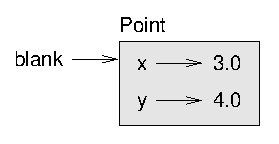
\includegraphics{figs/point.eps}}
\afterfig

The variable {\tt blank} refers to a Point object, which
contains two attributes.  Each attribute refers to a
floating-point number.
%
You can read the value of an attribute using the same syntax:

\beforeverb
\begin{pyinterpreter}
>>> print(blank.y)
4.0
>>> x = blank.x
>>> print(x)
3.0
\end{pyinterpreter}
\afterverb
%
The expression {\tt blank.x} means, ``Go to the object {\tt blank}
refers to and get the value of {\tt x}.'' In this case, we assign that
value to a variable named {\tt x}.  There is no conflict between
the variable {\tt x} and the attribute {\tt x}.

You can use dot notation as part of any expression.  For example:

\beforeverb
\begin{pyinterpreter}
>>> print('(%g, %g)' % (blank.x, blank.y))
(3.0, 4.0)
>>> distance = math.sqrt(blank.x**2 + blank.y**2)
>>> print(distance)
5.0
\end{pyinterpreter}
\afterverb
%
You can pass an instance as an argument in the usual way.
For example:

\index{instance!as argument}

\beforeverb
\begin{pycode}
def print_point(p):
    print('(%g, %g)' % (p.x, p.y))
\end{pycode}
\afterverb
%
\verb"print_point" takes a point as an argument and displays it in
mathematical notation.  To invoke it, you can pass {\tt blank} as
an argument:

\beforeverb
\begin{pyinterpreter}
>>> print_point(blank)
(3.0, 4.0)
\end{pyinterpreter}
\afterverb
%
Inside the function, {\tt p} is an alias for {\tt blank}, so if
the function modifies {\tt p}, {\tt blank} changes.

\index{aliasing}


\begin{exercise}
Write a function called {\tt distance} that takes two Points
as arguments and returns the distance between them. The distance between
two points $A=(x_A, y_A)$ and $B=(x_B, y_B)$ is given by:
\begin{equation}
d(A,B) = \sqrt{(x_A - x_B)^2 + (y_A - y_B)^2}
\label{eq:distance}
\end{equation}
\end{exercise}



\section{Rectangles}

Sometimes it is obvious what the attributes of an object should be,
but other times you have to make decisions.  For example, imagine you
are designing a class to represent rectangles.  What attributes would
you use to specify the location and size of a rectangle?  You can
ignore angle; to keep things simple, assume that the rectangle is
either vertical or horizontal.

\index{representation}

There are at least two possibilities: 

\begin{itemize}

\item You could specify one corner of the rectangle
(or the center), the width, and the height.

\item You could specify two opposing corners.

\end{itemize}

At this point it is hard to say whether either is better than
the other, so we'll implement the first one, just as an example.

\index{Rectangle class}
\index{class!Rectangle}

Here is the class definition:

\beforeverb
\begin{pycode}
class Rectangle(object):
    """represent a rectangle. 
       attributes: width, height, corner (bottom left corner).
    """
\end{pycode}
\afterverb
%
The docstring lists the attributes:  {\tt width} and
{\tt height} are numbers; {\tt corner} is a Point object that
specifies the lower-left corner.
%
To represent a rectangle, you have to instantiate a Rectangle
object and assign values to the attributes:

\beforeverb
\begin{pycode}
box = Rectangle()
box.width = 100.0
box.height = 200.0
box.corner = Point()
box.corner.x = 0.0
box.corner.y = 0.0
\end{pycode}
\afterverb
%
The expression {\tt box.corner.x} means,
``Go to the object {\tt box} refers to and select the attribute named
{\tt corner}; then go to that object and select the attribute named
{\tt x}.''

The figure shows the state of this object:

\index{state diagram}
\index{diagram!state}
\index{object diagram}
\index{diagram!object}

\beforefig
\centerline{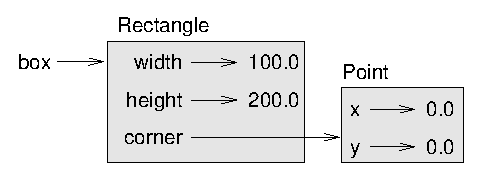
\includegraphics{figs/rectangle.eps}}
\afterfig

An object that is an attribute of another object is {\bf embedded}.

\index{embedded object}
\index{object!embedded}


\section{Instances as return values}

\index{instance!as return value}
\index{return value}

Functions can return instances.  For example, \verb"find_center"
takes a {\tt Rectangle} as an argument and returns a {\tt Point}
that contains the coordinates of the center of the {\tt Rectangle}:

\beforeverb
\begin{pycode}
def find_center(box):
    p = Point()
    p.x = box.corner.x + box.width/2.0
    p.y = box.corner.y + box.height/2.0
    return p
\end{pycode}
\afterverb
%
Here is an example that passes {\tt box} as an argument and assigns
the resulting Point to {\tt center}:

\beforeverb
\begin{pyinterpreter}
>>> center = find_center(box)
>>> print_point(center)
(50.0, 100.0)
\end{pyinterpreter}
\afterverb
%

\section{Objects are mutable}

\index{object!mutable}
\index{mutability}

You can change the state of an object by making an assignment to one of
its attributes.  For example, to change the size of a rectangle
without changing its position, you can modify the values of {\tt
width} and {\tt height}:

\beforeverb
\begin{pycode}
box.width = box.width + 50
box.height = box.width + 100
\end{pycode}
\afterverb
%
You can also write functions that modify objects.  For example,
\verb"grow_rectangle" takes a Rectangle object and two numbers,
{\tt dwidth} and {\tt dheight}, and adds the numbers to the
width and height of the rectangle:

\beforeverb
\begin{pycode}
def grow_rectangle(rect, dwidth, dheight) :
    rect.width += dwidth
    rect.height += dheight
\end{pycode}
\afterverb
%
Here is an example that demonstrates the effect:

\beforeverb
\begin{pyinterpreter}
>>> print(box.width)
100.0
>>> print(box.height)
200.0
>>> grow_rectangle(box, 50, 100)
>>> print(box.width)
150.0
>>> print(box.height)
300.0
\end{pyinterpreter}
\afterverb
%
Inside the function, {\tt rect} is an
alias for {\tt box}, so if the function modifies {\tt rect}, 
{\tt box} changes.

\begin{exercise}
Write a function named \verb"move_rectangle" that takes
a Rectangle and two numbers named {\tt dx} and {\tt dy}.  It
should change the location of the rectangle by adding {\tt dx}
to the {\tt x} coordinate of {\tt corner} and adding {\tt dy}
to the {\tt y} coordinate of {\tt corner}.
\end{exercise}


\section{Copying}

\index{aliasing}

Aliasing can make a program difficult to read because changes
in one place might have unexpected effects in another place.
It is hard to keep track of all the variables that might refer
to a given object.

\index{copying objects}
\index{object!copying}
\index{copy module}
\index{module!copy}

Copying an object is often an alternative to aliasing.
The {\tt copy} module contains a function called {\tt copy} that
can duplicate any object:

\beforeverb
\begin{pyinterpreter}
>>> p1 = Point()
>>> p1.x = 3.0
>>> p1.y = 4.0

>>> import copy
>>> p2 = copy.copy(p1)
\end{pyinterpreter}
\afterverb
%
{\tt p1} and {\tt p2} contain the same data, but they are
not the same Point.

\beforeverb
\begin{pyinterpreter}
>>> print_point(p1)
(3.0, 4.0)
>>> print_point(p2)
(3.0, 4.0)
>>> p1 is p2
False
>>> p1 == p2
False
\end{pyinterpreter}
\afterverb
%
The {\tt is} operator indicates that {\tt p1} and {\tt p2} are not the
same object, which is what we expected.  But you might have expected
{\tt ==} to yield {\tt True} because these points contain the same
data.  In that case, you will be disappointed to learn that for
instances, the default behavior of the {\tt ==} operator is the same
as the {\tt is} operator; it checks object identity, not object
equivalence.  Thankfully, this behavior can be changed---we'll see how later.

\index{is operator}
\index{operator!is}

If you use {\tt copy.copy} to duplicate a Rectangle, you will find
that it copies the Rectangle object but not the embedded Point.

\index{embedded object!copying}

\beforeverb
\begin{pyinterpreter}
>>> box2 = copy.copy(box)
>>> box2 is box
False
>>> box2.corner is box.corner
True
\end{pyinterpreter}
\afterverb
%
Here is what the object diagram looks like:

\index{state diagram}
\index{diagram!state}
\index{object diagram}
\index{diagram!object}

\vspace{0.1in}
\beforefig
\centerline{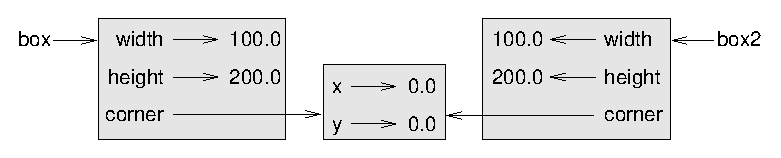
\includegraphics{figs/rectangle2.eps}}
\afterfig
\vspace{0.1in}

This operation is called a {\bf shallow copy} because it copies the
object and any references it contains, but not the embedded objects.
%
\index{shallow copy}
\index{copy!shallow}
%
For most applications, this is not what you want.  In this example,
invoking \verb"grow_rectangle" on one of the Rectangles would not
affect the other, but invoking \verb"move_rectangle" on either would
affect both!  This behavior is confusing and error-prone.
%
\index{deep copy}
\index{copy!deep}
%
Fortunately, the {\tt copy} module contains a method named {\tt
deepcopy} that copies not only the object but also 
the objects it refers to, and the objects {\em they} refer to,
and so on.
You will not be surprised to learn that this operation is
called a {\bf deep copy}.

\index{deepcopy function}
\index{function!deepcopy}

\beforeverb
\begin{pyinterpreter}
>>> box3 = copy.deepcopy(box)
>>> box3 is box
False
>>> box3.corner is box.corner
False
\end{pyinterpreter}
\afterverb
%
{\tt box3} and {\tt box} are completely separate objects.


\begin{exercise}
Write a version of \verb"move_rectangle" that creates and
returns a new Rectangle instead of modifying the old one.
\end{exercise}


\section{Debugging}
\label{hasattr}

\index{debugging}

When you start working with objects, you are likely to encounter
some new exceptions.  If you try to access an attribute
that doesn't exist, you get an {\tt AttributeError}:

\index{exception!AttributeError}
\index{AttributeError}

\beforeverb
\begin{pyinterpreter}
>>> p = Point()
>>> print(p.z)
AttributeError: Point instance has no attribute 'z'
\end{pyinterpreter}
\afterverb
%
If you are not sure what type an object is, you can ask:

\index{type function}
\index{function!type}

\beforeverb
\begin{pyinterpreter}
>>> type(p)
<<class '__main__.Point'>
\end{pyinterpreter}
\afterverb
%
If you are not sure whether an object has a particular attribute,
you can use the built-in function {\tt hasattr}:

\index{hasattr function}
\index{function!hasattr}

\beforeverb
\begin{pyinterpreter}
>>> hasattr(p, 'x')
True
>>> hasattr(p, 'z')
False
\end{pyinterpreter}
\afterverb
%
The first argument can be any object; the second argument is a {\em
string} that contains the name of the attribute.


\section{Glossary}
	
\begin{vocabulary}[class:] A user-defined type.  A class definition creates a new
class object.
\index{class}
\end{vocabulary}
	
\begin{vocabulary}[class object:] An object that contains information about a
user-defined type.  The class object can be used to create instances
of the type.
\index{class object}
\end{vocabulary}
	
\begin{vocabulary}[instance:] An object that belongs to a class.
\index{instance}
\end{vocabulary}
	
\begin{vocabulary}[attribute:] One of the named values associated with an object.
\index{attribute!instance}
\index{instance attribute}
\end{vocabulary}
	
\begin{vocabulary}[embedded (object):] An object that is stored as an attribute
of another object.
\index{embedded object}
\index{object!embedded}
\end{vocabulary}
	
\begin{vocabulary}[shallow copy:] To copy the contents of an object, including
any references to embedded objects;
implemented by the {\tt copy} function in the {\tt copy} module.
\index{shallow copy}
\end{vocabulary}
	
\begin{vocabulary}[deep copy:] To copy the contents of an object as well as any
embedded objects, and any objects embedded in them, and so on;
implemented by the {\tt deepcopy} function in the {\tt copy} module.
\index{deep copy}
\end{vocabulary}
	
\begin{vocabulary}[object diagram:] A diagram that shows objects, their
attributes, and the values of the attributes.
\index{object diagram}
\index{diagram!object}
\end{vocabulary}


%\section{Exercises}
%
%\begin{exercise}
%\label{canvas}
%
%\index{Swampy}
%\index{World module}
%\index{module!World}
%
%{\tt World.py}, which is part of Swampy (see Chapter~\ref{turtlechap}),
%contains a class definition for a user-defined type called 
%{\tt World}.  You can import it like this:
%
%\beforeverb
%\begin{pycode}
%from World import World
%\end{pycode}
%\afterverb
%
%This version of the {\tt import} statement imports the {\tt World}
%class from the {\tt World} module.
%The following code creates a World object and calls
%the {\tt mainloop} method, which
%waits for
%the user.
%
%\beforeverb
%\begin{pycode}
%world = World()
%world.mainloop()
%\end{pycode}
%\afterverb
%
%A window should appear with a title bar and an empty square.
%We will use this window to draw Points,
%Rectangles and other shapes.  
%Add the following lines before calling
%\verb"mainloop" and run the program again.
%
%\index{Canvas object}
%\index{object!Canvas}
%
%\beforeverb
%\begin{pycode}
%canvas = world.ca(width=500, height=500, background='white')
%bbox = [[-150,-100], [150, 100]]
%canvas.rectangle(bbox, outline='black', width=2, fill='green4')
%\end{pycode}
%\afterverb
%
%You should see a green rectangle with a black outline.
%The first line creates a Canvas, which appears in the window
%as a white square.  The Canvas object provides methods like
%{\tt rectangle} for drawing various shapes.
%
%\index{bounding box}
%
%{\tt bbox} is a list of lists that represents the ``bounding box''
%of the rectangle.  The first pair of coordinates is the lower-left
%corner of the rectangle; the second pair is the upper-right corner.
%
%You can draw a circle like this:
%
%\beforeverb
%\begin{pycode}
%canvas.circle([-25,0], 70, outline=None, fill='red')
%\end{pycode}
%\afterverb
%
%\index{Bangladesh, national flag}
%
%The first parameter is the coordinate pair for the center of the
%circle; the second parameter is the radius.
%
%If you add this line to the program, 
%the result should resemble the national flag of Bangladesh
%(see \url{wikipedia.org/wiki/Gallery_of_sovereign-state_flags}).
%
%\begin{enumerate}
%
%\item Write a function called \verb"draw_rectangle" that takes a
  %Canvas and a Rectangle as arguments and draws a
  %representation of the Rectangle on the Canvas.
%
%\item Add an attribute named {\tt color} to your Rectangle objects and
  %modify \verb"draw_rectangle" so that it uses the color attribute as
  %the fill color.
%
%\item Write a function called \verb"draw_point" that takes a
  %Canvas and a Point as arguments and draws a
  %representation of the Point on the Canvas.
%
%\item Define a new class called Circle with appropriate attributes and
  %instantiate a few Circle objects.  Write a function called
  %\verb"draw_circle" that draws circles on the canvas.
%
%\index{Czech Republic, national flag}
%
%\item Write a program that draws the national flag of the Czech Republic.
%Hint: you can draw a polygon like this:
%
%\beforeverb
%\begin{pycode}
%points = [[-150,-100], [150, 100], [150, -100]]
%canvas.polygon(points, fill='blue')
%\end{pycode}
%\afterverb
%
%\end{enumerate}
%
%\index{color list}
%\index{available colors}
%
%I have written a small program that lists the available colors;
%you can download it from \url{thinkpython.com/code/color_list.py}.
%
%\end{exercise}
%
%
%







\chapterimage{chapter_head_1.pdf} % Chapter heading image
\chapter{Classes and functions}
\label{time}


\section{Time}

As another example of a user-defined type, we'll define a class called
{\tt Time} that records the time of day.  The class definition looks
like this:

\index{user-defined type}
\index{type!user-defined}
\index{Time class}
\index{class!Time}

\beforeverb
\begin{pycode}
class Time(object):
    """represents the time of day.
       attributes: hour, minute, second"""
\end{pycode}
\afterverb
%
We can create a new {\tt Time} object and assign
attributes for hours, minutes, and seconds:

\beforeverb
\begin{pycode}
time = Time()
time.hour = 11
time.minute = 59
time.second = 30
\end{pycode}
\afterverb
%
The state diagram for the {\tt Time} object looks like this:

\index{state diagram}
\index{diagram!state}
\index{object diagram}
\index{diagram!object}

\beforefig
\centerline{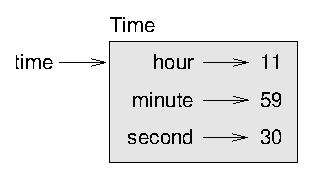
\includegraphics{figs/time.eps}}
\afterfig

\begin{exercise}
\label{printtime}
Write a function called \verb"print_time" that takes a 
Time object and prints it in the form {\tt hour:minute:second}.\\

{\bf Hint:} the format sequence \verb"'%.2d'" prints an integer using
at least two digits, including a leading zero if necessary.
\end{exercise}

\begin{exercise}
\label{is_after}

\index{boolean function}

Write a boolean function called \verb"is_after" that
takes two Time objects, {\tt t1} and {\tt t2}, and
returns {\tt True} if {\tt t1} follows {\tt t2} chronologically and
{\tt False} otherwise. \\

{\bf Challenge:} don't use an {\tt if} statement.
\end{exercise}


\section{Pure functions}

\index{prototype and patch}
\index{development plan!prototype and patch}

In the next few sections, we'll write two functions that add time
values.  They demonstrate two kinds of functions: pure functions and
modifiers.  They also demonstrate a development plan I'll call {\bf
  prototype and patch}, which is a way of tackling a complex problem
by starting with a simple prototype and incrementally dealing with the
complications.

Here is a simple prototype of \verb"add_time":

\beforeverb
\begin{pycode}
def add_time(t1, t2):
    sum = Time()
    sum.hour = t1.hour + t2.hour
    sum.minute = t1.minute + t2.minute
    sum.second = t1.second + t2.second
    return sum
\end{pycode}
\afterverb
%
The function creates a new {\tt Time} object, initializes its
attributes, and returns a reference to the new object.  This is called
a {\bf pure function} because it does not modify any of the objects
passed to it as arguments and it has no effect,
like displaying a value or getting user input, 
other than returning a value.

\index{pure function}
\index{function type!pure}

To test this function, I'll create two Time objects: {\tt start}
contains the start time of a movie, like {\em Monty Python and the
Holy Grail}, and {\tt duration} contains the run time of the movie,
which is one hour 35 minutes.
%
\index{Monty Python and the Holy Grail}
%
\verb"add_time" figures out when the movie will be done.

\beforeverb
\begin{pyinterpreter}
>>> start = Time()
>>> start.hour = 9
>>> start.minute = 45
>>> start.second =  0
>>>
>>> duration = Time()
>>> duration.hour = 1
>>> duration.minute = 35
>>> duration.second = 0
>>>
>>> done = add_time(start, duration)
>>> print_time(done)
10:80:00
\end{pyinterpreter}
\afterverb
%
The result, {\tt 10:80:00} might not be what you were hoping
for.  The problem is that this function does not deal with cases where the
number of seconds or minutes adds up to more than sixty.  When that
happens, we have to ``carry'' the extra seconds into the minute column
or the extra minutes into the hour column.

\index{carrying, addition with}

Here's an improved version:

\beforeverb
\begin{pycode}
def add_time(t1, t2):
    sum = Time()
    sum.hour = t1.hour + t2.hour
    sum.minute = t1.minute + t2.minute
    sum.second = t1.second + t2.second

    if sum.second >= 60:
        sum.second -= 60
        sum.minute += 1

    if sum.minute >= 60:
        sum.minute -= 60
        sum.hour += 1

    return sum
\end{pycode}
\afterverb
%
Although this function is correct, it is starting to get big.
We will see a shorter alternative later.


\section{Modifiers}
\label{increment}

\index{modifier}
\index{function type!modifier}

Sometimes it is useful for a function to modify the objects it gets as
parameters.  In that case, the changes are visible to the caller.
Functions that work this way are called {\bf modifiers}.
%
\index{increment}
%
{\tt increment}, which adds a given number of seconds to a {\tt Time}
object, can be written naturally as a
modifier.  Here is a rough draft:

\beforeverb
\begin{pycode}
def increment(time, seconds):
    time.second += seconds

    if time.second >= 60:
        time.second -= 60
        time.minute += 1

    if time.minute >= 60:
        time.minute -= 60
        time.hour += 1
\end{pycode}
\afterverb
%
The first line performs the basic operation; the remainder deals
with the special cases we saw before.
%
\index{special case}
%
Is this function correct?  What happens if the parameter {\tt seconds}
is much greater than sixty?  
%
In that case, it is not enough to carry
once; we have to keep doing it until {\tt time.second} is less than sixty.
One solution is to replace the {\tt if} statements with {\tt while}
statements.  That would make the function correct, but not
very efficient.

\begin{exercise}
Write a correct version of {\tt increment} that
doesn't contain any loops.
\end{exercise}

Anything that can be done with modifiers can also be done with pure
functions.  In fact, some programming languages only allow pure
functions.  There is some evidence that programs that use pure
functions are faster to develop and less error-prone than programs
that use modifiers.  But modifiers are convenient at times,
and functional programs tend to be less efficient.

In general, I recommend that you write pure functions whenever it is
reasonable and resort to modifiers only if there is a compelling
advantage. 


\begin{exercise}
Write a ``pure'' version of {\tt increment} that creates and returns
a new Time object rather than modifying the parameter.
\end{exercise}


\section{Prototyping versus planning}
\label{prototype}

\index{prototype and patch}
\index{development plan!prototype and patch}
\index{planned development}
\index{development plan!planned}

The development plan I am demonstrating is called ``prototype and
patch.''  For each function, I wrote a prototype that performed the
basic calculation and then tested it, patching errors along the
way.
%
This approach can be effective, especially if you don't yet have a
deep understanding of the problem.  But incremental corrections can
generate code that is unnecessarily complicated---since it deals with
many special cases---and unreliable---since it is hard to know if you
have found all the errors.

An alternative is {\bf planned development}, in which high-level
insight into the problem can make the programming much easier.  In
this case, the insight is that a Time object is really a three-digit
number in base 60 (see \url{wikipedia.org/wiki/Sexagesimal}.)!  The
{\tt second} attribute is the ``ones column,'' the {\tt minute}
attribute is the ``sixties column,'' and the {\tt hour} attribute is
the ``thirty-six hundreds column.''

\index{sexagesimal}

When we wrote \verb"add_time" and {\tt increment}, we were effectively
doing addition in base 60, which is why we had to carry from one
column to the next.
%
\index{carrying, addition with}
%
This observation suggests another approach to the whole problem---we
can convert Time objects to integers and take advantage of the fact
that the computer knows how to do integer arithmetic.  

Here is a function that converts Times to integers:

\beforeverb
\begin{pycode}
def time_to_int(time):
    minutes = time.hour * 60 + time.minute
    seconds = minutes * 60 + time.second
    return seconds
\end{pycode}
\afterverb
%
And here is the function that converts integers to Times
(recall that {\tt divmod} divides the first argument by the second
and returns the quotient and remainder as a tuple).

\index{divmod}

\beforeverb
\begin{pycode}
def int_to_time(seconds):
    time = Time()
    minutes, time.second = divmod(seconds, 60)
    time.hour, time.minute = divmod(minutes, 60)
    return time
\end{pycode}
\afterverb
%
You might have to think a bit, and run some tests, to convince
yourself that these functions are correct.  One way to test them is to
check that \verb"time_to_int(int_to_time(x)) == x" for many values of
{\tt x}.  This is an example of a consistency check.
%
\index{consistency check}
%
Once you are convinced they are correct, you can use them to 
rewrite \verb"add_time":

\beforeverb
\begin{pycode}
def add_time(t1, t2):
    seconds = time_to_int(t1) + time_to_int(t2)
    return int_to_time(seconds)
\end{pycode}
\afterverb
%
This version is shorter than the original, and easier to verify.

\begin{exercise}
Rewrite {\tt increment} using \verb"time_to_int" and \verb"int_to_time".
\end{exercise}

In some ways, converting from base 60 to base 10 and back is harder
than just dealing with times.  Base conversion is more abstract; our
intuition for dealing with time values is better.
%
But if we have the insight to treat times as base 60 numbers and make
the investment of writing the conversion functions (\verb"time_to_int"
and \verb"int_to_time"), we get a program that is shorter, easier to
read and debug, and more reliable.
%
It is also easier to add features later.  For example, imagine
subtracting two Times to find the duration between them.  The
na\"{\i}ve approach would be to implement subtraction with borrowing.
Using the conversion functions would be easier and more likely to be
correct.

\index{subtraction with borrowing}
\index{borrowing, subtraction with}
\index{generalization}

Ironically, sometimes making a problem harder (or more general) makes it
easier (because there are fewer special cases and fewer opportunities
for error).

\begin{exercise}
Implement a function {\tt time\_difference(time1, time2)} which returns the time 
difference between {\tt time1} and {\tt time2}. The returned time must be positive
regardless of {\tt time1} being later or not than {\tt time2}.
\end{exercise}

\section{Debugging}
\index{debugging}

A Time object is well-formed if the values of {\tt minutes} and {\tt
seconds} are between 0 and 60 (including 0 but not 60) and if 
{\tt hours} is positive.  {\tt hours} and {\tt minutes} should be
integral values, but we might allow {\tt seconds} to have a
fraction part.

\index{invariant}

Requirements like these are called {\bf invariants} because
they should always be true.  To put it a different way, if they
are not true, then something has gone wrong.

Writing code to check your invariants can help you detect errors
and find their causes.  For example, you might have a function
like \verb"valid_time" that takes a Time object and returns
{\tt False} if it violates an invariant:

\beforeverb
\begin{pycode}
def valid_time(time):
    if time.hours < 0 or time.minutes < 0 or time.seconds < 0:
        return False
    if time.minutes >= 60 or time.seconds >= 60:
        return False
    return True
\end{pycode}
\afterverb
%
Then at the beginning of each function you could check the
arguments to make sure they are valid:

\index{raise statement}
\index{statement!raise}

\beforeverb
\begin{pycode}
def add_time(t1, t2):
    if not valid_time(t1) or not valid_time(t2):
        raise ValueError('invalid Time object in add_time')
    seconds = time_to_int(t1) + time_to_int(t2)
    return int_to_time(seconds)
\end{pycode}
\afterverb
%
Or you could use an {\tt assert} statement, which checks a given invariant
and raises an exception if it fails:

\index{assert statement}
\index{statement!assert}

\beforeverb
\begin{pycode}
def add_time(t1, t2):
    assert valid_time(t1) and valid_time(t2)
    seconds = time_to_int(t1) + time_to_int(t2)
    return int_to_time(seconds)
\end{pycode}
\afterverb
%
{\tt assert} statements are useful because they distinguish
code that deals with normal conditions from code
that checks for errors.


\section{Glossary}
	
\begin{vocabulary}[prototype and patch:] A development plan that involves
writing a rough draft of a program, testing, and correcting errors as
they are found.
\index{prototype and patch}
\end{vocabulary}
	
\begin{vocabulary}[planned development:] A development plan that involves
high-level insight into the problem and more planning than incremental
development or prototype development.
\index{planned development}
\end{vocabulary}
	
\begin{vocabulary}[pure function:] A function that does not modify any of the objects it
receives as arguments.  Most pure functions are fruitful.
\index{pure function}
\end{vocabulary}
	
\begin{vocabulary}[modifier:] A function that changes one or more of the objects it
receives as arguments.  Most modifiers are fruitless.
\index{modifier}
\end{vocabulary}
	
\begin{vocabulary}[functional programming style:] A style of program design in which the
majority of functions are pure.
\index{functional programming style}
\end{vocabulary}
	
\begin{vocabulary}[invariant:] A condition that should always be true during the
execution of a program.
\index{invariant}
\end{vocabulary}


\section{Exercises}

\begin{exercise}
Write a function called \verb"mul_time" that takes a Time object
and a number and returns a new Time object that contains
the product of the original Time and the number.

Then use \verb"mul_time" to write a function that takes a Time
object that represents the finishing time in a race, and a number
that represents the distance, and returns a Time object that represents
the average pace (time per mile).

\index{running pace}

\end{exercise}

\begin{exercise}

\index{Date class}
\index{class!Date}

Write a class definition for a Date object that has attributes {\tt
  day}, {\tt month} and {\tt year}.  Write a function called
\verb"increment_date" that takes a Date object, {\tt date} and an
integer, {\tt n}, and returns a new Date object that
represents the day {\tt n} days after {\tt date}.  Hint:
``Thirty days hath September...''  Challenge: does your function
deal with leap years correctly?  See \url{wikipedia.org/wiki/Leap_year}.

\end{exercise}


\begin{exercise}

\index{datetime module}
\index{module!datetime}

The {\tt datetime} module provides {\tt date} and {\tt time} objects
that are similar to the Date and Time objects in this chapter, but
they provide a rich set of methods and operators.  Read the
documentation at \url{docs.python.org/lib/datetime-date.html}.

\begin{enumerate}

\item Use the {\tt datetime} module to write a program that
gets the current date and prints the day of the week.

\index{birthday}

\item Write a program that takes a birthday as input
and prints the user's age and the number of days, hours,
minutes and seconds until their next birthday.
\end{enumerate}

\end{exercise}







\chapterimage{chapter_head_1.pdf} % Chapter heading image
\chapter{Classes and methods}


\section{Object-oriented features}

\index{object-oriented programming}

Python is an {\bf object-oriented programming language}, which means
that it provides features that support object-oriented
programming.
%
It is not easy to define object-oriented programming, but we have
already seen some of its characteristics:

\begin{itemize}

\item Programs are made up of object definitions and function
definitions, and most of the computation is expressed in terms
of operations on objects.

\item Each object definition corresponds to some object or concept
in the real world, and the functions that operate on that object
correspond to the ways real-world objects interact.

\end{itemize}

For example, the {\tt Time} class defined in Chapter~\ref{time}
corresponds to the way people record the time of day, and the
functions we defined correspond to the kinds of things people do with
times.  Similarly, the {\tt Point} and {\tt Rectangle} classes
correspond to the mathematical concepts of a point and a rectangle.

So far, we have not taken advantage of the features Python provides to
support object-oriented programming.  These
features are not strictly necessary; most of them provide
alternative syntax for things we have already done.  But in many cases,
the alternative is more concise and more accurately conveys the
structure of the program.

For example, in the {\tt Time} program, there is no obvious
connection between the class definition and the function definitions
that follow.  With some examination, it is apparent that every function
takes at least one {\tt Time} object as an argument.
%
\index{method}
\index{function}
%
This observation is the motivation for {\bf methods}; a method is
a function that is associated with a particular class.
We have seen methods for strings, lists, dictionaries and tuples.
In this chapter, we will define methods for user-defined types.

\index{syntax}
\index{semantics}

Methods are semantically the same as functions, but there are
two syntactic differences:

\begin{itemize}

\item Methods are defined inside a class definition in order
to make the relationship between the class and the method explicit.

\item The syntax for invoking a method is different from the
syntax for calling a function.

\end{itemize}

In the next few sections, we will take the functions from the previous
two chapters and transform them into methods.  This transformation is
purely mechanical; you can do it simply by following a sequence of
steps.  If you are comfortable converting from one form to another,
you will be able to choose the best form for whatever you are doing.


\section{Printing objects}
\label{print_time}

\index{object!printing}

In Chapter~\ref{time}, we defined a class named
{\tt Time} and in Exercise~\ref{printtime}, you 
wrote a function named \verb"print_time":

\beforeverb
\begin{pycode}
class Time(object):
    """represents the time of day.
       attributes: hour, minute, second"""

def print_time(time):
    print('%.2d:%.2d:%.2d' %
          (time.hour, time.minute, time.second))
\end{pycode}
\afterverb
%
To call this function, you have to pass a {\tt Time} object as an
argument:

\beforeverb
\begin{pyinterpreter}
>>> start = Time()
>>> start.hour = 9
>>> start.minute = 45
>>> start.second = 00
>>> print_time(start)
09:45:00
\end{pyinterpreter}
\afterverb
%
To make \verb"print_time" a method, all we have to do is
move the function definition inside the class definition.  Notice
the change in indentation.

\index{indentation}

\beforeverb
\begin{pycode}
class Time(object):
    """represents the time of day.
       attributes: hour, minute, second"""

    def print_time(time):
        print('%.2d:%.2d:%.2d' %
              (time.hour, time.minute, time.second))
\end{pycode}
\afterverb
%


The second (and more concise) way is to use method syntax:

\index{method syntax}

\beforeverb
\begin{pyinterpreter}
>>> start.print_time()
09:45:00
\end{pyinterpreter}
\afterverb
%
In this use of dot notation, \verb"print_time" is the name of the
method (again), and {\tt start} is the object the method is
invoked on, which is called the {\bf subject}.  Just as the
subject of a sentence is what the sentence is about, the subject
of a method invocation is what the method is about.

\index{subject}

Inside the method, the subject is assigned to the first
parameter, so in this case {\tt start} is assigned
to {\tt time}.

\index{self (parameter name)}
\index{parameter!self}

By convention, the first parameter of a method is
called {\tt self}, so it would be more common to write
\verb"print_time" like this:

\beforeverb
\begin{pycode}
class Time(object):
    """represents the time of day.
       attributes: hour, minute, second"""

    def print_time(self):
        print('%.2d:%.2d:%.2d' %
              (self.hour, self.minute, self.second))
\end{pycode}
\afterverb
%
The reason for this convention is an implicit metaphor:

\index{metaphor, method invocation}

\begin{itemize}

\item The syntax for a function call, \verb"print_time(start)",
  suggests that the function is the active agent.  It says something
  like, ``Hey \verb"print_time"!  Here's an object for you to print.''

\item In object-oriented programming, the objects are the active
  agents.  A method invocation like \verb"start.print_time()" says
  ``Hey {\tt start}!  Please print yourself.''

\end{itemize}

This change in perspective might be more polite, but it is not obvious
that it is useful.  In the examples we have seen so far, it may not
be.  But sometimes shifting responsibility from the functions onto the
objects makes it possible to write more versatile functions, and makes
it easier to maintain and reuse code.

\begin{remark}
There is another, less common way to call \verb"print_time" using function syntax:

\index{function syntax}
\index{dot notation}


\beforeverb
\begin{pyinterpreter}
>>> Time.print_time(start)
09:45:00
\end{pyinterpreter}
\afterverb
%
In this use of dot notation, {\tt Time} is the name of the class,
and \verb"print_time" is the name of the method.  {\tt start} is
passed as a parameter.
\end{remark}

\begin{exercise}
\label{convert}
Rewrite \verb"time_to_int"
(from Section~\ref{prototype}) as a method.  It is probably not
appropriate to rewrite \verb"int_to_time" as a method; it's not
clear what object you would invoke it on!
\end{exercise}


\section{Another example}

\index{increment}

Here's a version of {\tt increment} (from Section~\ref{increment})
rewritten as a method:

\beforeverb
\begin{pycode}
# inside class Time:

    def increment(self, seconds):
        seconds += self.time_to_int()
        return int_to_time(seconds)
\end{pycode}
\afterverb
%
This version assumes that \verb"time_to_int" is written
as a method, as in Exercise~\ref{convert}.  Also, note that
it is a pure function, not a modifier.

Here's how you would invoke {\tt increment}:

\beforeverb
\begin{pyinterpreter}
>>> start.print_time()
09:45:00
>>> end = start.increment(1337)
>>> end.print_time()
10:07:17
\end{pyinterpreter}
\afterverb
%
The subject, {\tt start}, gets assigned to the first parameter,
{\tt self}.  The argument, {\tt 1337}, gets assigned to the
second parameter, {\tt seconds}.

This mechanism can be confusing, especially if you make an error.
For example, if you invoke {\tt increment} with two arguments, you
get:

\index{exception!TypeError}
\index{TypeError}

\beforeverb
\begin{pyinterpreter}
>>> end = start.increment(1337, 460)
TypeError: increment() takes exactly 2 arguments (3 given)
\end{pyinterpreter}
\afterverb
%
The error message is initially confusing, because there are
only two arguments in parentheses.  But the subject is also
considered an argument, so all together that's three.


\section{A more complicated example}

\verb"is_after" (from Exercise~\ref{is_after}) is slightly more complicated
because it takes two Time objects as parameters.  In this case it is
conventional to name the first parameter {\tt self} and the second
parameter {\tt other}:

\index{other (parameter name)}
\index{parameter!other}

\beforeverb
\begin{pycode}
# inside class Time:

    def is_after(self, other):
        return self.time_to_int() > other.time_to_int()
\end{pycode}
\afterverb
%
To use this method, you have to invoke it on one object and pass
the other as an argument:

\beforeverb
\begin{pyinterpreter}
>>> end.is_after(start)
True
\end{pyinterpreter}
\afterverb
%
One nice thing about this syntax is that it almost reads
like English: ``end is after start?''


\section{The init method}

\index{init method}
\index{method!init}

The init method (short for ``initialization'') is
a special method that gets invoked when an object is instantiated.  
Its full name is \verb"__init__" (two underscore characters,
followed by {\tt init}, and then two more underscores).  An
init method for the {\tt Time} class might look like this:

\beforeverb
\begin{pycode}
# inside class Time:

    def __init__(self, hour=0, minute=0, second=0):
        self.hour = hour
        self.minute = minute
        self.second = second
\end{pycode}
\afterverb
%
It is common for the parameters of \verb"__init__"
to have the same names as the attributes.  The statement

\beforeverb
\begin{pycode}
        self.hour = hour
\end{pycode}
\afterverb
%
stores the value of the parameter {\tt hour} as an attribute
of {\tt self}.

\index{optional parameter}
\index{parameter!optional}
\index{default value}
\index{override}

The parameters are optional, so if you call {\tt Time} with
no arguments, you get the default values.

\beforeverb
\begin{pyinterpreter}
>>> time = Time()
>>> time.print_time()
00:00:00
\end{pyinterpreter}
\afterverb
%
If you provide one argument, it overrides {\tt hour}:

\beforeverb
\begin{pyinterpreter}
>>> time = Time (9)
>>> time.print_time()
09:00:00
\end{pyinterpreter}
\afterverb
%
If you provide two arguments, they override {\tt hour} and
{\tt minute}.

\beforeverb
\begin{pyinterpreter}
>>> time = Time(9, 45)
>>> time.print_time()
09:45:00
\end{pyinterpreter}
\afterverb
%
And if you provide three arguments, they override all three
default values.


\begin{exercise}
\index{Point class}
\index{class!Point}

Write an init method for the {\tt Point} class that takes
{\tt x} and {\tt y} as optional parameters and assigns
them to the corresponding attributes.
\end{exercise}


\section{The {\tt \_\_str\_\_} method}

\index{str method@\_\_str\_\_ method}
\index{method!\_\_str\_\_}

\verb"__str__" is a special method, like \verb"__init__",
that is supposed to return a string representation of an object.

\index{string representation}

For example, here is a {\tt str} method for Time objects:

\beforeverb
\begin{pycode}
# inside class Time:

    def __str__(self):
        return ('%.2d:%.2d:%.2d'
                % (self.hour, self.minute, self.second))
\end{pycode}
\afterverb
%
When you {\tt print} an object, Python invokes the {\tt str} method:

\index{print statement}
\index{statement!print}

\beforeverb
\begin{pyinterpreter}
>>> time = Time(9, 45)
>>> print(time)
09:45:00
\end{pyinterpreter}
\afterverb
%
When I write a new class, I almost always start by writing 
\verb"__init__", which makes it easier to instantiate objects, and 
\verb"__str__", which is useful for debugging.


\begin{exercise}
Write a {\tt str} method for the {\tt Point} class.  Create
a Point object and print it.
\end{exercise}


\section{Operator overloading}
\label{operator overloading}

By defining other special methods, you can specify the behavior
of operators on user-defined types.  For example, if you define
a method named \verb"__add__" for the {\tt Time} class, you can use the
{\tt +} operator on Time objects.

Here is what the definition might look like:

\index{add method}
\index{method!add}

\beforeverb
\begin{pycode}
# inside class Time:

    def __add__(self, other):
        seconds = self.time_to_int() + other.time_to_int()
        return int_to_time(seconds)
\end{pycode}
\afterverb
%
And here is how you could use it:

\beforeverb
\begin{pyinterpreter}
>>> start = Time(9, 45)
>>> duration = Time(1, 35)
>>> print(start + duration)
11:20:00
\end{pyinterpreter}
\afterverb
%
When you apply the {\tt +} operator to Time objects, Python invokes
\verb"__add__".  When you print the result, Python invokes 
\verb"__str__".  So there is quite a lot happening behind the scenes!

\index{operator overloading}

Changing the behavior of an operator so that it works with
user-defined types is called {\bf operator overloading}.  For every
operator in Python there is a corresponding special method, like 
\verb"__add__".  For more details, see
\url{docs.python.org/ref/specialnames.html}.

\begin{exercise}
Write an {\tt add} method for the Point class.  
\end{exercise}


\section{Type-based dispatch}

In the previous section we added two Time objects, but you
also might want to add an integer to a Time object.  The
following is a version of \verb"__add__"
that checks the type of {\tt other} and invokes either
\verb"add_time" or {\tt increment}:

\beforeverb
\begin{pycode}
# inside class Time:

    def __add__(self, other):
        if isinstance(other, Time):
            return self.add_time(other)
        else:
            return self.increment(other)

    def add_time(self, other):
        seconds = self.time_to_int() + other.time_to_int()
        return int_to_time(seconds)

    def increment(self, seconds):
        seconds += self.time_to_int()
        return int_to_time(seconds)
\end{pycode}
\afterverb
%
The built-in function {\tt isinstance} takes a value and a
class object, and returns {\tt True} if the value is an instance
of the class.

\index{isinstance function}
\index{function!isinstance}

If {\tt other} is a Time object, \verb"__add__" invokes
\verb"add_time".  Otherwise it assumes that the parameter
is a number and invokes {\tt increment}.  This operation is
called a {\bf type-based dispatch} because it dispatches the
computation to different methods based on the type of the
arguments.

\index{type-based dispatch}
\index{dispatch, type-based}

Here are examples that use the {\tt +} operator with different
types:

\beforeverb
\begin{pyinterpreter}
>>> start = Time(9, 45)
>>> duration = Time(1, 35)
>>> print(start + duration)
11:20:00
>>> print(start + 1337)
10:07:17
\end{pyinterpreter}
\afterverb
%
Unfortunately, this implementation of addition is not commutative.
If the integer is the first operand, you get

\index{commutativity}

\beforeverb
\begin{pyinterpreter}
>>> print(1337 + start)
TypeError: unsupported operand type(s) for +: 'int' and 'instance'
\end{pyinterpreter}
\afterverb
%
The problem is, instead of asking the Time object to add an integer,
Python is asking an integer to add a Time object, and it doesn't know
how to do that.  But there is a clever solution for this problem: the
special method \verb"__radd__", which stands for ``right-side add.''
This method is invoked when a Time object appears on the right side of
the {\tt +} operator.  Here's the definition:

\index{radd method}
\index{method!radd}

\beforeverb
\begin{pycode}
# inside class Time:

    def __radd__(self, other):
        return self.__add__(other)
\end{pycode}
\afterverb
%
And here's how it's used:

\beforeverb
\begin{pyinterpreter}
>>> print(1337 + start)
10:07:17
\end{pyinterpreter}
\afterverb
%
Unfortunately we are not done yet. For example, adding a Boolean {\tt True} to 
a time has no sense and should raise an exception. However, our current solution 
allows such operation has shown here:

\beforeverb
\begin{pyinterpreter}
>>> print(start + True)
09:45:01
>>> print(start + 1.1)
09:45:01
\end{pyinterpreter}
\afterverb

The following code solves the issue by managing legal and illegal addition operations, ensuring that only additions with another {\tt Time} object or an {\tt int} are allowed.

\beforeverb
\begin{pycode}
# inside class Time:

    def __add__(self, other):
        if isinstance(other, Time):
            return self.add_time(other)
        elif (isinstance(other, int)
                  and not isinstance(other, bool)):
            return self.increment(other)
        else:
            raise TypeError("can't add Time with " +
                            type(other).__qualname__)
\end{pycode}
\afterverb

We have now achieved the desired behaviour, where trying to do an illegal addition raises an exception. 

\beforeverb
\begin{pyinterpreter}
>>> print(start + True)
Traceback (most recent call last):
...
TypeError: can't add Time with bool

>>> print(start + 1.5)
Traceback (most recent call last):
...
TypeError: can't add Time with float

>>> print(start + '11:05:03')
Traceback (most recent call last):
...
TypeError: can't add Time with str
\end{pyinterpreter}
\afterverb

\begin{remark}
You may have noticed the Boolean expression \pyinline{not isinstance(other, bool)} in the {\tt elif} clause. One could wonder why we needed to this additional condition. As we mentioned earlier in section~\ref{sec:logical-operator}, in Python True and 1 can be used interchangeably, the same applies between {\tt False} and 0. Therefore, adding {\tt True} to an {\tt int} is a valid operation. 

So why don't we allow the the addition between {\tt Time} object and Booleans?

We apply this restriction on the addition operator to preserve the semantic coherence of the {\tt Time} type. The moral of the story is ``It's not because we can do something that we should do it!''. When building new types, it is essential to preserve semantic coherence for this type, and refrain from using any shortcut.
\end{remark}

\begin{exercise}
In most cases it does not make sense to add a string to a {\tt Time}. However, the statement \pyinline{print(start + '11:05:03')} tries to add a {\tt Time} object to a well formatted string representing a valid time. At the moment, the statement raises an exception, change the definition of \verb|__add__| in order to accept well formatted string representing a time value.

{\bf Hint:} The following strings are not well formatted time values:
\begin{itemize}
	\item \verb|':10:15'| needs at least one digit for hours. Can have more than two digits for hours, for example both \verb|'102:10:15'| and \verb|'02:10:15'| are valid.
	\item \verb|'01:1:15'| and \verb|'01:10:1'| are invalid. Both minutes and seconds need {\bf exactly} two digits.
	\item \verb|'01:75:60'| is invalid for two reasons, minutes and seconds must be between {\tt 00} and {\tt 59}.
	\item \verb|'01:01:15.5'| only whole seconds are allowed.
\end{itemize}
\end{exercise}


\begin{exercise}
Write an {\tt add} method for Points that works with either a
Point object or a tuple:  
\begin{itemize}

\item If the second operand is a Point, the method should return a new
Point whose $x$ coordinate is the sum of the $x$ coordinates of the
operands, and likewise for the $y$ coordinates.

\item If the second operand is a tuple, the method should add the
first element of the tuple to the $x$ coordinate and the second
element to the $y$ coordinate, and return a new Point with the result. 

\end{itemize}

\end{exercise}


\section{Polymorphism}

Type-based dispatch is useful when it is necessary, but (fortunately)
it is not always necessary.  Often you can avoid it by writing functions
that work correctly for arguments with different types.

\index{type-based dispatch}
\index{dispatch!type-based}

Many of the functions we wrote for strings will actually
work for any kind of sequence.
For example, in Section~\ref{histogram}
we used {\tt histogram} to count the number of times each letter
appears in a word.

\beforeverb
\begin{pycode}
def histogram(s):
    d = dict()
    for c in s:
        if c not in d:
            d[c] = 1
        else:
            d[c] = d[c]+1
    return d
\end{pycode}
\afterverb
%
This function also works for lists, tuples, and even dictionaries,
as long as the elements of {\tt s} are hashable, so they can be used
as keys in {\tt d}.

\beforeverb
\begin{pyinterpreter}
>>> t = ['spam', 'egg', 'spam', 'spam', 'bacon', 'spam']
>>> histogram(t)
{'bacon': 1, 'egg': 1, 'spam': 4}
\end{pyinterpreter}
\afterverb
%
Functions that can work with several types are called {\bf polymorphic}.
Polymorphism can facilitate code reuse.  For example, the built-in
function {\tt sum}, which adds the elements of a sequence, works
as long as the elements of the sequence support addition.

\index{polymorphism}

Since Time objects provide an {\tt add} method, they work
with {\tt sum}:

\beforeverb
\begin{pyinterpreter}
>>> t1 = Time(7, 43)
>>> t2 = Time(7, 41)
>>> t3 = Time(7, 37)
>>> total = sum([t1, t2, t3])
>>> print(total)
23:01:00
\end{pyinterpreter}
\afterverb
%
In general, if all of the operations inside a function 
work with a given type, then the function works with that type.

The best kind of polymorphism is the unintentional kind, where
you discover that a function you already wrote can be
applied to a type you never planned for.


\section{Debugging}
\index{debugging}

It is legal to add attributes to objects at any point in the execution
of a program, but if you are a stickler for type theory, it is a
dubious practice to have objects of the same type with different
attribute sets.  It is usually a good idea to
initialize all of an objects attributes in the init method.

\index{init method}
\index{attribute!initializing}

If you are not sure whether an object has a particular attribute, you
can use the built-in function {\tt hasattr} (see Section~\ref{hasattr}).

\index{hasattr function}
\index{function!hasattr}
\index{dict attribute@\_\_dict\_\_ attribute}
\index{attribute!\_\_dict\_\_}

Another way to access the attributes of an object is through the
special attribute \verb"__dict__", which is a dictionary that maps
attribute names (as strings) and values:

\beforeverb
\begin{pyinterpreter}
>>> p = Point(3, 4)
>>> print p.__dict__
{'y': 4, 'x': 3}
\end{pyinterpreter}
\afterverb
%
For purposes of debugging, you might find it useful to keep this
function handy:

\beforeverb
\begin{pycode}
def print_attributes(obj):
    for attr in obj.__dict__:
        print attr, getattr(obj, attr)
\end{pycode}
\afterverb
%
\verb"print_attributes" traverses the items in the object's dictionary
and prints each attribute name and its corresponding value.

\index{traversal!dictionary}
\index{dictionary!traversal}

The built-in function {\tt getattr} takes an object and an attribute
name (as a string) and returns the attribute's value.

\index{getattr function}
\index{function!getattr}


\section{Glossary}

\begin{description}

\item[object-oriented language:] A language that provides features,
  such as user-defined classes and method syntax, that facilitate
  object-oriented programming.
\index{object-oriented language}

\item[object-oriented programming:] A style of programming in which
data and the operations that manipulate it are organized into classes
and methods.
\index{object-oriented programming}

\item[method:] A function that is defined inside a class definition and
is invoked on instances of that class.
\index{method}

\item[subject:] The object a method is invoked on.
\index{subject}

\item[operator overloading:] Changing the behavior of an operator like
{\tt +} so it works with a user-defined type.
\index{overloading}
\index{operator!overloading}

\item[type-based dispatch:] A programming pattern that checks the type
of an operand and invokes different functions for different types.
\index{type-based dispatch}

\item[polymorphic:] Pertaining to a function that can work with more
  than one type.  

\index{polymorphism}

\end{description}

\section{Exercises}

\begin{exercise}

\index{default value!avoiding mutable}
\index{mutable object, as default value}
\index{worst bug}
\index{bug!worst}

This exercise is a cautionary tale about one of the most
common, and difficult to find, errors in Python.

\begin{enumerate}

\index{Kangaroo class}
\index{class!Kangaroo}

\item Write a definition for a class named {\tt Kangaroo} with the following
methods:

\begin{enumerate}

\item An \verb"__init__" method that initializes an attribute named 
\verb"pouch_contents" to an empty list.

\item A method named \verb"put_in_pouch" that takes an object
of any type and adds it to \verb"pouch_contents".

\item A \verb"__str__" method that returns a string representation
of the Kangaroo object and the contents of the pouch.

\end{enumerate}
%
Test your code 
by creating two {\tt Kangaroo} objects, assigning them to variables
named {\tt kanga} and {\tt roo}, and then adding {\tt roo} to the
contents of {\tt kanga}'s pouch.

\item Download \url{thinkpython.com/code/BadKangaroo.py}.  It contains
a solution to the previous problem with one big, nasty bug.
Find and fix the bug.

If you get stuck, you can download
\url{thinkpython.com/code/GoodKangaroo.py}, which explains the
problem and demonstrates a solution.

\index{aliasing}
\index{embedded object}
\index{object!embedded}

\end{enumerate}


\end{exercise}




%\begin{exercise}
%
%\index{Visual module}
%\index{module!Visual}
%\index{vpython module}
%\index{module!vpython}
%
%Visual is a Python module that provides 3-D graphics.  It is
%not always included in a Python installation, so you might have
%to install it from your software repository or, if it's not there,
%from \url{vpython.org}.
%
%The following example creates a 3-D space that is 256 units
%wide, long and high, and sets the ``center'' to be the
%point $(128, 128, 128)$.  Then it draws a blue sphere.
%
%\beforeverb
%\begin{pyexo}
%from visual import *
%
%scene.range = (256, 256, 256)
%scene.center = (128, 128, 128)
%
%color = (0.1, 0.1, 0.9)          # mostly blue
%sphere(pos=scene.center, radius=128, color=color)
%\end{pyexo}
%\afterverb
%
%{\tt color} is an RGB tuple; that is, the elements are Red-Green-Blue
%levels between 0.0 and 1.0 (see
%\url{wikipedia.org/wiki/RGB_color_model}).
%
%If you run this code, you should see a window with a black
%background and a blue sphere.  If you drag the middle button
%up and down, you can zoom in and out.  You can also rotate
%the scene by dragging the right button, but with only one
%sphere in the world, it is hard to tell the difference.
%
%The following loop creates a cube of spheres:
%
%\beforeverb
%\begin{pyexo}
%t = range(0, 256, 51)
%for x in t:
    %for y in t:
        %for z in t:
            %pos = x, y, z
            %sphere(pos=pos, radius=10, color=color)
%\end{pyexo}
%\end{pyexo}
%\afterverb
%
%\begin{enumerate}
%
%\item Put this code in a script and make sure it works for
%you.
%
%\item Modify the program so that each sphere in the cube
%has the color that corresponds to its position in RGB space.
%Notice that the coordinates are in the range 0--255, but
%the RGB tuples are in the range 0.0--1.0.
%
%\index{color list}
%\index{available colors}
%
%%\item Download \url{thinkpython.com/code/color_list.py}
%%and use the function \verb"read_colors" to generate a list
%%of the available colors on your system, their names and
%%RGB values.  For each named color draw a sphere in the
%%position that corresponds to its RGB values.
%
%
%
%\end{enumerate}
%
%%You can see my solution at \url{thinkpython.com/code/color_space.py}.
%
%\end{exercise}
%

\chapter{Inheritance}

In this chapter we will develop classes to represent playing cards,
decks of cards, and poker hands.  If you don't play poker, you can
read about it at \url{wikipedia.org/wiki/Poker}, but you don't have
to; I'll tell you what you need to know for the exercises.

\index{playing card, Anglo-American}
\index{card, playing}
\index{poker}

If you are not familiar with Anglo-American playing cards,
you can read about them at \url{wikipedia.org/wiki/Playing_cards}.


\section{Card objects}

There are fifty-two cards in a deck, each of which belongs to one of
four suits and one of thirteen ranks.  The suits are Spades, Hearts,
Diamonds, and Clubs (in descending order in bridge).  The ranks are
Ace, 2, 3, 4, 5, 6, 7, 8, 9, 10, Jack, Queen, and King.  Depending on
the game that you are playing, an Ace may be higher than King
or lower than 2.

\index{rank}
\index{suit}

If we want to define a new object to represent a playing card, it is
obvious what the attributes should be: {\tt rank} and
{\tt suit}.  It is not as obvious what type the attributes
should be.  One possibility is to use strings containing words like
\verb"'Spade'" for suits and \verb"'Queen'" for ranks.  One problem with
this implementation is that it would not be easy to compare cards to
see which had a higher rank or suit.

\index{encode}
\index{encrypt}
\index{map to}
\index{representation}

An alternative is to use integers to {\bf encode} the ranks and suits.
In this context, ``encode'' means that we are going to define a mapping
between numbers and suits, or between numbers and ranks.  This
kind of encoding is not meant to be a secret (that
would be ``encryption'').

For example, this table shows the suits and the corresponding integer
codes:

\beforefig
\begin{tabular}{l c l}
Spades & $\mapsto$ & 3 \\
Hearts & $\mapsto$ & 2 \\
Diamonds & $\mapsto$ & 1 \\
Clubs & $\mapsto$ & 0
\end{tabular}
\afterfig

This code makes it easy to compare cards; because higher suits map to
higher numbers, we can compare suits by comparing their codes.

The mapping for ranks is fairly obvious; each of the numerical ranks
maps to the corresponding integer, and for face cards:

\beforefig
\begin{tabular}{l c l}
Jack & $\mapsto$ & 11 \\
Queen & $\mapsto$ & 12 \\
King & $\mapsto$ & 13 \\
\end{tabular}
\afterfig

I am using the $\mapsto$ symbol to make it clear that these mappings
are not part of the Python program.  They are part of the program
design, but they don't appear explicitly in the code.

\index{Card class}
\index{class!Card}

The class definition for {\tt Card} looks like this:

\beforeverb
\begin{pycode}
class Card(object):
    """represents a standard playing card."""

    def __init__(self, suit=0, rank=2):
        self.suit = suit
        self.rank = rank
\end{pycode}
\afterverb
%
As usual, the init method takes an optional
parameter for each attribute.  The default card is
the 2 of Clubs.

\index{init method}
\index{method!init}

To create a Card, you call {\tt Card} with the
suit and rank of the card you want.

\beforeverb
\begin{pycode}
queen_of_diamonds = Card(1, 12)
\end{pycode}
\afterverb
%


\section{Class attributes}

\index{class attribute}
\index{attribute!class}

In order to print Card objects in a way that people can easily
read, we need a mapping from the integer codes to the corresponding
ranks and suits.  A natural way to
do that is with lists of strings.  We assign these lists to {\bf class
attributes}:

\beforeverb
\begin{pycode}
# inside class Card:

    suit_names = ['Clubs', 'Diamonds', 'Hearts', 'Spades']
    rank_names = [None, 'Ace', '2', '3', '4', '5', '6', '7', 
              '8', '9', '10', 'Jack', 'Queen', 'King']

    def __str__(self):
        return '%s of %s' % (Card.rank_names[self.rank],
                             Card.suit_names[self.suit])
\end{pycode}
\afterverb
%
Variables like \verb"suit_names" and \verb"rank_names", which are
defined inside a class but outside of any method, are called
class attributes because they are associated with the class object 
{\tt Card}.

\index{instance attribute}
\index{attribute!instance}

This term distinguishes them from variables like {\tt suit} and {\tt
  rank}, which are called {\bf instance attributes} because they are
associated with a particular instance.

\index{dot notation}

Both kinds of attribute are accessed using dot notation.  For
example, in \verb"__str__", {\tt self} is a Card object,
and {\tt self.rank} is its rank.  Similarly, {\tt Card}
is a class object, and \verb"Card.rank_names" is a
list of strings associated with the class.

Every card has its own {\tt suit} and {\tt rank}, but there
is only one copy of \verb"suit_names" and \verb"rank_names".

Putting it all together, the expression
\verb"Card.rank_names[self.rank]" means ``use the attribute {\tt rank}
from the object {\tt self} as an index into the list \verb"rank_names"
from the class {\tt Card}, and select the appropriate string.''

The first element of \verb"rank_names" is {\tt None} because there
is no card with rank zero.  By including {\tt None} as a place-keeper,
we get a mapping with the nice property that the index 2 maps to the
string \verb"'2'", and so on.  To avoid this tweak, we could have
used a dictionary instead of a list.

With the methods we have so far, we can create and print cards:

\beforeverb
\begin{pyinterpreter}
>>> card1 = Card(2, 11)
>>> print card1
Jack of Hearts
\end{pyinterpreter}
\afterverb
%
Here is a diagram that shows the {\tt Card} class object
and one Card instance:

\index{state diagram}
\index{diagram!state}
\index{object diagram}
\index{diagram!object}

\beforefig
\centerline{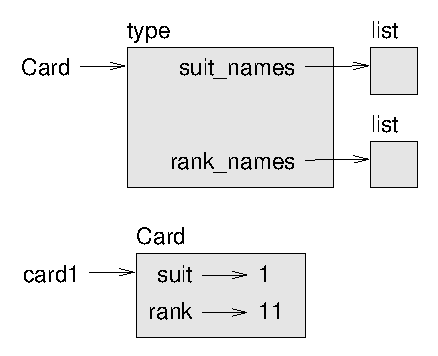
\includegraphics{figs/card1.eps}}
\afterfig

{\tt Card} is a class object, so it has type {\tt type}.  {\tt
card1} has type {\tt Card}.  (To save space, I didn't draw the
contents of \verb"suit_names" and \verb"rank_names").


\section{Comparing cards}
\label{comparecard}

\index{operator!relational}
\index{relational operator}

For built-in types, there are relational operators
({\tt <}, {\tt >}, {\tt ==}, etc.)
that compare
values and determine when one is greater than, less than, or equal to
another.  For user-defined types, we can override the behavior of
the built-in operators by providing a method named
\verb"__cmp__".  

\verb"__cmp__" takes two parameters, {\tt self} and {\tt other},
and returns a positive number if the first object is greater, a
negative number if the second object is greater, and 0 if they are
equal to each other.

\index{override}
\index{operator overloading}

The correct ordering for cards is not obvious.
For example, which
is better, the 3 of Clubs or the 2 of Diamonds?  One has a higher
rank, but the other has a higher suit.  In order to compare
cards, you have to decide whether rank or suit is more important.

The answer might depend on what game you are playing, but to keep
things simple, we'll make the arbitrary choice that suit is more
important, so all of the Spades outrank all of the Diamonds,
and so on.

\index{cmp method@\_\_cmp\_\_ method}
\index{method!\_\_cmp\_\_}

With that decided, we can write \verb"__cmp__":

\beforeverb
\begin{pycode}
# inside class Card:

    def __cmp__(self, other):
        # check the suits
        if self.suit > other.suit: return 1
        if self.suit < other.suit: return -1

        # suits are the same... check ranks
        if self.rank > other.rank: return 1
        if self.rank < other.rank: return -1

        # ranks are the same... it's a tie
        return 0    
\end{pycode}
\afterverb
%
You can write this more concisely using tuple comparison:

\index{tuple!comparison}
\index{comparison!tuple}

\beforeverb
\begin{pycode}
# inside class Card:

    def __cmp__(self, other):
        t1 = self.suit, self.rank
        t2 = other.suit, other.rank
        return cmp(t1, t2)
\end{pycode}
\afterverb
%
The built-in function {\tt cmp} has the same interface as
the method \verb"__cmp__": it takes two values and returns
a positive number if the first is larger, a negative number
if the second is larger, and 0 if they are equal.

\index{cmp function}
\index{function!cmp}


\begin{exercise}
Write a \verb"__cmp__" method for Time objects.  Hint: you
can use tuple comparison, but you also might consider using
integer subtraction.

%    def __cmp__(self, other):
%        return time_to_int(self) - time_to_int(other)

%If {\tt self} is later than {\tt other}, the result is
%a positive number.  If {\tt other} is later, the result
%is negative.  And if {\tt self} and {\tt other} are equal
%(but not necessarily identical)
%the result is zero.

\end{exercise}


\section{Decks}
\index{list!of objects}
\index{deck, playing cards}

Now that we have Cards, the next step is to define Decks.  Since a
deck is made up of cards, it is natural for each Deck to contain a
list of cards as an attribute.

\index{init method}
\index{method!init}

The following is a class definition for {\tt Deck}.  The
init method creates the attribute {\tt cards} and generates
the standard set of fifty-two cards:

\index{composition}
\index{loop!nested}

\index{Deck class}
\index{class!Deck}

\beforeverb
\begin{pycode}
class Deck(object):

    def __init__(self):
        self.cards = []
        for suit in range(4):
            for rank in range(1, 14):
                card = Card(suit, rank)
                self.cards.append(card)
\end{pycode}
\afterverb
%
The easiest way to populate the deck is with a nested loop.  The outer
loop enumerates the suits from 0 to 3.  The inner loop enumerates the
ranks from 1 to 13.  Each iteration
creates a new Card with the current suit and rank,
and appends it to {\tt self.cards}.

\index{append method}
\index{method!append}


\section{Printing the deck}
\label{printdeck}

\index{str method@\_\_str\_\_ method}
\index{method!\_\_str\_\_}

Here is a \verb"__str__" method for {\tt Deck}:

\beforeverb
\begin{pycode}
#inside class Deck:

    def __str__(self):
        res = []
        for card in self.cards:
            res.append(str(card))
        return '\n'.join(res)
\end{pycode}
\afterverb
%
This method demonstrates an efficient way to accumulate a large
string: building a list of strings and then using {\tt join}.
The built-in function {\tt str} invokes the \verb"__str__"
method on each card and returns the string representation.

\index{accumulator!string}
\index{string!accumulator}
\index{join method}
\index{method!join}
\index{newline}

Since we invoke {\tt join} on a newline character, the cards
are separated by newlines.  Here's what the result looks like:

\beforeverb
\begin{pyinterpreter}
>>> deck = Deck()
>>> print deck
Ace of Clubs
2 of Clubs
3 of Clubs
...
10 of Spades
Jack of Spades
Queen of Spades
King of Spades
\end{pyinterpreter}
\afterverb
%
Even though the result appears on 52 lines, it is
one long string that contains newlines.


\section{Add, remove, shuffle and sort}

To deal cards, we would like a method that
removes a card from the deck and returns it.
The list method {\tt pop} provides a convenient way to do that:

\index{pop method}
\index{method!pop}

\beforeverb
\begin{pycode}
#inside class Deck:

    def pop_card(self):
        return self.cards.pop()
\end{pycode}
\afterverb
%
Since {\tt pop} removes the {\em last} card in the list, we are
dealing from the bottom of the deck.  In real life bottom dealing is
frowned upon\footnote{See \url{wikipedia.org/wiki/Bottom_dealing}},
but in this context it's ok.

\index{append method}
\index{method!append}

To add a card, we can use the list method {\tt append}:

\beforeverb
\begin{pycode}
#inside class Deck:

    def add_card(self, card):
        self.cards.append(card)
\end{pycode}
\afterverb
%
A method like this that uses another function without doing
much real work is sometimes called a {\bf veneer}.  The metaphor
comes from woodworking, where it is common to glue a thin
layer of good quality wood to the surface of a cheaper piece of
wood.

\index{veneer}

In this case we are defining a ``thin'' method that expresses
a list operation in terms that are appropriate for decks.

As another example, we can write a Deck method named {\tt shuffle}
using the function {\tt shuffle} from the {\tt random} module:

\index{random module}
\index{module!random}
\index{shuffle function}
\index{function!shuffle}

\beforeverb
\begin{pycode}
# inside class Deck:
            
    def shuffle(self):
        random.shuffle(self.cards)
\end{pycode}
\afterverb
%
Don't forget to import {\tt random}.

\begin{exercise}
\index{sort method}
\index{method!sort}

Write a Deck method named {\tt sort} that uses the list method
{\tt sort} to sort the cards in a {\tt Deck}.  {\tt sort} uses
the \verb"__cmp__" method we defined to determine sort order.
\end{exercise}



\section{Inheritance}

\index{inheritance}
\index{object-oriented programming}

The language feature most often associated with object-oriented
programming is {\bf inheritance}.  Inheritance is the ability to
define a new class that is a modified version of an existing
class.

\index{parent class}
\index{child class}
\index{class!child}
\index{subclass}
\index{superclass}

It is called ``inheritance'' because the new class inherits the
methods of the existing class.  Extending this metaphor, the existing
class is called the {\bf parent} and the new class is
called the {\bf child}.

As an example, let's say we want a class to represent a ``hand,''
that is, the set of cards held by one player.  A hand is similar to a
deck: both are made up of a set of cards, and both require operations
like adding and removing cards.

A hand is also different from a deck; there are operations we want for
hands that don't make sense for a deck.  For example, in poker we
might compare two hands to see which one wins.  In bridge, we might
compute a score for a hand in order to make a bid.

This relationship between classes---similar, but different---lends
itself to inheritance.  

The definition of a child class is like other class definitions,
but the name of the parent class appears in parentheses:

\index{parentheses!parent class in}
\index{parent class}
\index{class!parent}
\index{Hand class}
\index{class!Hand}

\beforeverb
\begin{pycode}
class Hand(Deck):
    """represents a hand of playing cards"""
\end{pycode}
\afterverb
%
This definition indicates that {\tt Hand} inherits from {\tt Deck};
that means we can use methods like \verb"pop_card" and \verb"add_card"
for Hands as well as Decks.

{\tt Hand} also inherits \verb"__init__" from {\tt Deck}, but
it doesn't really do what we want: instead of populating the hand
with 52 new cards, the init method for Hands should initialize
{\tt cards} with an empty list.

\index{override}
\index{init method}
\index{method!init}

If we provide an init method in the {\tt Hand} class, it overrides the
one in the {\tt Deck} class:

\beforeverb
\begin{pycode}
# inside class Hand:

    def __init__(self, label=''):
        self.cards = []
        self.label = label
\end{pycode}
\afterverb
%
So when you create a Hand, Python invokes this init method:

\beforeverb
\begin{pyinterpreter}
>>> hand = Hand('new hand')
>>> print hand.cards
[]
>>> print hand.label
new hand
\end{pyinterpreter}
\afterverb
%
But the other methods are inherited from {\tt Deck}, so we can use
\verb"pop_card" and \verb"add_card" to deal a card:

\beforeverb
\begin{pyinterpreter}
>>> deck = Deck()
>>> card = deck.pop_card()
>>> hand.add_card(card)
>>> print hand
King of Spades
\end{pyinterpreter}
\afterverb
%
A natural next step is to encapsulate this code in a method
called \verb"move_cards":

\index{encapsulation}

\beforeverb
\begin{pycode}
#inside class Deck:

    def move_cards(self, hand, num):
        for i in range(num):
            hand.add_card(self.pop_card())
\end{pycode}
\afterverb
%
\verb"move_cards" takes two arguments, a Hand object and the number of
cards to deal.  It modifies both {\tt self} and {\tt hand}, and
returns {\tt None}.

In some games, cards are moved from one hand to another,
or from a hand back to the deck.  You can use \verb"move_cards"
for any of these operations: {\tt self} can be either a Deck
or a Hand, and {\tt hand}, despite the name, can also be a {\tt Deck}.

\begin{exercise}
Write a Deck method called \verb"deal_hands" that takes two
parameters, the number of hands and the number of cards per
hand, and that creates new Hand objects, deals the appropriate
number of cards per hand, and returns a list of Hand objects.
\end{exercise}

Inheritance is a useful feature.  Some programs that would be
repetitive without inheritance can be written more elegantly
with it.  Inheritance can facilitate code reuse, since you can
customize the behavior of parent classes without having to modify
them.  In some cases, the inheritance structure reflects the natural
structure of the problem, which makes the program easier to
understand.

On the other hand, inheritance can make programs difficult to read.
When a method is invoked, it is sometimes not clear where to find its
definition.  The relevant code may be scattered among several modules.
Also, many of the things that can be done using inheritance can be
done as well or better without it.  


\section{Class diagrams}

So far we have seen stack diagrams, which show the state of
a program, and object diagrams, which show the attributes
of an object and their values.  These diagrams represent a snapshot
in the execution of a program, so they change as the program
runs.

They are also highly detailed; for some purposes, too
detailed.  A class diagram is a more abstract representation
of the structure of a program.  Instead of showing individual
objects, it shows classes and the relationships between them.

There are several kinds of relationship between classes:

\begin{itemize}

\item Objects in one class might contain references to objects
in another class.  For example, each Rectangle contains a reference
to a Point, and each Deck contains references to many Cards.
This kind of relationship is called {\bf HAS-A}, as in, ``a Rectangle
has a Point.''

\item One class might inherit from another.  This relationship
is called {\bf IS-A}, as in, ``a Hand is a kind of a Deck.''

\item One class might depend on another in the sense that changes
in one class would require changes in the other.

\end{itemize}

\index{IS-A relationship}
\index{HAS-A relationship}
\index{class diagram}
\index{diagram!class}
\index{UML}

A {\bf class diagram} is a graphical representation of these
relationships\footnote{The diagrams I am using here are similar to UML
  (see \url{wikipedia.org/wiki/Unified_Modeling_Language}), with a few
  simplifications.}.  For example, this diagram shows the
relationships between {\tt Card}, {\tt Deck} and {\tt Hand}.

\beforefig
\centerline{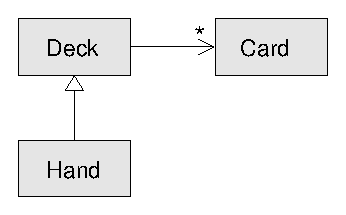
\includegraphics{figs/class1.eps}}
\afterfig

The arrow with a hollow triangle head represents an IS-A
relationship; in this case it indicates that Hand inherits
from Deck.

The standard arrow head represents a HAS-A
relationship; in this case a Deck has references to Card
objects.

\index{multiplicity (in class diagram)}

The star ({\tt *}) near the arrow head is a 
{\bf multiplicity}; it indicates how many Cards a Deck has.
A multiplicity can be a simple number, like {\tt 52}, a range,
like {\tt 5..7} or a star, which indicates that a Deck can
have any number of Cards.

A more detailed diagram might show that a Deck actually
contains a {\em list} of Cards, but built-in types
like list and dict are usually not included in class diagrams.

\begin{exercise}
Read {\tt TurtleWorld.py}, {\tt World.py} and {\tt Gui.py}
and draw a class diagram that shows the relationships among
the classes defined there.
\end{exercise}


\section{Debugging}
\index{debugging}

Inheritance can make debugging a challenge because when you
invoke a method on an object, you might not know which method
will be invoked.

\index{polymorphism}

Suppose you are writing a function that works with Hand objects.
You would like it to work with all kinds of Hands, like
PokerHands, BridgeHands, etc.  If you invoke a method like
{\tt shuffle}, you might get the one defined in {\tt Deck},
but if any of the subclasses override this method, you'll
get that version instead.  

\index{flow of execution}

Any time you are unsure about the flow of execution through your
program, the simplest solution is to add print statements at the
beginning of the relevant methods.  If {\tt Deck.shuffle} prints a
message that says something like {\tt Running Deck.shuffle}, then as
the program runs it traces the flow of execution.

As an alternative, you could use this function, which takes an
object and a method name (as a string) and returns the class that
provides the definition of the method:

\beforeverb
\begin{pycode}
def find_defining_class(obj, meth_name):
    for ty in type(obj).mro():
        if meth_name in ty.__dict__:
            return ty
\end{pycode}
\afterverb
%
Here's an example:

\beforeverb
\begin{pyinterpreter}
>>> hand = Hand()
>>> print find_defining_class(hand, 'shuffle')
<class 'Card.Deck'>
\end{pyinterpreter}
\afterverb
%
So the {\tt shuffle} method for this Hand is the one in {\tt Deck}.

\index{mro method}
\index{method!mro}
\index{method resolution order}

\verb"find_defining_class" uses the {\tt mro} method to get the list
of class objects (types) that will be searched for methods.  ``MRO''
stands for ``method resolution order.''

\index{override}
\index{interface}
\index{precondition}
\index{postcondition}

Here's a program design suggestion: whenever you override a method,
the interface of the new method should be the same as the old.  It
should take the same parameters, return the same type, and obey the
same preconditions and postconditions.  If you obey this rule, you
will find that any function designed to work with an instance of a
superclass, like a Deck, will also work with instances of subclasses
like a Hand or PokerHand.

If you violate this rule, your code will collapse like (sorry)
a house of cards.


\section{Glossary}

\begin{description}

\item[encode:]  To represent one set of values using another
set of values by constructing a mapping between them.
\index{encode}

\item[class attribute:] An attribute associated with a class
object.  Class attributes are defined inside
a class definition but outside any method.
\index{class attribute}
\index{attribute!class}

\item[instance attribute:] An attribute associated with an
instance of a class.
\index{instance attribute}
\index{attribute!instance}

\item[veneer:] A method or function that provides a different
interface to another function without doing much computation.
\index{veneer}

\item[inheritance:] The ability to define a new class that is a
modified version of a previously defined class.
\index{inheritance}

\item[parent class:] The class from which a child class inherits.
\index{parent class}

\item[child class:] A new class created by inheriting from an
existing class; also called a ``subclass.''
\index{child class}
\index{class!child}

\item[IS-A relationship:] The relationship between a child class
and its parent class.
\index{IS-A relationship}

\item[HAS-A relationship:] The relationship between two classes
where instances of one class contain references to instances of
the other.
\index{HAS-A relationship}

\item[class diagram:] A diagram that shows the classes in a program
and the relationships between them.
\index{class diagram}
\index{diagram!class}

\item[multiplicity:] A notation in a class diagram that shows, for
a HAS-A relationship, how many references there are to instances
of another class.
\index{multiplicity (in class diagram)}

\end{description}


\section{Exercises}

\begin{exercise}
\index{poker}


The following are the possible hands in poker, in increasing order
of value (and decreasing order of probability):

\begin{description}

\item[pair:] two cards with the same rank
\vspace{-0.05in}

\item[two pair:] two pairs of cards with the same rank
\vspace{-0.05in}

\item[three of a kind:] three cards with the same rank
\vspace{-0.05in}

\item[straight:] five cards with ranks in sequence (aces can
be high or low, so {\tt Ace-2-3-4-5} is a straight and so is {\tt
10-Jack-Queen-King-Ace}, but {\tt Queen-King-Ace-2-3} is not.)
\vspace{-0.05in}

\item[flush:] five cards with the same suit
\vspace{-0.05in}

\item[full house:] three cards with one rank, two cards with another
\vspace{-0.05in}

\item[four of a kind:] four cards with the same rank
\vspace{-0.05in}

\item[straight flush:] five cards in sequence (as defined above) and
with the same suit
\vspace{-0.05in}

\end{description}
%
The goal of these exercises is to estimate
the probability of drawing these various hands.

\begin{enumerate}

\item Download the following files from \url{thinkpython.com/code}:

\begin{description}

\item[{\tt Card.py}]: A complete version of the {\tt Card},
{\tt Deck} and {\tt Hand} classes in this chapter.

\item[{\tt PokerHand.py}]: An incomplete implementation of a class
that represents a poker hand, and some code that tests it.

\end{description}
%
\item If you run {\tt PokerHand.py}, it deals seven 7-card poker hands
and checks to see if any of them contains a flush.  Read this
code carefully before you go on.

\item Add methods to {\tt PokerHand.py} named \verb"has_pair",
\verb"has_twopair", etc. that return True or False according to
whether or not the hand meets the relevant criteria.  Your code should
work correctly for ``hands'' that contain any number of cards
(although 5 and 7 are the most common sizes).

\item Write a method named {\tt classify} that figures out
the highest-value classification for a hand and sets the
{\tt label} attribute accordingly.  For example, a 7-card hand
might contain a flush and a pair; it should be labeled ``flush''.

\item When you are convinced that your classification methods are
working, the next step is to estimate the probabilities of the various
hands.  Write a function in {\tt PokerHand.py} that shuffles a deck of
cards, divides it into hands, classifies the hands, and counts the
number of times various classifications appear.

\item Print a table of the classifications and their probabilities.
Run your program with larger and larger numbers of hands until the
output values converge to a reasonable degree of accuracy.  Compare
your results to the values at \url{wikipedia.org/wiki/Hand_rankings}.

\end{enumerate}
\end{exercise}


\begin{exercise}

\index{Swampy}
\index{TurtleWorld}

This exercise uses TurtleWorld from Chapter~\ref{turtlechap}.
You will write code that makes Turtles play tag.  If you
are not familiar with the rules of tag, see
\url{wikipedia.org/wiki/Tag_(game)}.

\begin{enumerate}

\item Download \url{thinkpython.com/code/Wobbler.py} and run it.  You
should see a TurtleWorld with three Turtles.  If you press the
{\sf Run} button, the Turtles wander at random.

\item Read the code and make sure you understand how it works.
The {\tt Wobbler} class inherits from {\tt Turtle}, which means
that the {\tt Turtle} methods {\tt lt}, {\tt rt}, {\tt fd}
and {\tt bk} work on Wobblers.

The {\tt step} method gets invoked by TurtleWorld.  It invokes 
{\tt steer}, which turns the Turtle in the desired direction,
{\tt wobble}, which makes a random turn in proportion to the Turtle's
clumsiness, and {\tt move}, which moves forward a few pixels,
depending on the Turtle's speed.

\index{Tagger}

\item Create a file named {\tt Tagger.py}.  Import everything from
  {\tt Wobbler}, then define a class named {\tt Tagger} that inherits
  from {\tt Wobbler}.  Call \verb"make_world" passing the {\tt
    Tagger} class object as an argument.

\item Add a {\tt steer} method to {\tt Tagger} to override the one in
  {\tt Wobbler}.  As a starting place, write a version that always
  points the Turtle toward the origin.  Hint: use the math function
  {\tt atan2} and the Turtle attributes {\tt x}, {\tt y} and
  {\tt heading}.

\item Modify {\tt steer} so that the Turtles stay in bounds.
  For debugging, you might want to use the {\sf Step} button,
  which invokes {\tt step} once on each Turtle.

\item Modify {\tt steer} so that each Turtle points toward its nearest
  neighbor.  Hint: Turtles have an attribute, {\tt world}, that is a
  reference to the TurtleWorld they live in, and the TurtleWorld has
  an attribute, {\tt animals}, that is a list of all Turtles in the
  world.

\item Modify {\tt steer} so the Turtles play tag.  You can add methods
  to {\tt Tagger} and you can override {\tt steer} and
  \verb"__init__", but you may not modify or override {\tt step}, {\tt
    wobble} or {\tt move}.  Also, {\tt steer} is allowed to change the
  heading of the Turtle but not the position.

Adjust the rules and your {\tt steer} method for good quality play;
for example, it should be possible for the slow Turtle to tag the
faster Turtles eventually.

\end{enumerate}

You can get my solution from \url{thinkpython.com/code/Tagger.py}.
\end{exercise}




%----------------------------------------------------------------------------------------
%	BIBLIOGRAPHY
%----------------------------------------------------------------------------------------

%\chapter*{Bibliography}
%\addcontentsline{toc}{chapter}{\textcolor{ocre}{Bibliography}}

%------------------------------------------------

%\section*{Articles}
%\addcontentsline{toc}{section}{Articles}
%\printbibliography[heading=bibempty,type=article]

%------------------------------------------------

%\section*{Books}
%\addcontentsline{toc}{section}{Books}
%\printbibliography[heading=bibempty,type=book]

%----------------------------------------------------------------------------------------
%	INDEX
%----------------------------------------------------------------------------------------

%\cleardoublepage
%\phantomsection
%\setlength{\columnsep}{0.75cm}
%\addcontentsline{toc}{chapter}{\textcolor{ocre}{Index}}
%\printindex

%----------------------------------------------------------------------------------------


\end{document}
